\appendix
\addcontentsline{toc}{chapter}{Appendices}
\startcontents
\startlist[appendix]{lof}
\startlist[appendix]{lot}
\printcontents{atoc}{0}{\chapter*{Appendices}}
\begingroup
\let\clearpage\relax
\singlespacing
\printlist[appendix]{lot}{}{\chapter*{List of Tables}}
\printlist[appendix]{lof}{}{\chapter*{List of Figures}}
\endgroup

\chapter{Tables}
\label{app:Tables}

%\section{Additional tables}

\section{Chapter 3 Tables}

\begin{table}[htbp]
\renewcommand{\arraystretch}{0.7}
%\setlength{\tabcolsep}{20pt} only to stretch the columns if you want
\centering
\begin{tabular}{@{} c c c c c}
\toprule
                   &                    &               & \textbf{TSS enrichment} &     \\
\textbf{Cell type} & \textbf{Condition} & \textbf{CTL1} & \textbf{CTL2} & \textbf{CTL3} \\
\midrule
\midrule
      & Fresh	 & 17.4 & 19.6 & 14.11\\
CD14	& Frozen & 26.3 & 25.2 & 27.1 \\
      & Fixed	 & 2.5  & 16.5 & 22.4 \\
\midrule
      & Fresh	 & 5.3  & 5.6  & 7.7 \\
CD4	  & Frozen & 17.9 & 14.1 & 16.1 \\
      & Fixed	 & 7.9  & 23.0 & 14.3 \\
\bottomrule
\end{tabular}
\medskip %gap
\caption[Enrichment of ATAC-seq reads across the TSS for the CD14$^+$ monocytes and CD4$^+$ samples fresh, frozen and fixed.]{\textbf{Enrichment of ATAC-seq reads across the TSS for the CD14$^+$ monocytes and CD4$^+$ samples fresh, frozen and fixed.}}
\label{tab:Core_ATAC_TSS_summary_table}
\end{table}
\bigskip %bigger space


\clearpage


\section{Chapter 4 Tables}

\begin{table}[htbp]
%\setlength{\tabcolsep}{20pt} only to stretch the columns if you want
%\renewcommand{\arraystretch}{0.8}
\centering
\begin{tabular}{@{} c c c}
\toprule
\textbf{Cell type}   & \textbf{Master list size}      & \textbf{Master list size}      \\
                     & \textbf{genome-wide}           & \textbf{enhancers}     \\
\midrule
\midrule
CD14$^+$             & 99,862                  & 60,962                                \\
CD4$^+$              & 110,353                 & 56,282																	\\
CD8$^+$              & 137,194                 & 51,607                                 \\ 
CD19$^+$             & 199,014                 & 88,722                               \\
\bottomrule 
\end{tabular}
\medskip %gap
\caption[Size of the master lists generated by DiffBind for the H3K27ac differential analysis between psoriasis patients and healthy controls in CD14$^+$ monocytes, CD4$^+$, CD8$^+$ and CD19$^+$ cells.]{\textbf{Size of the master lists generated by DiffBind for the H3K27ac differential analysis between psoriasis patients and healthy controls in CD14$^+$ monocytes, CD4$^+$, CD8$^+$ and CD19$^+$ cells.} In the genome-wide analysis, the master list size refers to the number of H3K27ac enriched sites included in the consensus list built using DiffBind to perform the differential analysis. In the analysis restricted to enhancers, the size of the master list was reduced to only those sites from the genome-wide master list annotated as enhancers (weak and strong) according to the chromatin segmentation map for each particular cell type.}
\label{tab:ChIPm_DiffBind_master_list}
\end{table}
\bigskip %bigger space

\begin{table}[htbp]
\renewcommand{\arraystretch}{0.7}
%\setlength{\tabcolsep}{20pt} only to stretch the columns if you want
%\renewcommand{\arraystretch}{1.5}
\centering
\begin{tabular}{@{} c c c|c c c}
\toprule
\textbf{Sample} & \textbf{NRF} & \textbf{PBC1/} & \textbf{Sample} & \textbf{NRF} & \textbf{PBC1/} \\
\textbf{ID}        &              & \textbf{PBC2}  & \textbf{ID}        &              & \textbf{PBC2} \\
\midrule
\midrule
PS2000 CD14	& 0.77	& 0.60/2.5 & PS2000 CD8 & 0.77 &	0.76/4.5\\
PS2001 CD14	& 0.84	& 0.70/3.0 & PS2001 CD8 & 0.74 &	0.74/4.0\\
PS2314 CD14	& 0.81	& 0.60/1.8 & PS2314 CD8 & 0.74 &	0.75/4.1\\
PS2319 CD14	& 0.79	& 0.60/2.2 & PS2319 CD8 & 0.72 &	0.75/4.0\\
CTL7 CD14	  & 0.81	& 0.65/2.2 & CTL7 CD8	 & 0.32 & 0.32/1.5\\
CTL8 CD14	  & 0.83	& 0.66/2.3 & CTL8 CD8	 & 0.70 &	0.70/3.3\\
CTL9 CD14	  & 0.80	& 0.60/2.3 & CTL9 CD8	 & 0.73 &	0.73/3.7\\
CTL10 CD14	& 0.83	& 0.65/2.1 & CTL10 CD8 & 0.68 &	0.65/2.9\\
\midrule
PS2000 CD4  & 0.84	& 0.75/3.4 & PS2000 CD19	& 0.38 & 0.42/1.9\\
PS2001 CD4	& 0.82	& 0.72/2.9 & PS2001 CD19	& 0.71 & 0.71/3.7\\
PS2314 CD4	& 0.82	& 0.71/2.8 & PS2314 CD19	& 0.29 & 0.34/1.8\\
PS2319 CD4	& 0.82	& 0.73/3.2 & PS2319 CD19	& 0.76 & 0.78/4.8\\
CTL7 CD4	  & 0.78	& 0.68/2.5 & CTL7	CD19    & 0.74	& 0.69/3.1\\
CTL8 CD4    & 0.81	& 0.71/2.9 & CTL8	CD19    & 0.68  &	0.67/3.2\\
CTL9 CD4    & 0.81	& 0.74/3.3 & CTL9	CD19    & 0.75  &	0.76/4.6\\
CTL10 CD4   & 0.77	& 0.61/1.9 & CTL10	CD19  & 0.61  & 0.59/2.6\\
\bottomrule
\end{tabular}
\medskip %gap
\caption[Evaluation of ChiPm library complexity for the psoriasis and control chort 1B ChIPm assay.]{\textbf{Evaluation of ChiPm library complexity for the psoriasis and control chort 1B ChIPm assay.} NRF, PBC1 and PBC2 are the three measures used according to the ENCODE standards as referred in Chapter \ref{ch:Mat}. 0.5$\leq$NRF$<$0.8 acceptable; 0.8$\leq$NRF$\leq$0.9 compliant; NRF$>$0.9 ideal; 0.5$\leq$PBC1$<$0.8 and 1$\leq$PBC2$<$3 moderate bottlenecking; 0.8$\leq$PBC1$<$0.9 and 3$\leq$PBC2$<$10 mild bottlenecking. NRF= non-redundant fraction; PBC= PCR bottleneck coefficient.}
\label{tab:ChIPm_PS_CTL_library_complexity}
\end{table}
\bigskip %bigger space




\begin{table}[htbp]
%\setlength{\tabcolsep}{20pt} only to stretch the columns if you want
%\renewcommand{\arraystretch}{1.5}
\centering
\begin{tabular}{@{} c c c}
\toprule
\textbf{Cell type}   & \textbf{LncRNAs with}             &\textbf{LncRNAs overlapping}  \\
                     & \textbf{functional interactions}  &\textbf{Dolcino \textit{et al.},2018}   \\
\midrule
\midrule
CD14$^+$             & 24  & 4 (\textit{HOTAIRM1}$^{\ast}$, \textit{ILF3-AS1}$^{\ast}$, \\
                     &     & \textit{MMP24-AS1}, \textit{RP11-325F22.2})\\                 
CD4$^+$             & 10  & 1 (\textit{MMP24-AS1}) \\
CD8$^+$             & 21  & 1(\textit{CTB-25B13.12})\\
CD19$^+$             & 5   & 0\\
\bottomrule 
\end{tabular}
\medskip %gap
\caption[Functional interactions and overlap with another study for the differentially expressed lncRNAs in each cell type.]{\textbf{Functional interactions and overlap with another study for the differentially expressed lncRNAs in each cell type.} For each cell type the number of differentially expressed lncRNAs (FDR$<$0.05) for which a functional interaction has been experimentally validated based on NPInter database is shown. NPInter documents functional interactions between noncoding RNAs (except tRNAs and rRNAs) and biomolecules (proteins, RNAs and DNAs) which have published experimental validation. This table also records the number of differentially expressed lncRNAs overlapping with the Dolcino \textit{et al.}, 2018 study, where PBMCs from PsA patients and healthy controls are contrasted.($^{\ast}$) indicates dysregulation in the opposite direction between this data and Dolcino \textit{et al.}.}
\label{tab:RNAseq_PS_CTL_lncRNAs_annotation}
\end{table}
\bigskip %bigger spac

\begin{table}[htbp]
%\setlength{\tabcolsep}{20pt} only to stretch the columns if you want
\renewcommand{\arraystretch}{0.7}
\centering
\begin{tabular}{@{}c c c}
\toprule
\textbf{CD14$^+$ monocytes} & & \\
\textbf{Pathway} & \textbf{FDR} & \textbf{Fold change} \\
\midrule
Generic transcription              & 1.1x10$^{-6}$ & 2.66\\
RNA transport                      & 4.5x10$^{-5}$ & 2.98\\
GnRH signalling                    & 2.4x10$^{-4}$ & 3.61\\
Ribosome biogenesis in eukaryotes  & 3.0x10$^{-4}$ & 3.42\\
Neurotrophin signaling             & 4.0x10$^{-4}$ & 2.96 \\
Spliceosome                        & 3.2x10$^{-3}$ & 2.51 \\
Autophagy                          & 8.9x10$^{-3}$ & 2.18\\
Protein processing endoplasmic reticulum & 8.9x10$^{-3}$ & 2.05\\
 & & \\
\midrule
\midrule
\textbf{CD8$^+$} & & \\
\textbf{Pathway} & \textbf{FDR} & \textbf{fold change}\\
\midrule
Epstein-Barr virus infection & 1.5x10$^{-2}$ & 2.33 \\
RNA-pol I and III and        & 3.1x10$^{-2}$ & 2.79\\
Apoptosis                    & 4.5x10$^{-3}$ & 2.41 \\
\bottomrule
\end{tabular}
\medskip %gap
\caption[Additional enriched pathways for DEGs between psoriasis and healthy controls in CD14$^+$ monocytes and CD8$^+$ cells.]{\textbf{Additional enriched pathways DEGs between psoriasis and healthy controls in CD14$^+$ monocytes and CD8$^+$ cells.} Significant pathways for FDR$<$0.01. All the enriched pathways contained a minimum of ten DEGs FDR$<$0.05 from the analysis.}
\label{tab:RNAseq_PS_CTL_additional_pathways}
\end{table}

\begin{table}[t]
%\setlength{\tabcolsep}{20pt} only to stretch the columns if you want
\renewcommand{\arraystretch}{0.7}
\centering
\begin{tabular}{@{}c c c}
\toprule
\textbf{Lesional vs uninvolved} & & \\
\textbf{Pathway} & \textbf{FDR} & \textbf{Fold change} \\
\midrule
Genes encoding extracellular matrix proteins & 5.1x$10^{-9}$ & 3.3 \\
Serine/threonine-protein kinase              & 8.1x$10^{-7}$  & 4.6 \\ 
Genes encoding secreted soluble factors      & 8.1x$10^{-7}$  & 3.42 \\ 
FOXM1 TF network                             & 2.3x$10^{-6}$  & 4.76 \\ 
Phase 1 functionalisation compounds          & 8.1x$10^{-6}$  & 4.29 \\ 
Biological oxidations 	                     & 2.9x$10^{-5}$  & 3.02 \\ 
G2/M Checkpoints                             & 5.4x$10^{-5}$  & 3.86 \\ 
Aurora B signaling                           & 8.1x$10^{-5}$  & 3.92 \\
Chemical carcinogenesis                      & 2.0x$10^{-4}$  & 3.86 \\ 
Serotonergic synapse                         & 2.0x$10^{-4}$  & 3.86 \\
Drug metabolism-cytochrome P450              & 2.6x$10^{-4}$  & 3.45 \\ 
Mitotic M-M/G1 phases                        & 3.0x$10^{-4}$  & 2.16 \\
MicroRNAs in cancer                          & 6.4x$10^{-3}$  & 2.18 \\
Glycosaminoglycan metabolism                 & 1.9x$10^{-2}$  & 2.36 \\ 
E2F TF network                               & 2.0x$10^{-3}$  & 2.49 \\
p73 TF network                               & 2.3x$10^{-3}$  & 2.45 \\
Fc-$\epsilon$R I signalling in mast cells    & 4.2x$10^{-3}$  & 2.54 \\ 
Tight junction                               & 4.2x$10^{-3}$  & 2.13 \\
Orc1 removal from chromatin                  & 4.7x$10^{-3}$  & 2.38 \\
Extra-cellular matrix receptor interaction & 9.3x$10^{-3}$  & 2.24 \\
Transport of inorganic ions and aminoacis & 5.6x$10^{-3}$  & 2.30 \\
\bottomrule
\end{tabular}
\medskip %gap
\caption[Additional enriched pathways for DEGs between lesional and uninvolved epidermis isolated from psoriasis patients skin biopsies.]{\textbf{Additional enriched pathways for DEGs between lesional and uninvolved epidermis isolated from psoriasis patients skin biopsies.} Significant pathways for FDR$<$0.01. All the enriched pathways contained a minimum of ten DEGs FDR$>$0.05 from the analysis.}
\label{tab:RNAseq_PS_lesional_uninvolved_additional_pathways}
\end{table}




%\begin{landscape}
%\begin{center}
%%\begin{longtable}[ht]{p{.95\textheight} p{.40\textheight} p{.25\textheight} p{.60\textheight}}
%\begin{longtable}[htbp]{c c c c c c c}
%\caption[Loci from the psoriasis GWAS Immunochip presenting log${_10}$ABF$<3$ for the fine-mapping lead SNP in the association analysis.]{\textbf{Loci from the psoriasis GWAS Immunochip presenting log$_{10}$ABF$<3$ for the fine-mapping lead SNP in the association analysis.} For each of the locus the closer gene, FM lead SNP, log$_{10}$ABF, Tsoi \textit{et al.}, 2012 GWAS lead SNP, the OR in the GAPC cohort and the number of SNPs in the 90\% credible set are reported. FM=fine-mapping; ABF=approximated Bayesian factor; OR=odd ratio.}
%\label{tab:Psoriasis_loci_no_fine_mapping}\\
%\toprule
%\textbf{chr} & \textbf{Closer} & \textbf{FM lead} &\textbf{log$_{10}$ABF} & \textbf{GWAS lead}  &  \textbf{GAPC}   & \textbf{90\%} \\
%             & \textbf{gene}   & \textbf{SNP}    &\textbf{FM lead SNP}      & \textbf{SNP}        &  \textbf{OR}     & \textbf{credible set} \\
%\midrule
%\midrule
%10 & \textit{ZMIZ1}	        &  rs1316431	&  2.4	& rs1250546	 & 1.09	& 401 \\
%11 & \textit{RPS6KA4/PRDX5}	&  rs58779949	&  0.3	& rs645078	 & 1.06	& 334 \\
%20 & \textit{RNF114}	        & rs13041638	&  3.1	& rs1056198	 & 1.11	& 116 \\
%6	 & \textit{EXOC2/IRF4}	    & rs113866081	&  2.4	& rs9504361	 & 1.14	& 400 \\
%6	 & \textit{TAGAP}	        & rs62431928	&  2.2	& rs2451258	 & 1.11	& 853 \\
%9	 & \textit{DDX58}	        & rs7045087	  & 0.4	  & rs11795343 & 1.05	& 167 \\
%9	 & \textit{KLF4}	          & rs6477612	  & 2.1	  & rs10979182 & 1.12	& 80 \\
%11 & \textit{ETS1}	          & rs10893884	& 3.5	  & rs3802826	 & 1.15	& 19 \\
%18 & \textit{POL1/STARD6}	  & rs11661229	& 1.6	  & rs545979	 & 1.11	& 121 \\
%\bottomrule
%%\medskip
%\end{longtable}
%\end{center}
%\end{landscape}




\clearpage

\section{Chapter 5 Tables}

\begin{table}[htbp]
%\setlength{\tabcolsep}{20pt} only to stretch the columns if you want
\renewcommand{\arraystretch}{0.7}
\centering
\begin{tabular}{@{}c c c}
\toprule
\textbf{Pathway} & \textbf{FDR} & \textbf{Fold change} \\
\midrule
Antigen processing and presentation          & 2.5x$10^{-6}$  & 3.4 \\
Chemokine signalling                         & 1.8x$10^{-5}$  & 2.3 \\
GPCR ligand binding                          & 1.9x$10^{-5}$  & 2.2 \\
Platelet activation and aggregation          & 1.7x$10^{-7}$  & 2.1 \\
NOD-like receptor signalling                 & 4.0x$10^{-3}$  & 1.8 \\
IFN/IFN$\gamma$ signalling                   &1.2x$10^{-3}$   &2.4  \\
Cytokine and interleukin sig.         			 &5.5x$10^{-4}$   &1.7  \\
Complement cascade                           &3.8x$10^{-10}$  &6.7  \\
MHC-II antigen presentation                  &2.8x$10^{-5}$   &2.6  \\
Osteoclast differentiation                   &1.2x$10^{-3}$   &2.0  \\
Apoptosis                                    &9.9x$10^{-3}$   &1.8  \\
Phagosome                                    &1.2x$10^{-12}$  &3.5  \\
Cell adhesion molecules (CAMs)               &2.4x$10^{-5}$   &2.7  \\
PPAR signalling                              &3.3x$10^{-3}$   &2.7  \\
VEGF signalling                              &2.0x$10^{-4}$   &2.4  \\
Lymphoid and non-lymphoid cells interaction  &5.5x$10^{-4}$   &2.3  \\
IL-4 and 13 signalling                       &1.7x$10^{-3}$   &2.2  \\
PI3K-Akt signaling pathway                   &9.9x$10^{-6}$   &2.1  \\
Leukocyte transendothelial migration         &4.6x$10^{-3}$   &2.1  \\
FoxO signalling                              &1.7$10^{-3}$    &2.1  \\
Cytokine-cytokine receptor interaction       &5.9$10^{-3}$    &1.8  \\
Signalling by receptor tyrosin kinases       &5.5$10^{-4}$    &1.6  \\
\bottomrule
\end{tabular}
\caption[Enriched pathways for the scRNA-seq DEGs between synovial fluid PsA CD14$^+$ monocytes.]{\textbf{Enriched pathways for the scRNA-seq DEGs between synovial fluid PsA CD14$^+$ monocytes.} All the enriched pathways contained a minimum of ten DEGs (FDR$<$0.01 and fold change$>$1.5) from the analysis and were significant at an FDR$<$0.01.}
\label{tab:PSA_scRNAseq_enriched_pathways}
\end{table}


\begin{landscape}
\begin{center}
%\begin{longtable}[ht]{p{.25\textheight} p{.40\textheight} p{.25\textheight} p{.60\textheight}}
\begin{longtable}[ht]{c c c c c c c c}
\caption[PsA GWAS Immunochip loci presenting log$_{10}$BF$<3$ for the fine-mapping lead SNP in the association analysis.]{\textbf{PsA GWAS Immunochip loci presenting log$_{10}$BF$<3$ for the fine-mapping lead SNP in the association analysis.} For each of the signals chromosome (chr), genes nearby, log$_{10}$BF$<3$ for the fine-mapping (FM) lead SNP, the PsA GWAS lead SNP including p-value in the study and the number of SNPs in the 99\% credible set reported by Bowes \textit{et al.} for that signal. NA refers to the locus reported as fine-mapped by Bowes \textit{et al.} 2015. OR=odds ratio}
\label{tab:PsA_loci_no_fine_mapping}\\
\toprule
\textbf{chr} & \textbf{Closest} & \textbf{FM lead} &\textbf{log$_{10}$ABF} & \textbf{GWAS lead}  &  \textbf{GWAS lead}   &\textbf{Bowes FM} & \textbf{Bowes 99\%} \\
             & \textbf{gene} & \textbf{SNP}    &\textbf{FM lead SNP}   & \textbf{SNP (p-value)} &  \textbf{OR}          &\textbf{lead SNP} & \textbf{credible set} \\
\midrule
\midrule
2	 & \textit{B3GNT2/TMEM17} & 2:62501912(INS)  &1.8   & rs6713082 (4.59x10$^{-5})$ & 1.2 &rs6713082	& 22 \\
17 & \textit{CARD14}	      & rs11150848 &0.8  & rs11652075 (0.014)       &  1.1  &NA	& NA \\
9	 & \textit{DDX58}	        &rs138398872&	0.5   & rs1133071 (3.36x10$^{-5})$ & 1.2 &	NA	&NA \\
7	 & \textit{ELMO1}	        &rs10279209&	1.1   & rs73112675 (0.0041)        &	1.1 &NA	& NA \\
6	 & \textit{ERAP1/ERAP2}	  &rs58711860&	2.7 	& rs62376445 (0.00017) & 1.4 &	NA	&NA \\
1	 & \textit{SLC45A1/TNFRSF9} &rs113677773	&	1.7 &	rs11121129 (0.00093) & 1.1 & NA	& NA \\
11 & \textit{ETS1/FLI1}	    &rs7935286&	0.6   & rs4936059 (0.0014)	& 1.1  & NA  &	NA \\ 
1	 & \textit{LCE3B/LCE3A}	  &rs11205042&	2.8 	& rs6693105 (0.0028)	& 1.1 & NA	& NA \\
22 & \textit{LOC150223}	    &rs371643642&	1.2   & rs2298428 (4.38x10$^{-5}$) & 1.2	& NA	& NA \\
11 & \textit{ZC3H12C}	&rs1648153&	0.2	&rs4561177 (0.0037) &	1.1 &NA &	NA \\
9	 & \textit{LOC392382}	    &rs36015268&	0.8 	&	rs12236285 (0.038)  & 1.2 &NA	& NA \\
17 & \textit{NOS2A}	        &rs4795067&	1.9   & rs4795067 (1.94x10$^{-7}$) &1.2	& rs4795067 &	2 \\
2	 & \textit{PAPOLG/REL}	  &rs60685986&	2.0   & rs1306395 (2.99x10$^{-5}$) &1.2	&rs1306395	& 32 \\
18 & \textit{POLI}	       &18:51926806&	0.3   & rs602422 (0.0047)	& 1.1 & NA &	NA \\
14 & \textit{NFKBIA}	       &rs35309046&	0.9  	& rs8016947 (9.65x10$^{-5}$) & 1.2 &	NA &	NA \\
11 & \textit{RPS6KA4}	     &rs146881600&	1.3 	& rs645078 (0.00086) &1.1	&NA	& NA \\
6	 & \textit{RSPH3/TAGAP}	 &rs11754601&	1.3   & rs1973919 (0.018)	&	1.1 &NA	& NA \\
6	 & \textit{TNFAIP3}	     &rs1890370&	2.0 	 & rs610604 (0.00032) &1.1	& NA	& NA \\
5	 & \textit{TNIP1/ANXA6}	 &rs75851973&	2.8 	 & rs76956521 (4.98x10$^{-9}$) &1.5 &	rs76956521	& 24 \\
10 & \textit{ZMIZ1}	       &rs2395526&	0.9   & rs1972346 (0.0082)	& 1.1& NA &	NA \\
20 & \textit{ZNF313}	     &rs73129222&	1.6	 & rs6063454 (2.90x10$^{-5}$) & 1.2 & NA & 	NA \\
16 & \textit{ZNF668}       &rs9939243 &	0.9	 & rs7197717 (0.0035) &	1.1 &NA 	& NA \\
\bottomrule
%\medskip
\end{longtable}
\end{center}
\end{landscape}

\clearpage



\chapter{Additional figures}
\label{app:Figures}

\section{Chapter 3 Figures}

\begin{figure}[htbp]
\centering
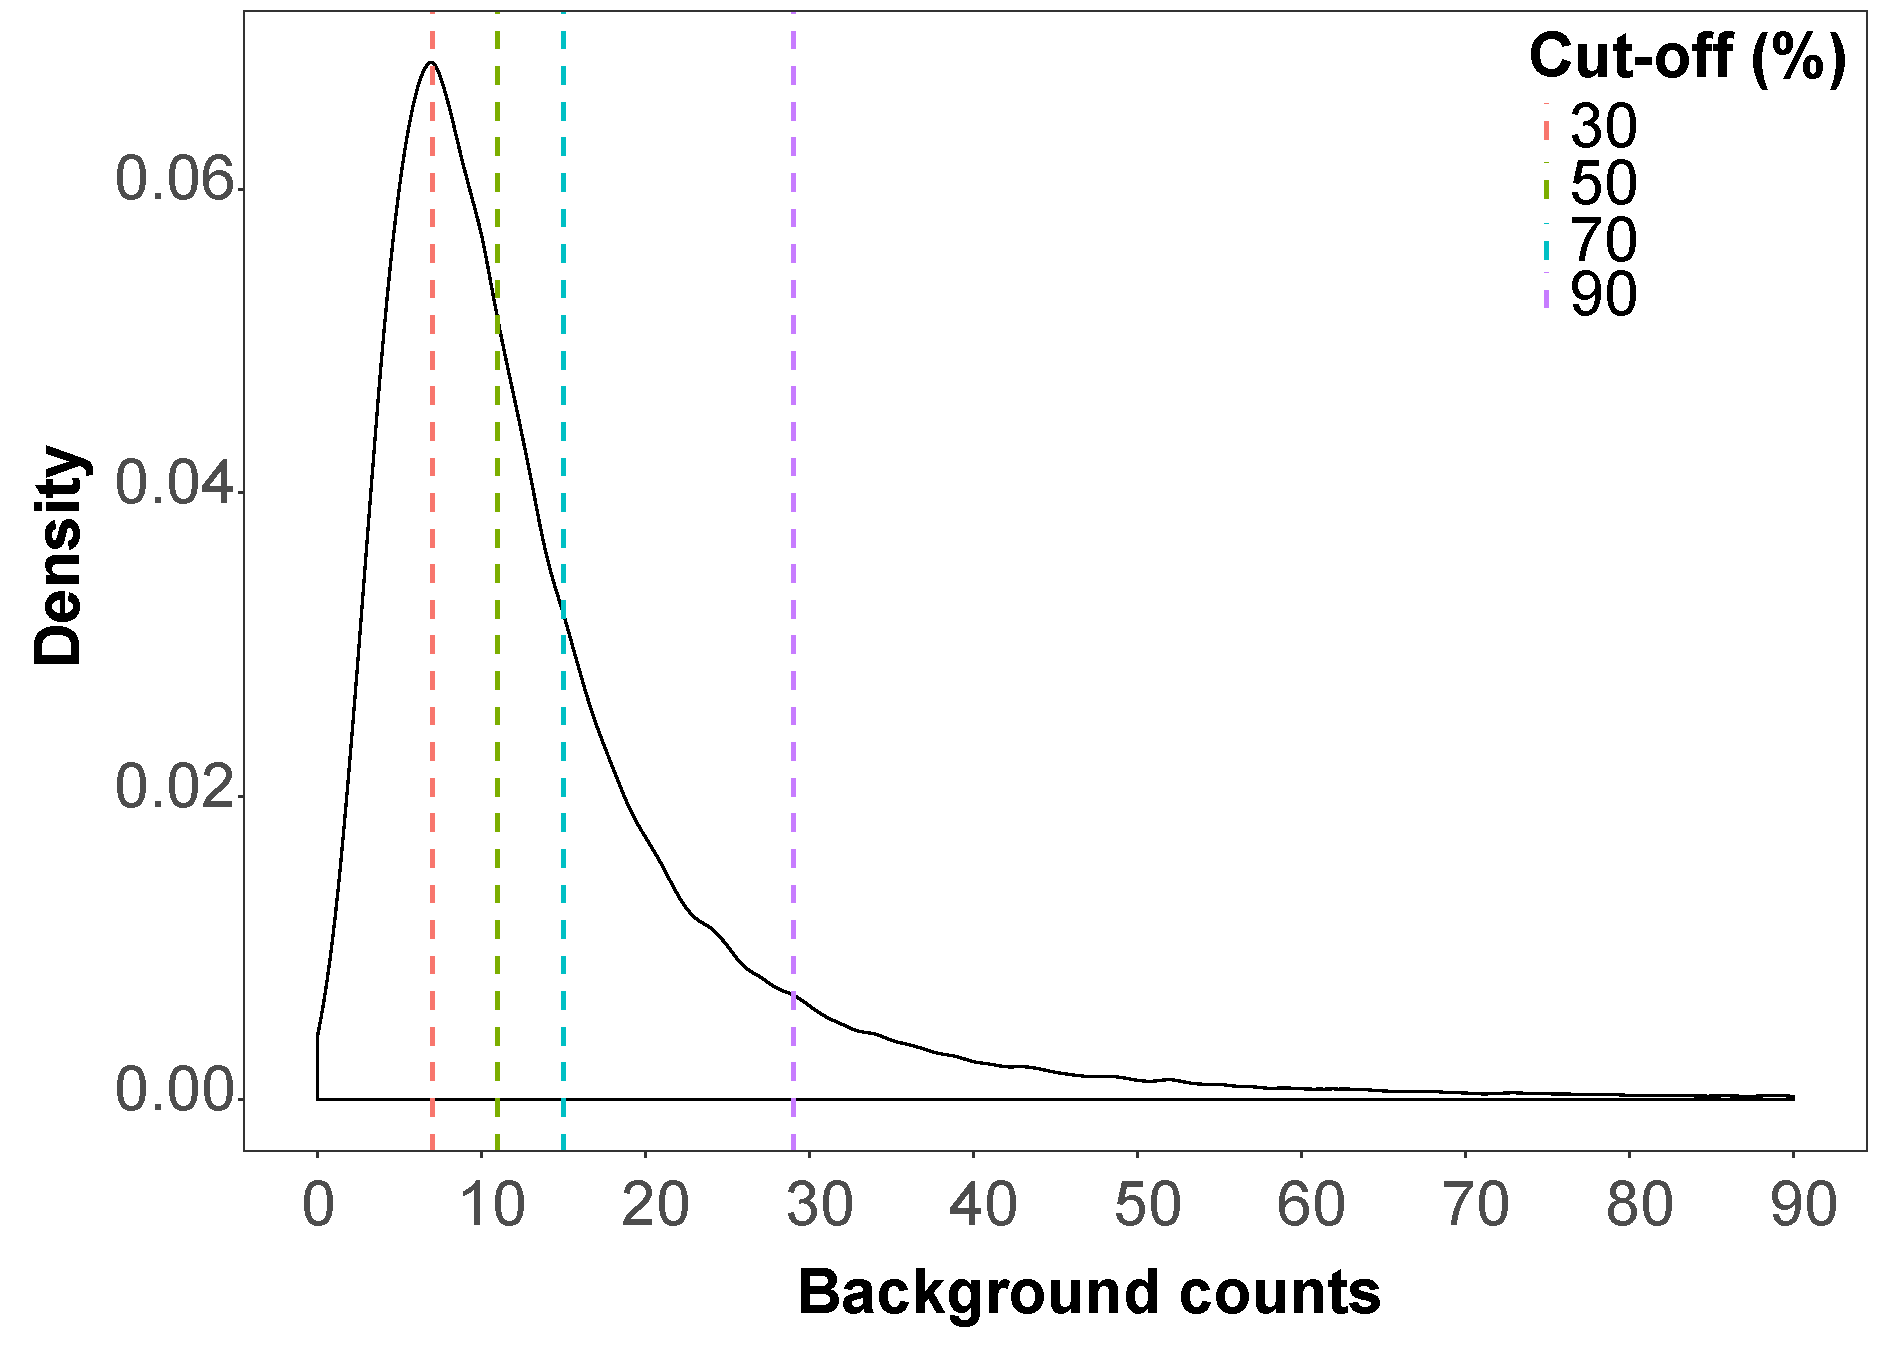
\includegraphics[width=0.5\textwidth]{./Appendix/pdfs/Chapter3/ATAC_absent_peaks_noise_distribution}
\caption[Distribution of the background read counts from all the master list peaks absent in each sample.]{\textbf{Distribution of the background read counts from all the master list peaks absent peaks in each sample.} Each cut-off corresponds to the number of background counts showed by a particular percentage of the total number of absent peaks.}
\label{figure:ATAC_absent_peaks_distribution}
\end{figure}


\begin{figure}[htbp]
\centering
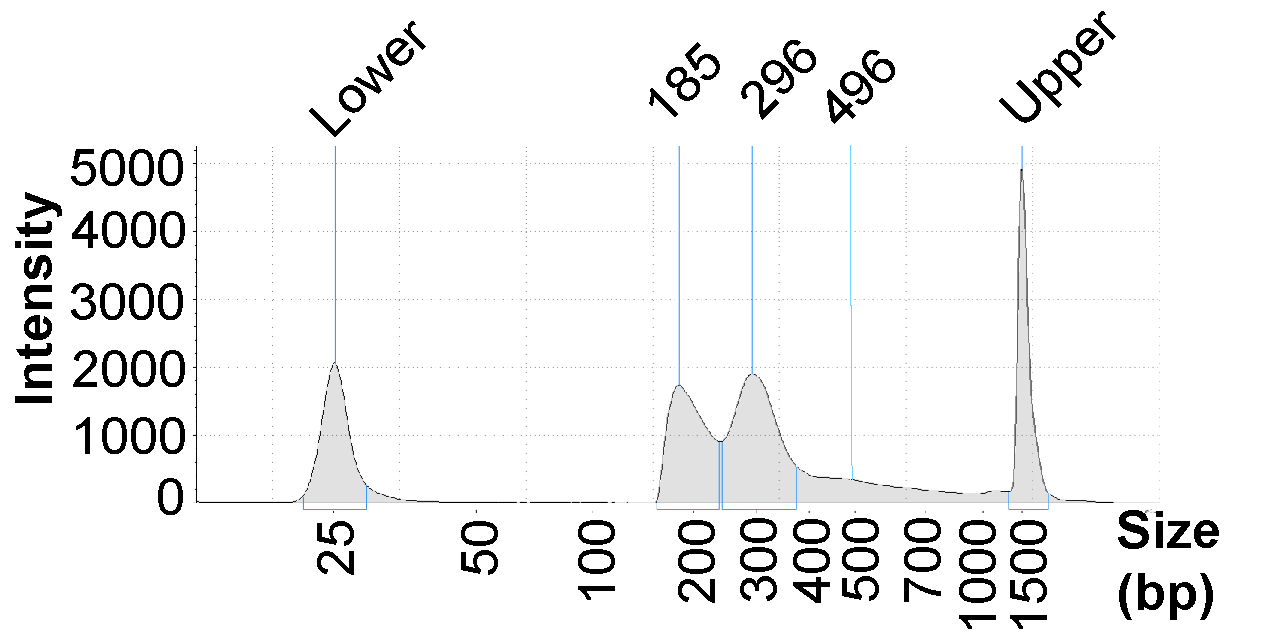
\includegraphics[width=0.5\textwidth]{./Appendix/pdfs/Chapter3/ATAC_PS02_tapestation_40min}
\caption[Pre-sequencing profiles of relative abundance of DNA library fragment sizes for a psoriatic lesional keratinocytes ATAC 1 library generated using 40 min of transposition.]{\textbf{Pre-sequencing profiles of relative abundance of DNA library fragment sizes for a psoriatic lesional keratinocytes ATAC 1 library generated using 40 min of transposition.} Pre-sequencing quantification of DNA fragment sizes from the ATAC library generated using 50,000 keratinocytes isolated from a psoriatic lesional skin biopsy and the ATAC 1 protocol (detailed in Table \ref{tab:ATAC_skin_optimisation_protocols}) and transposition for 40 min.}
\label{figure:PS2_40min_tapestation}
\end{figure}


\begin{figure}[htbp]
\centering
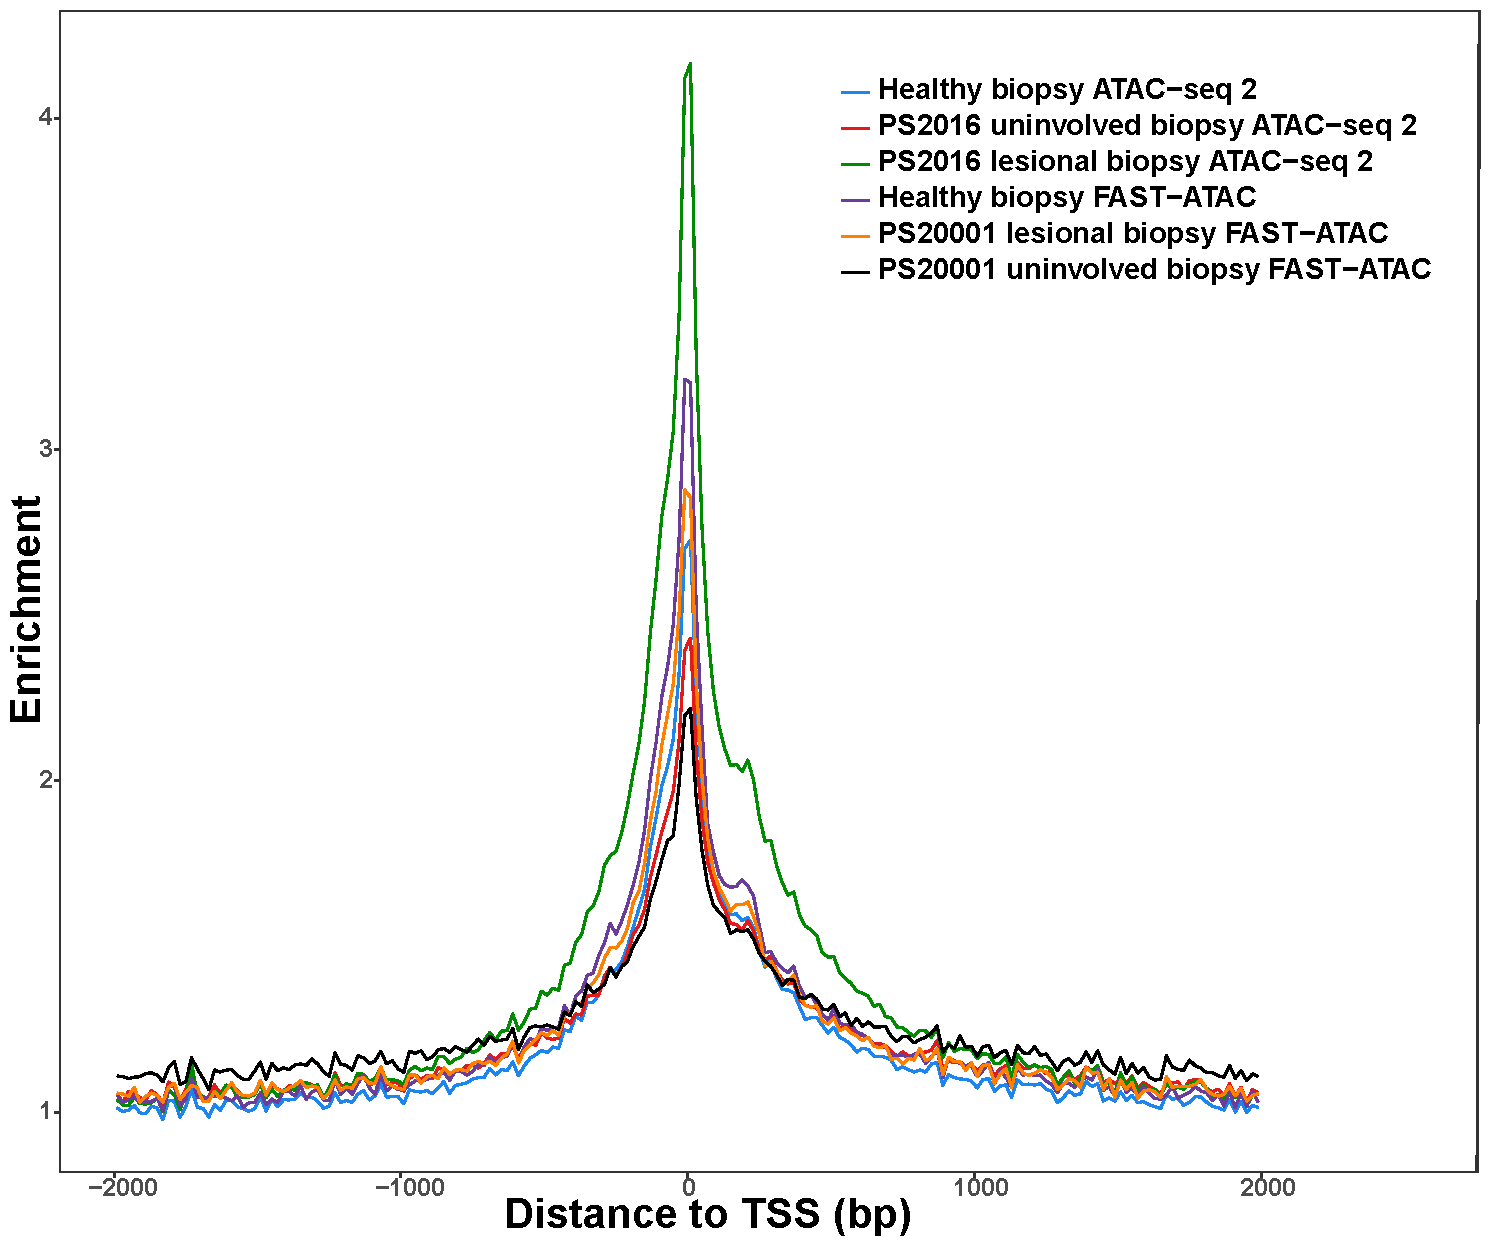
\includegraphics[width=0.5\textwidth]{./Appendix/pdfs/Chapter3/ATAC_skin_biopsy_samples_all_methods_TSS_enrichment_supplementary}
\caption[Assessment of TSS enrichment from ATAC 1 and Fast-ATAC in healthy and psoriasis KCs isolated from skin biopsy samples.]{\textbf{Assessment of TSS enrichment from ATAC 1 and Fast-ATAC in healthy and psoriasis KCs isolated from skin biopsy samples.} Fold-enrichment of ATAC fragments across the Ensembl annotated TSS from the different librariesgenerated using skin isolated keratinocytes from psoriasis patients (lesional and uninvolved) or healthy controls biopsies using ATAC 2 and Fast-ATAC protocols detailed in Table \ref{tab:ATAC_skin_optimisation_protocols}.}
\label{figure:TSS_skin_biopsies}
\end{figure}



\begin{figure}[htbp]
\centering
\begin{subfigure}{0.48\textwidth}
\centering
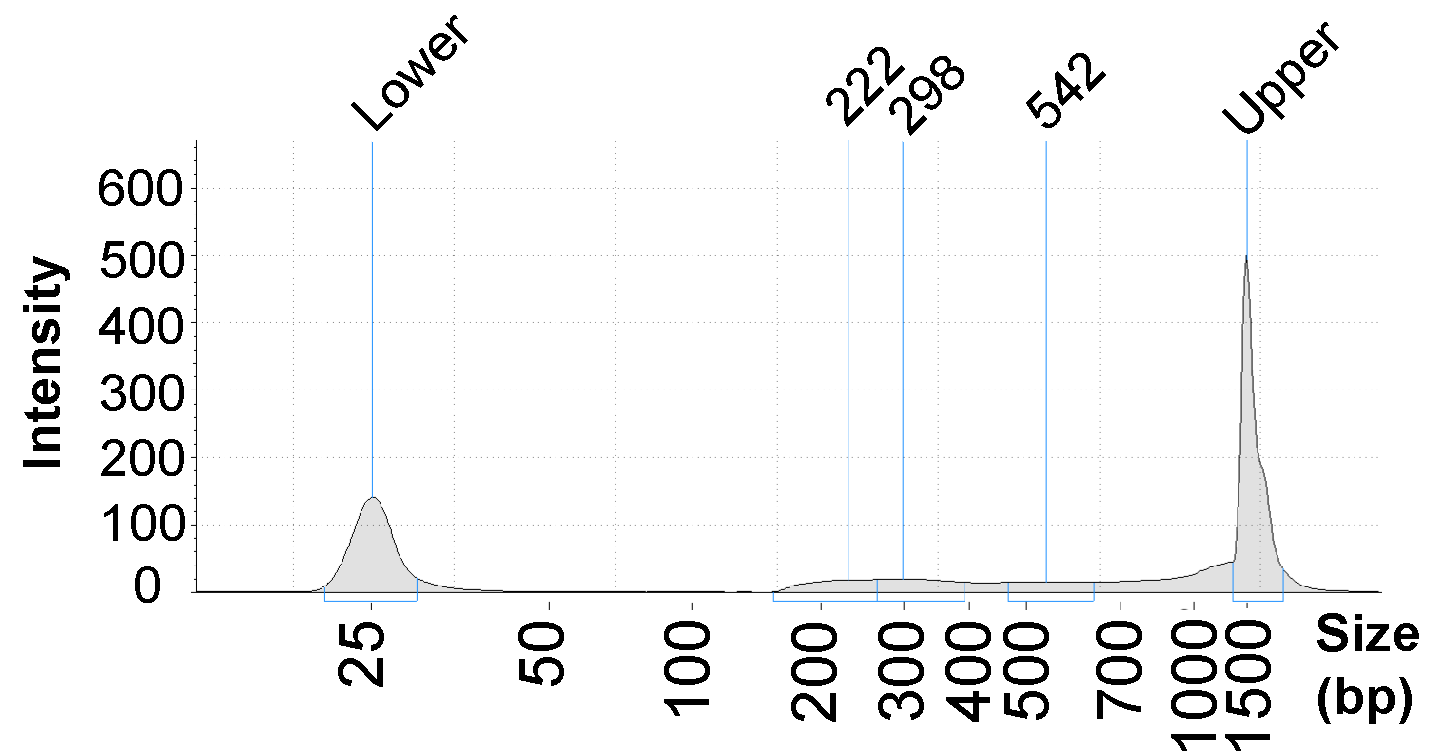
\includegraphics[width=\textwidth]{./Appendix/pdfs/Chapter3/FAST_ATAC_skin_tapestation_C1}
\caption{\textbf{}}
% The percentage sign indicated that the other subfig goes side by side
\end{subfigure}%
\begin{subfigure}{0.48\textwidth}
\centering
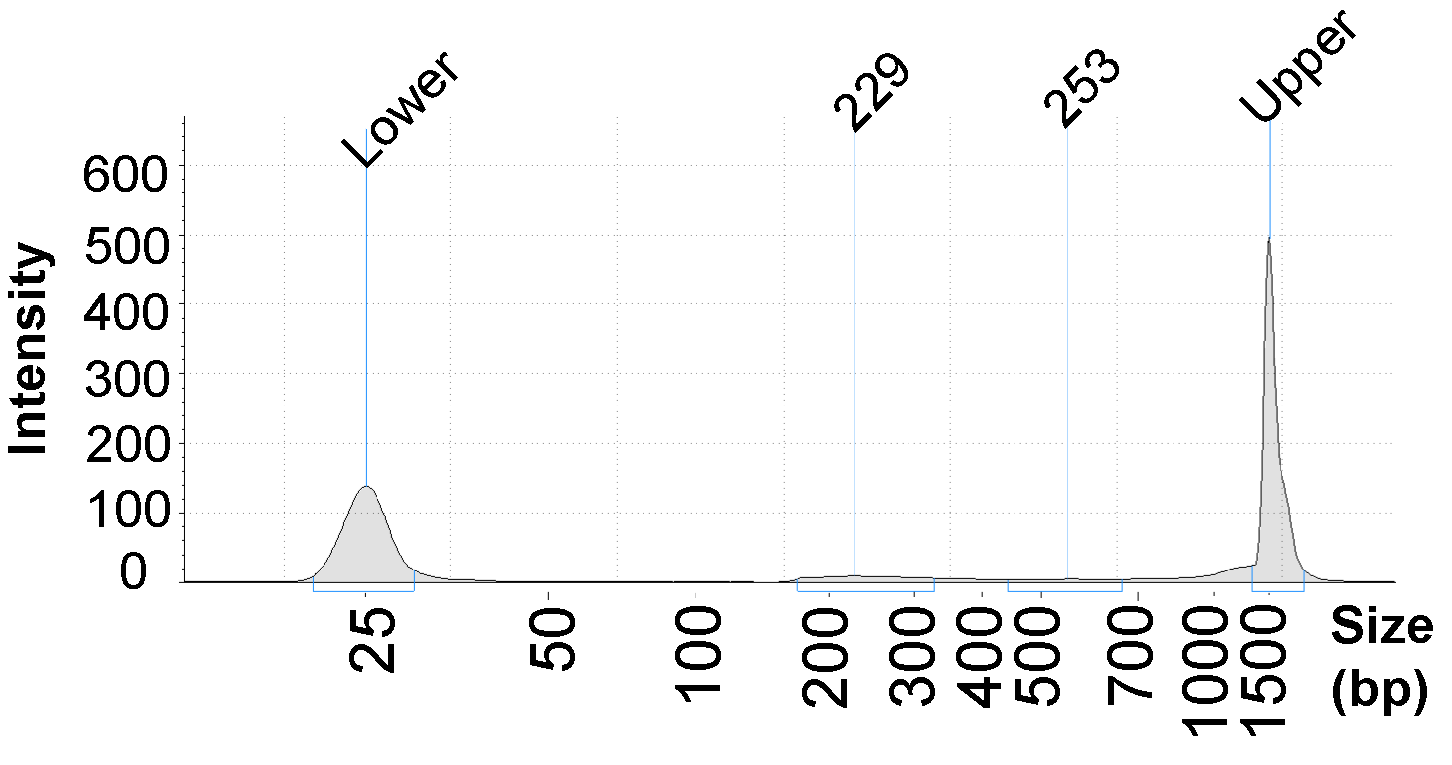
\includegraphics[width=\textwidth]{./Appendix/pdfs/Chapter3/FAST_ATAC_skin_tapestation_C3}
\caption{\textbf{}}
\end{subfigure}
\begin{subfigure}{0.48\textwidth}
\centering
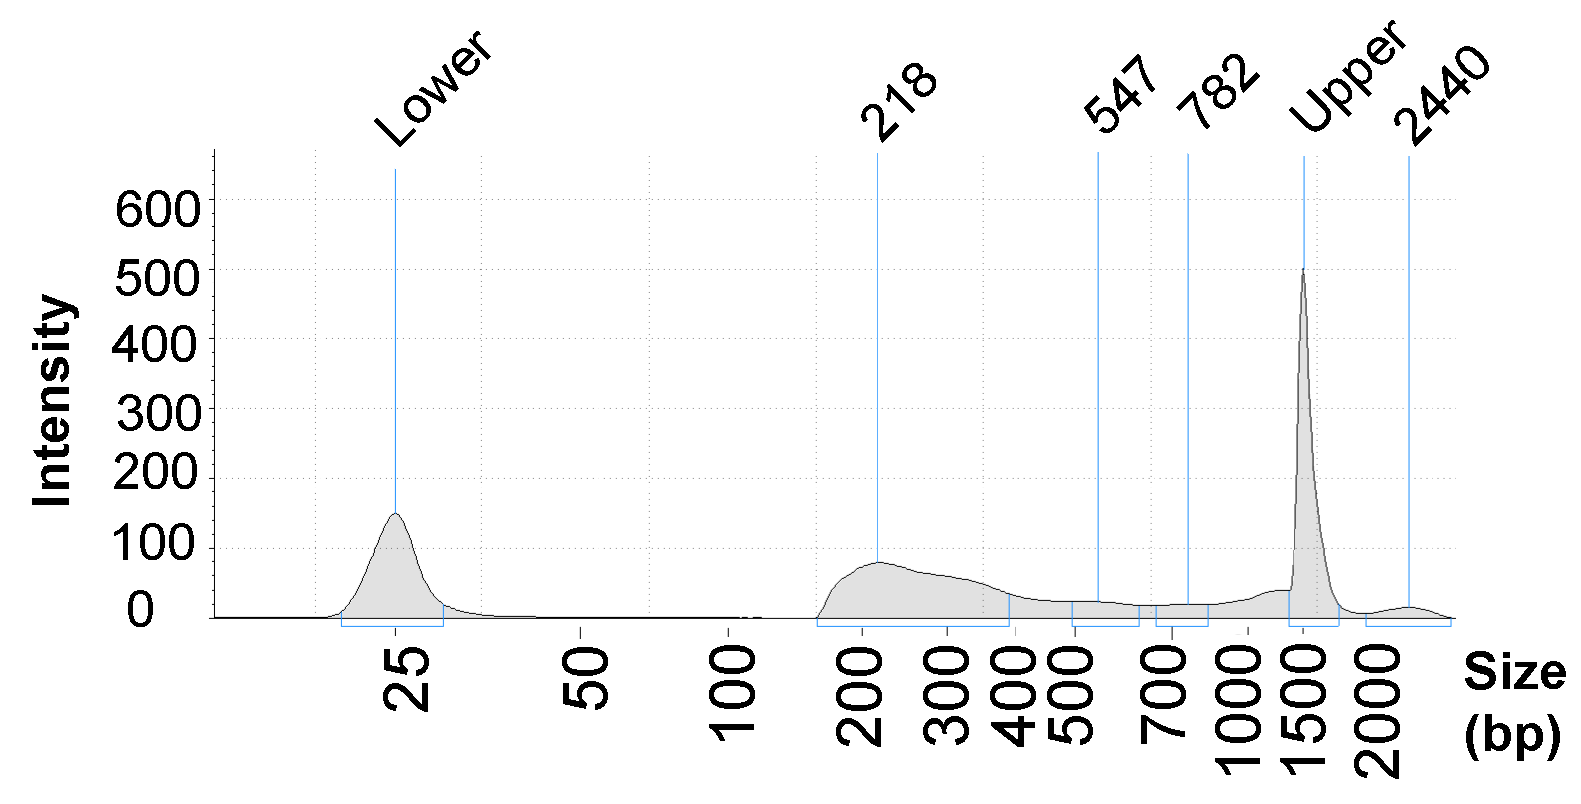
\includegraphics[width=\textwidth]{./Appendix/pdfs/Chapter3/FAST_ATAC_skin_tapestation_C4}
\caption{\textbf{}} % to add text to the figure name
\end{subfigure}%
\begin{subfigure}{0.48\textwidth}
\centering
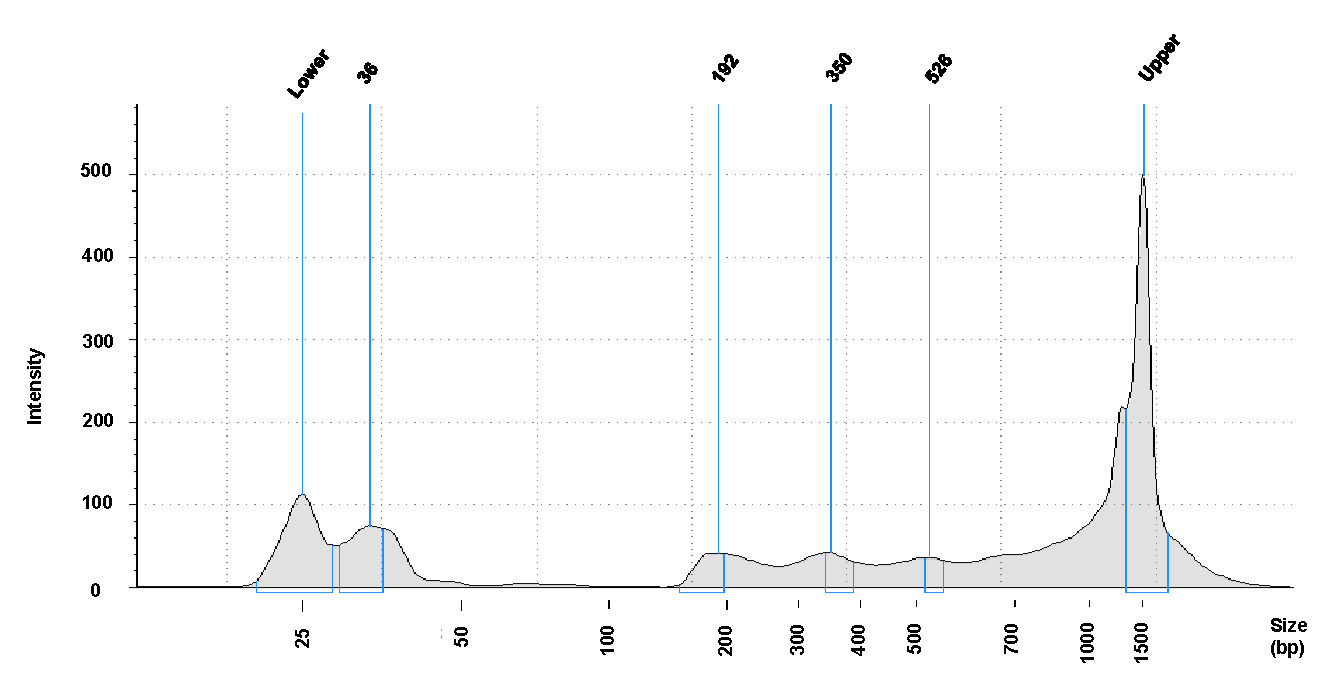
\includegraphics[width=\textwidth]{./Appendix/pdfs/Chapter3/Omni_ATAC_NHEK_Rep1_tapestation}
\caption{\textbf{}} % to add text to the figure name
\end{subfigure}
\hfill
\caption[Fast-ATAC and Omni-ATAC NHEK pre-sequencing profiles of relative abundance of DNA library fragment sizes.]{\textbf{Fast-ATAC and Omni-ATAC NHEK pre-sequencing profiles of relative abundance of DNA library fragment sizes.} Pre-sequencing quantification of DNA fragment sizes from the libraries generated  using the (A) C2, (B) C3, and (C) C4 versions of the Fast-ATAC protocol based on modifications in the detergent and Tn5 concentration and (D) Omni-ATAC. C2, C3 and C4 detergent and Tn5 concentrations are detailed in Table \ref{tab:ATAC_skin_optimisation_protocols}.}
\label{figure:NHEK_tapestation}
\end{figure}


\bigskip
\begin{figure}[t]
	\centering
	\begin{subfigure}[b]{0.48\textwidth}
		\centering 
		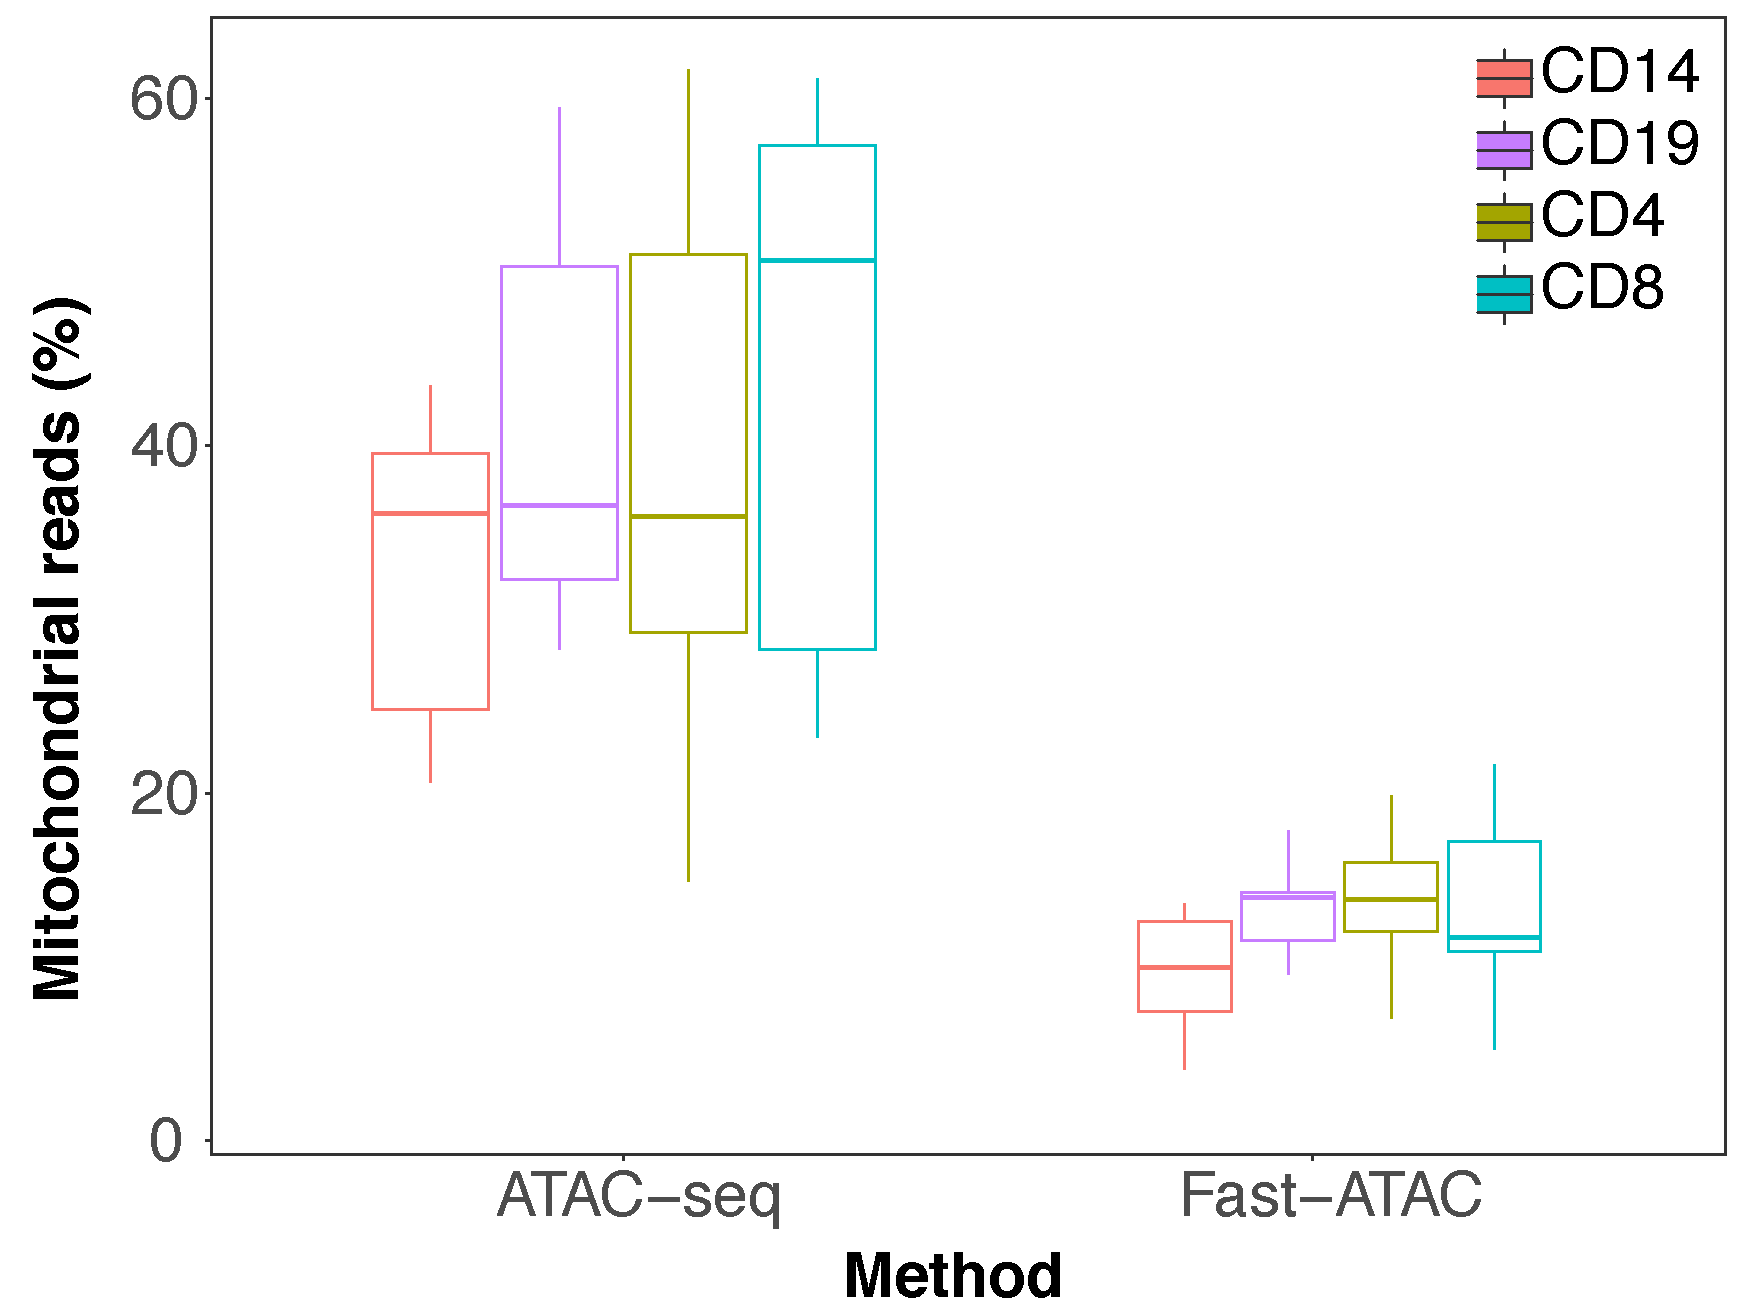
\includegraphics[width=\textwidth]{./Appendix/pdfs/Chapter3/ATAC_all_samples_MT_by_method_and_cell_type}
		\caption{}
	\end{subfigure}%
	~
	\begin{subfigure}[b]{0.48\textwidth} 
		%the [b] prevents offset in subcaptions
		\centering
		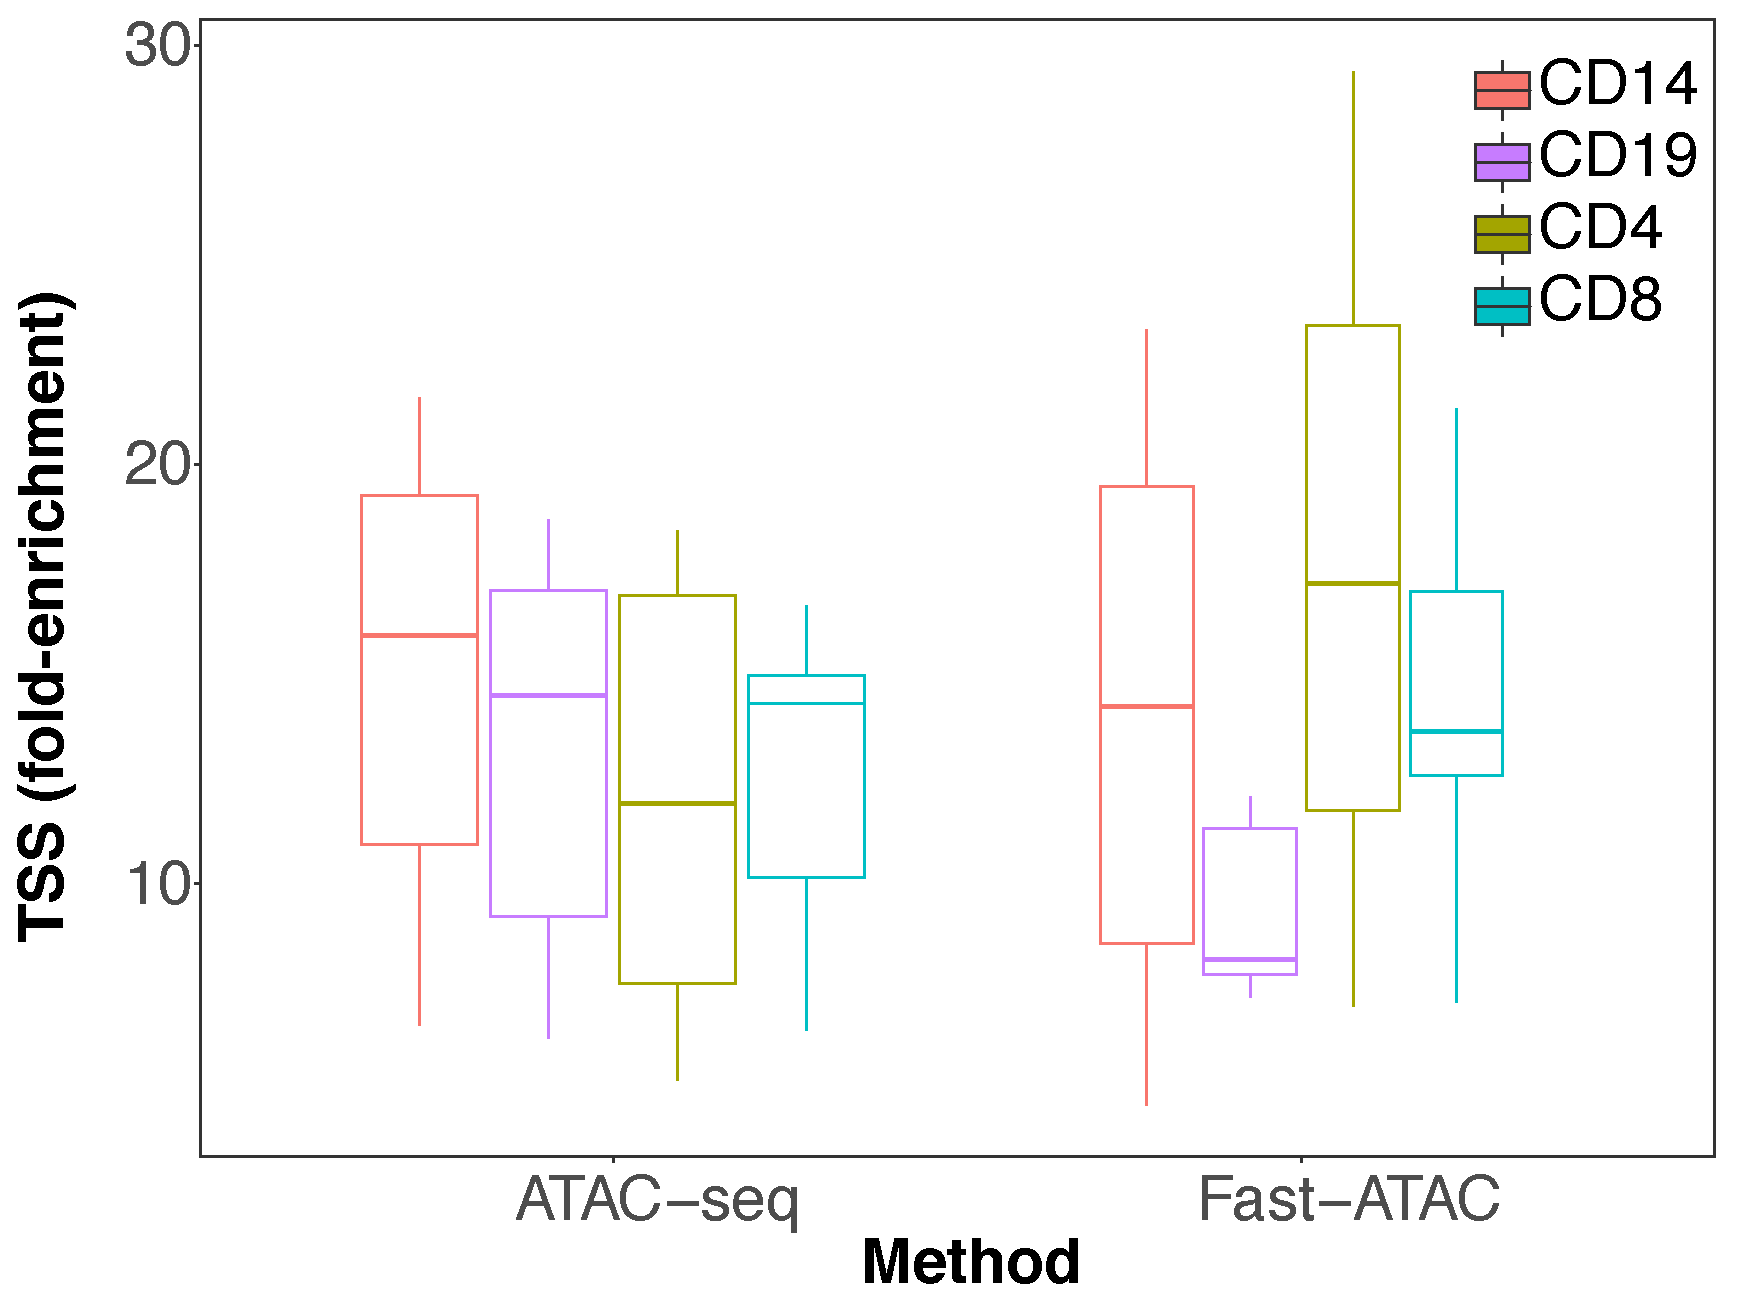
\includegraphics[width=\textwidth]{./Appendix/pdfs/Chapter3/ATAC_all_samples_TSS_by_method_and_cell_type}%
		\caption{}
	\end{subfigure}
	\caption[Differences in TSS fold-enrichment and percentage of mitochondrial between the ATAC-seq and Fast-ATAC libraries from all the samples generated in the thesis.]{\textbf{Differences in TSS fold-enrichment and percentage of mitochondrial between the ATAC-seq and Fast-ATAC libraries from all the samples generated in the thesis.} Boxplox illustrating differences between ATAC-seq and Fast-ATAC by cell type for (A) TSS fold enrichment and (B) mitochondrial reads (percentage).}
	\label{figure:Comparison_ATACseq_vs_fastATAC_all_thesis_samples}
\end{figure}



\clearpage


\section{Chapter 4 Figures}

\begin{figure}[htbp]
\centering
\begin{subfigure}{0.45\textwidth}
\centering
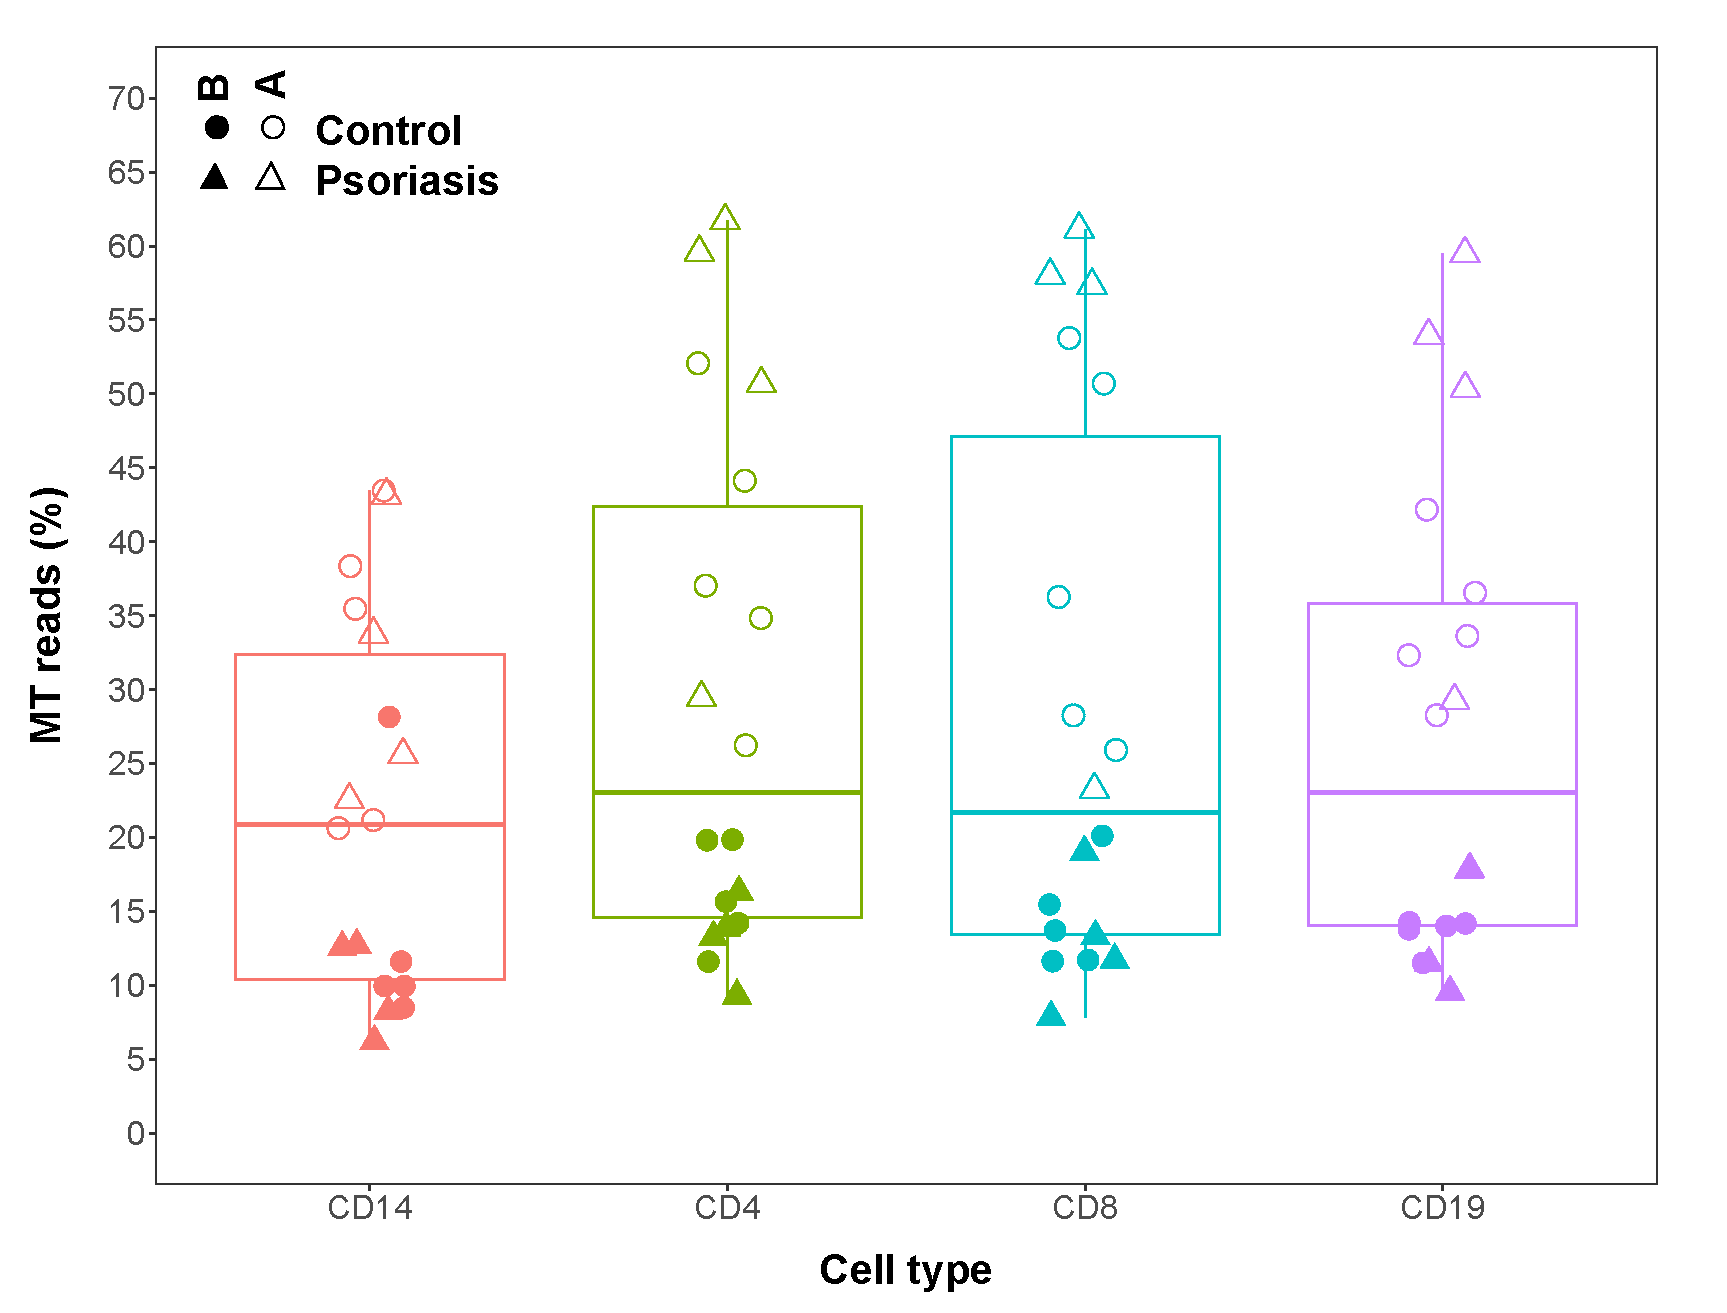
\includegraphics[width=\textwidth]{./Appendix/pdfs/Chapter4/ATAC_PS_CTL_MT_percent_boxplot}
\caption{\textbf{}}
\end{subfigure}
\begin{subfigure}{0.45\textwidth}
\centering
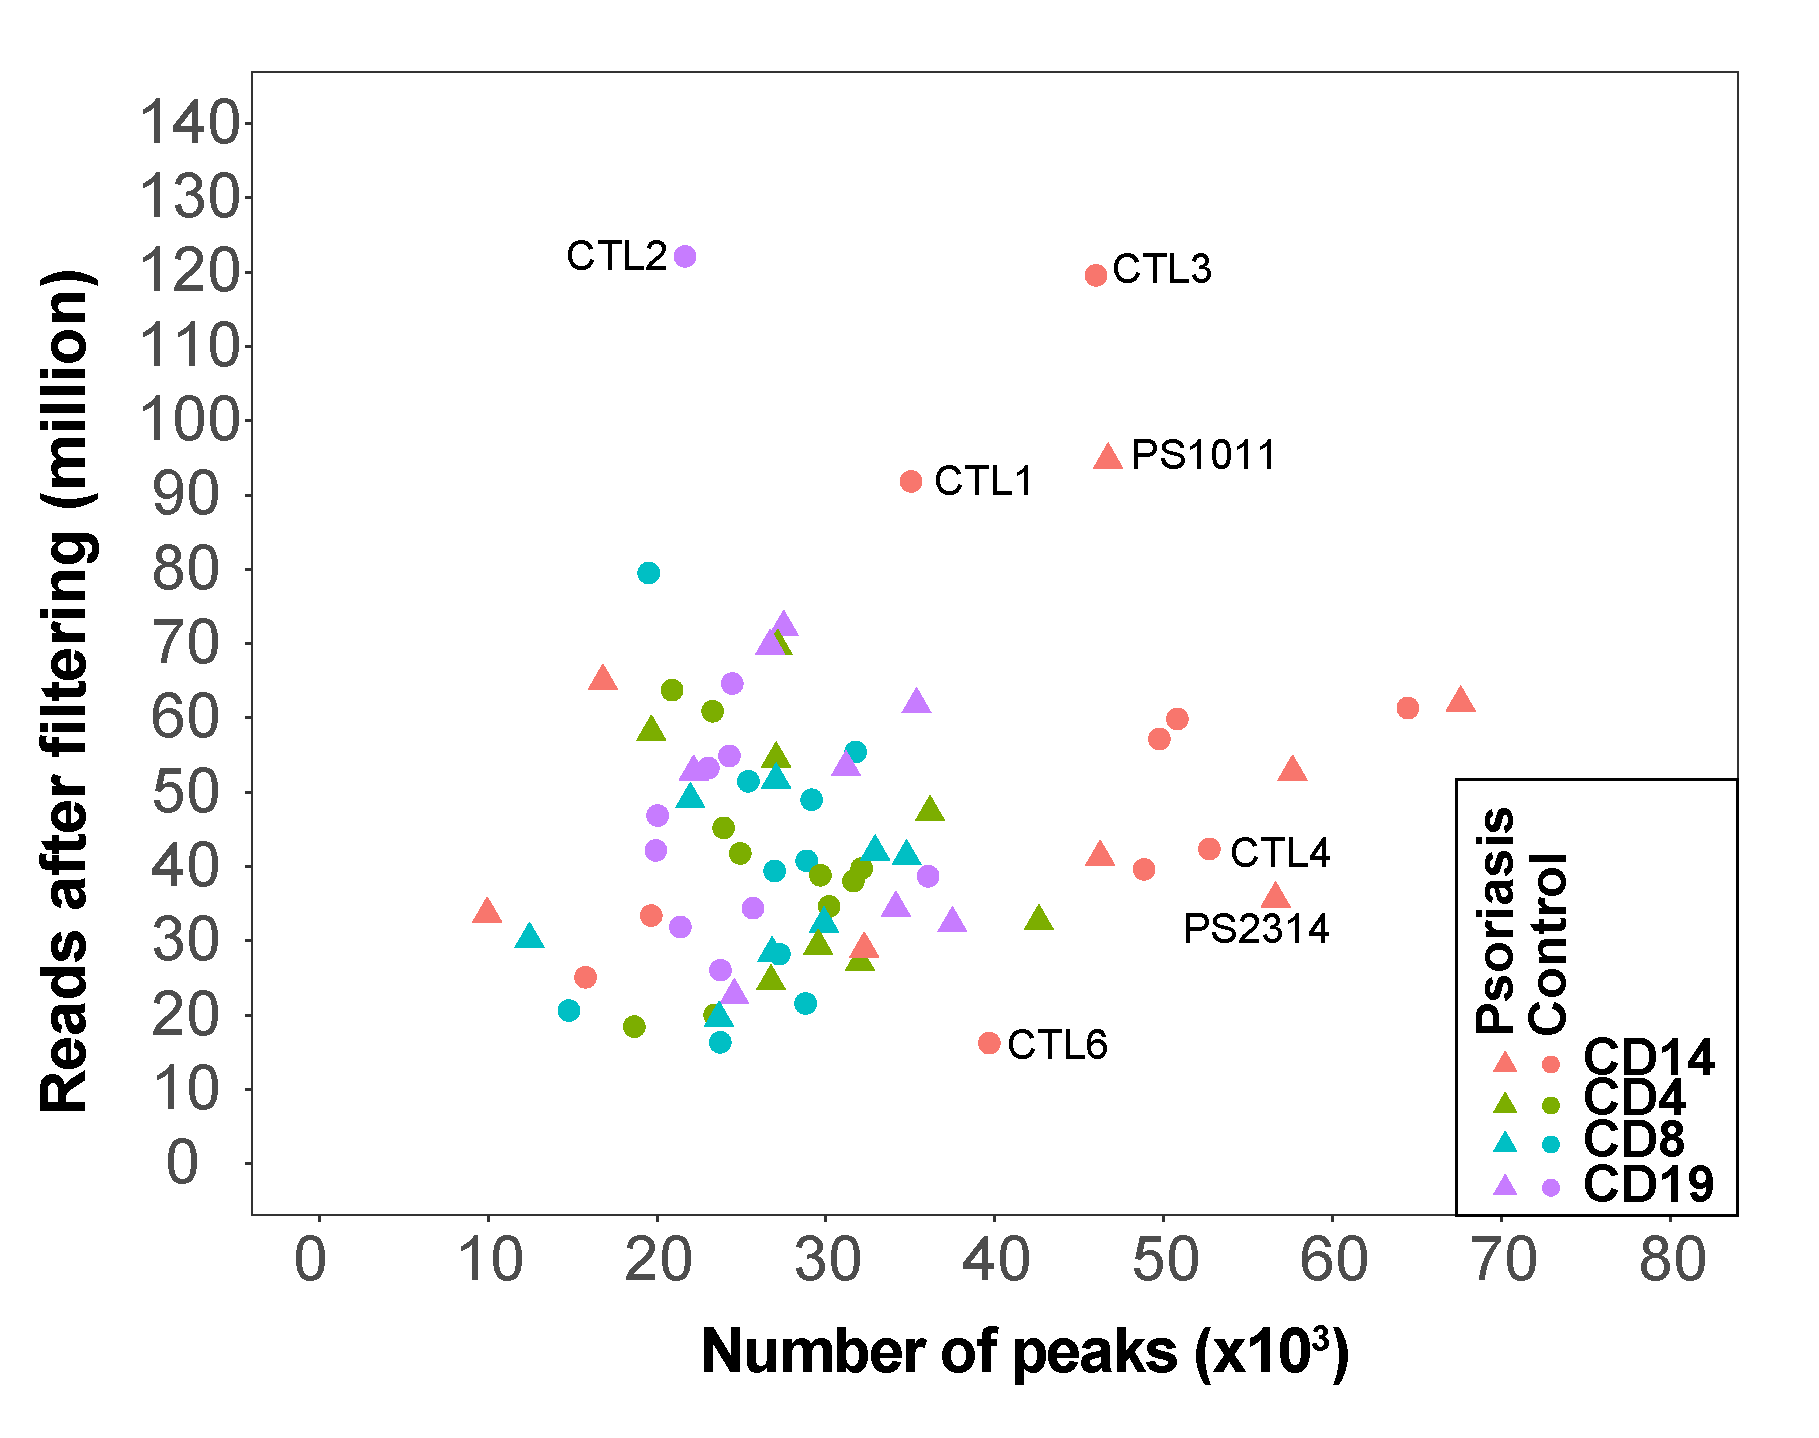
\includegraphics[width=\textwidth]{./Appendix/pdfs/Chapter4/ATAC_PS_CTL_reads_vs_peaks_dotplot}
\caption{\textbf{}}
\end{subfigure}
\caption[Mitochondrial reads and called peaks after IDR p-value filtering in the ATAC libraries generated in psoriasis patients and healthy control samples.]{\textbf{Miitochondrial reads and called peaks after IDR p-value filtering in the ATAC libraries generated in psoriasis patients and healthy control samples.}. (A) Percentage of MT reads in the ATAC-seq samples generated in CD14$^+$ monocytes, CD4$^+$, CD8$^+$ and CD19$^+$ isolated from psoriasis patients and healthy controls. Samples from cohort 1A (open circles and triangles) were generated with the standard ATAC-seq protocol from Buenrostro \textit{et al.}, 2013 whereas samples from cohort 1B (filled circles and triangles) were processed using FAST-ATAC \parencite{Corces2016}. (B) For each of the ATAC libraries, representation of the number of significant peaks based on IDR optimal p-value filtering versus the total million of reads after filtering.}
\label{figure:ATAC_PS_CTL_MT_percent_and_called_peaks}
\end{figure}


%\begin{figure}[htbp]
%\centering
%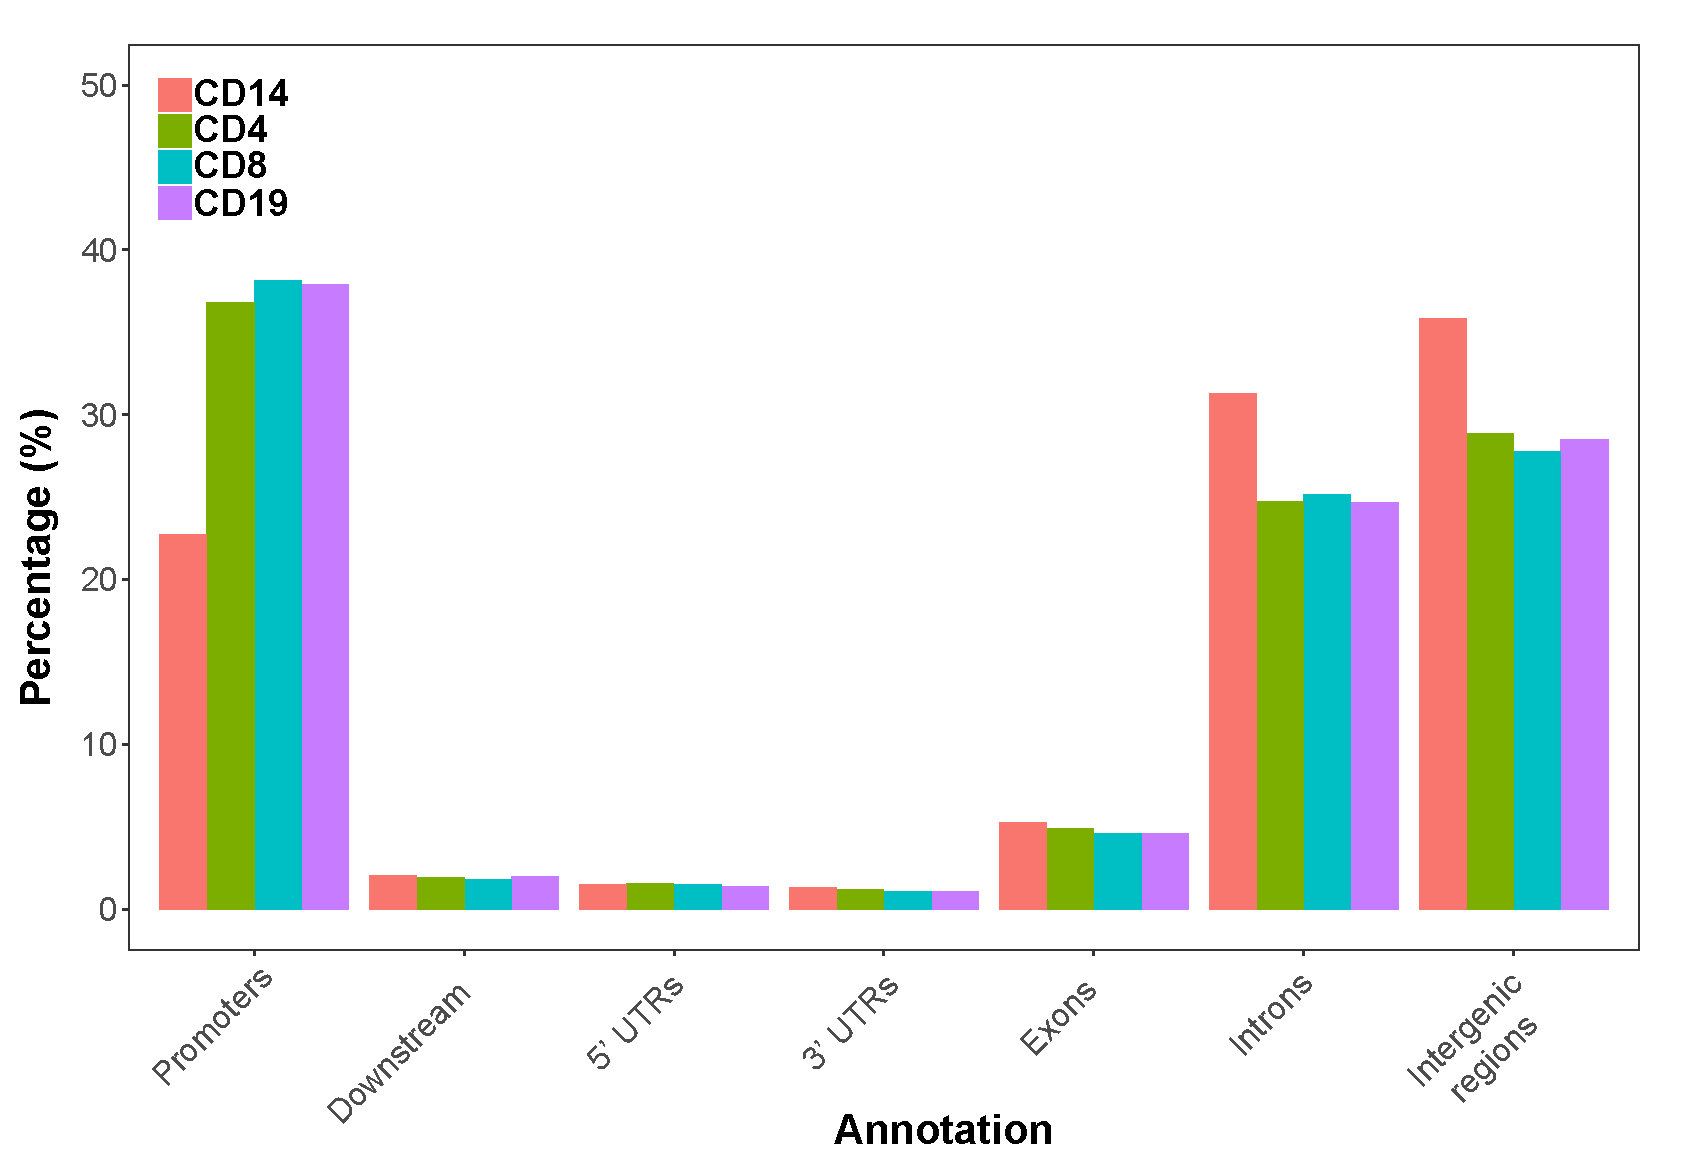
\includegraphics[width=0.6\textwidth]{./Appendix/pdfs/Chapter4/ATAC_all_cell_types_individual_master_lists_general_peak_annotation}
%\caption[Genomic annotation of the consensus master list of ATAC-seq enriched sites built for downstream differential chromatin accessibility analysis in CD14$^+$ monocytes, CD4$^+$, CD8$^+$ and CD19$^+$.]{\textbf{Genomic annotation of the consensus master list of ATAC-seq enriched sites built for downstream differential chromatin accessibility analysis in CD14$^+$ monocytes, CD4$^+$, CD8$^+$ and CD19$^+$.} Annotation is expressed in percentage over the total number of ATAC-seq sites included in each particular cell type master list.}
%\label{fig:ATAC_PS_CTL_genomic_annotation}
%\end{figure}


\bigskip
\begin{figure}[htbp]
\centering
\begin{subfigure}[b]{0.45\textwidth}
\centering 
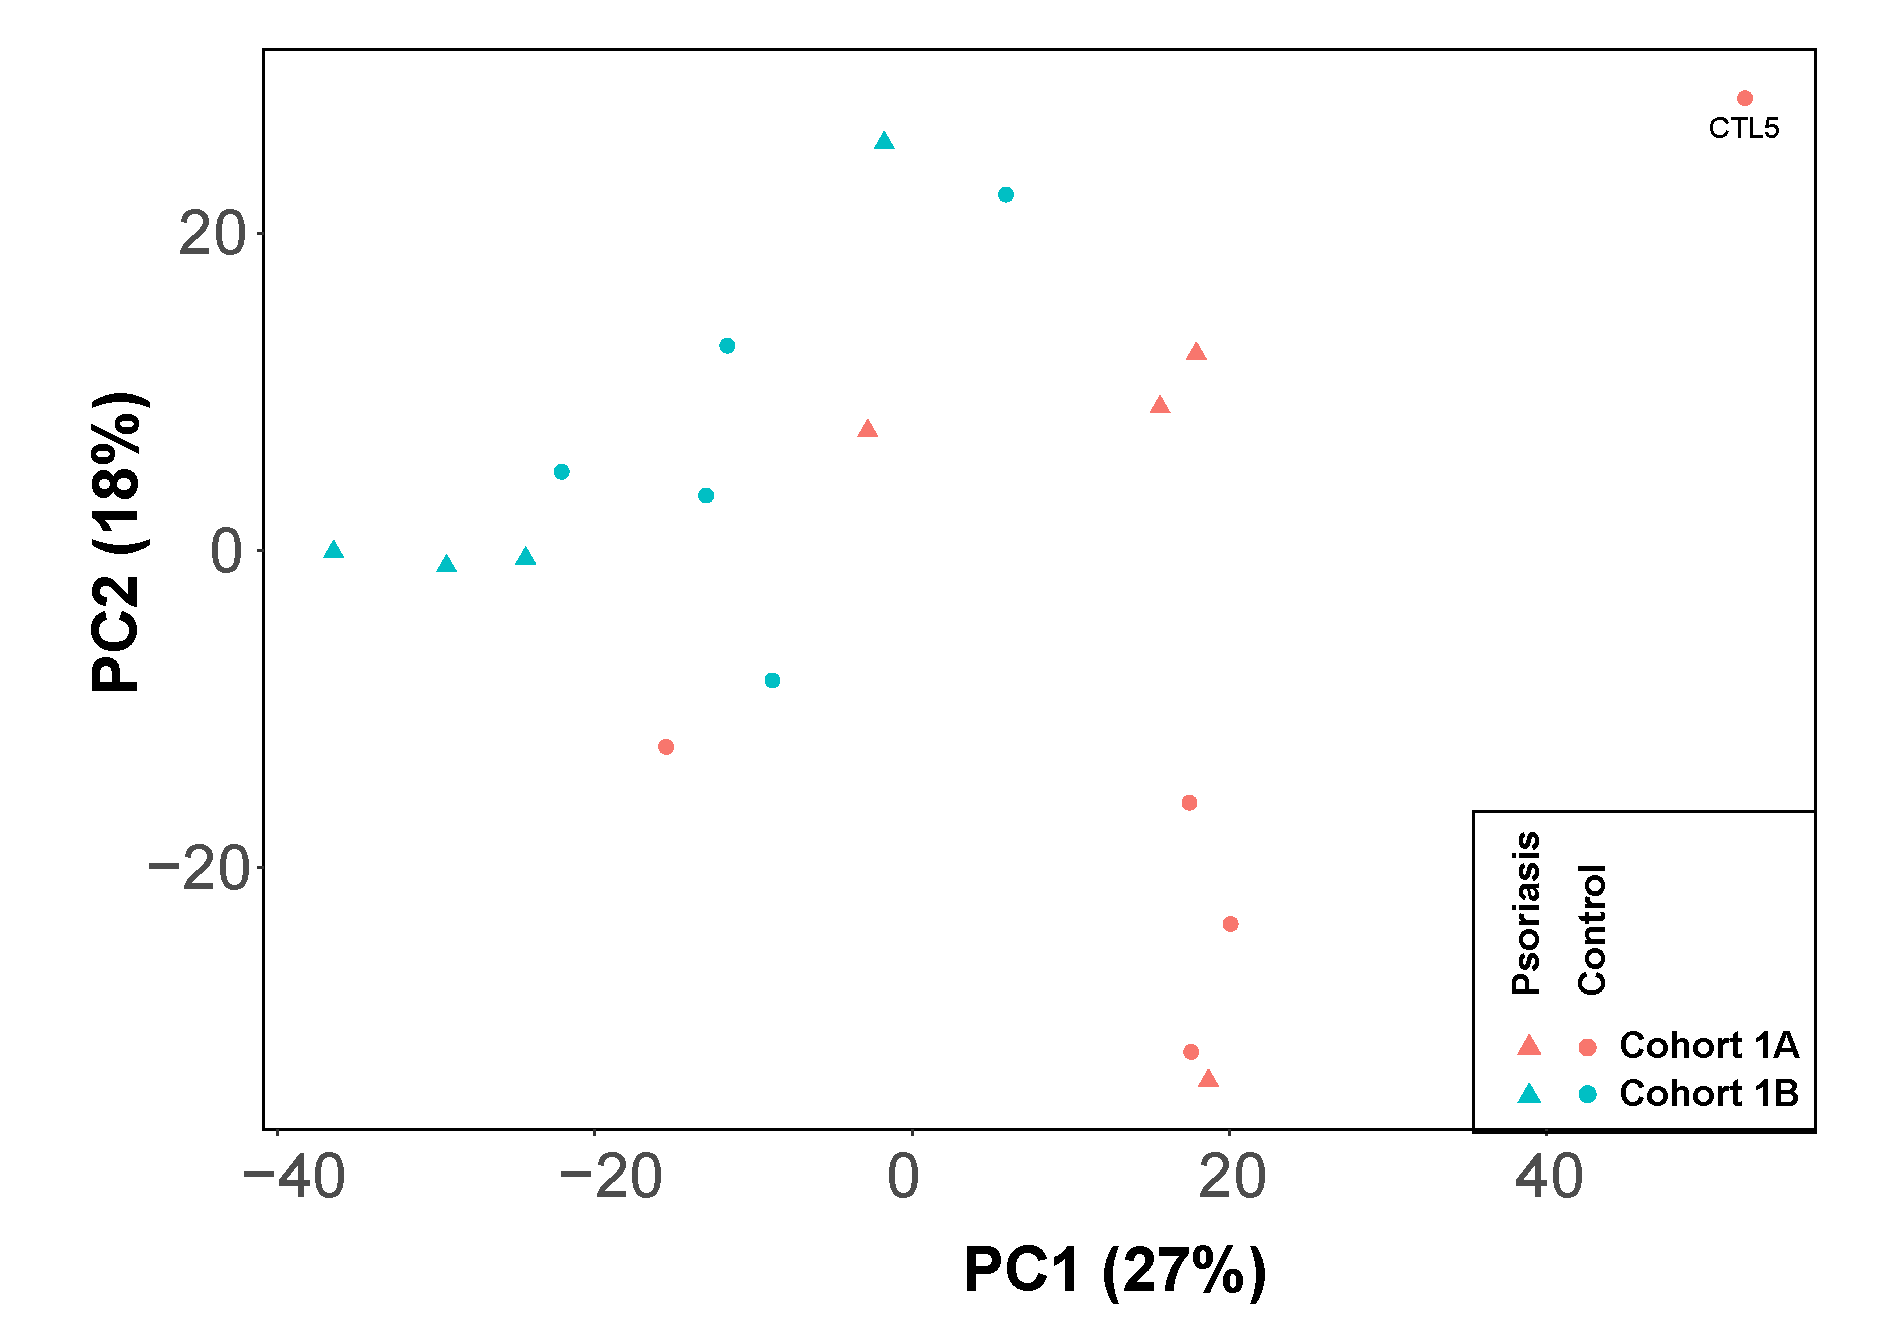
\includegraphics[width=\textwidth]{./Appendix/pdfs/Chapter4/ATAC_CD8_PS_CTL_PCA}
\caption{}
\end{subfigure}%
~
\begin{subfigure}[b]{0.45\textwidth} 
%the [b] prevents offset in subcaptions
\centering
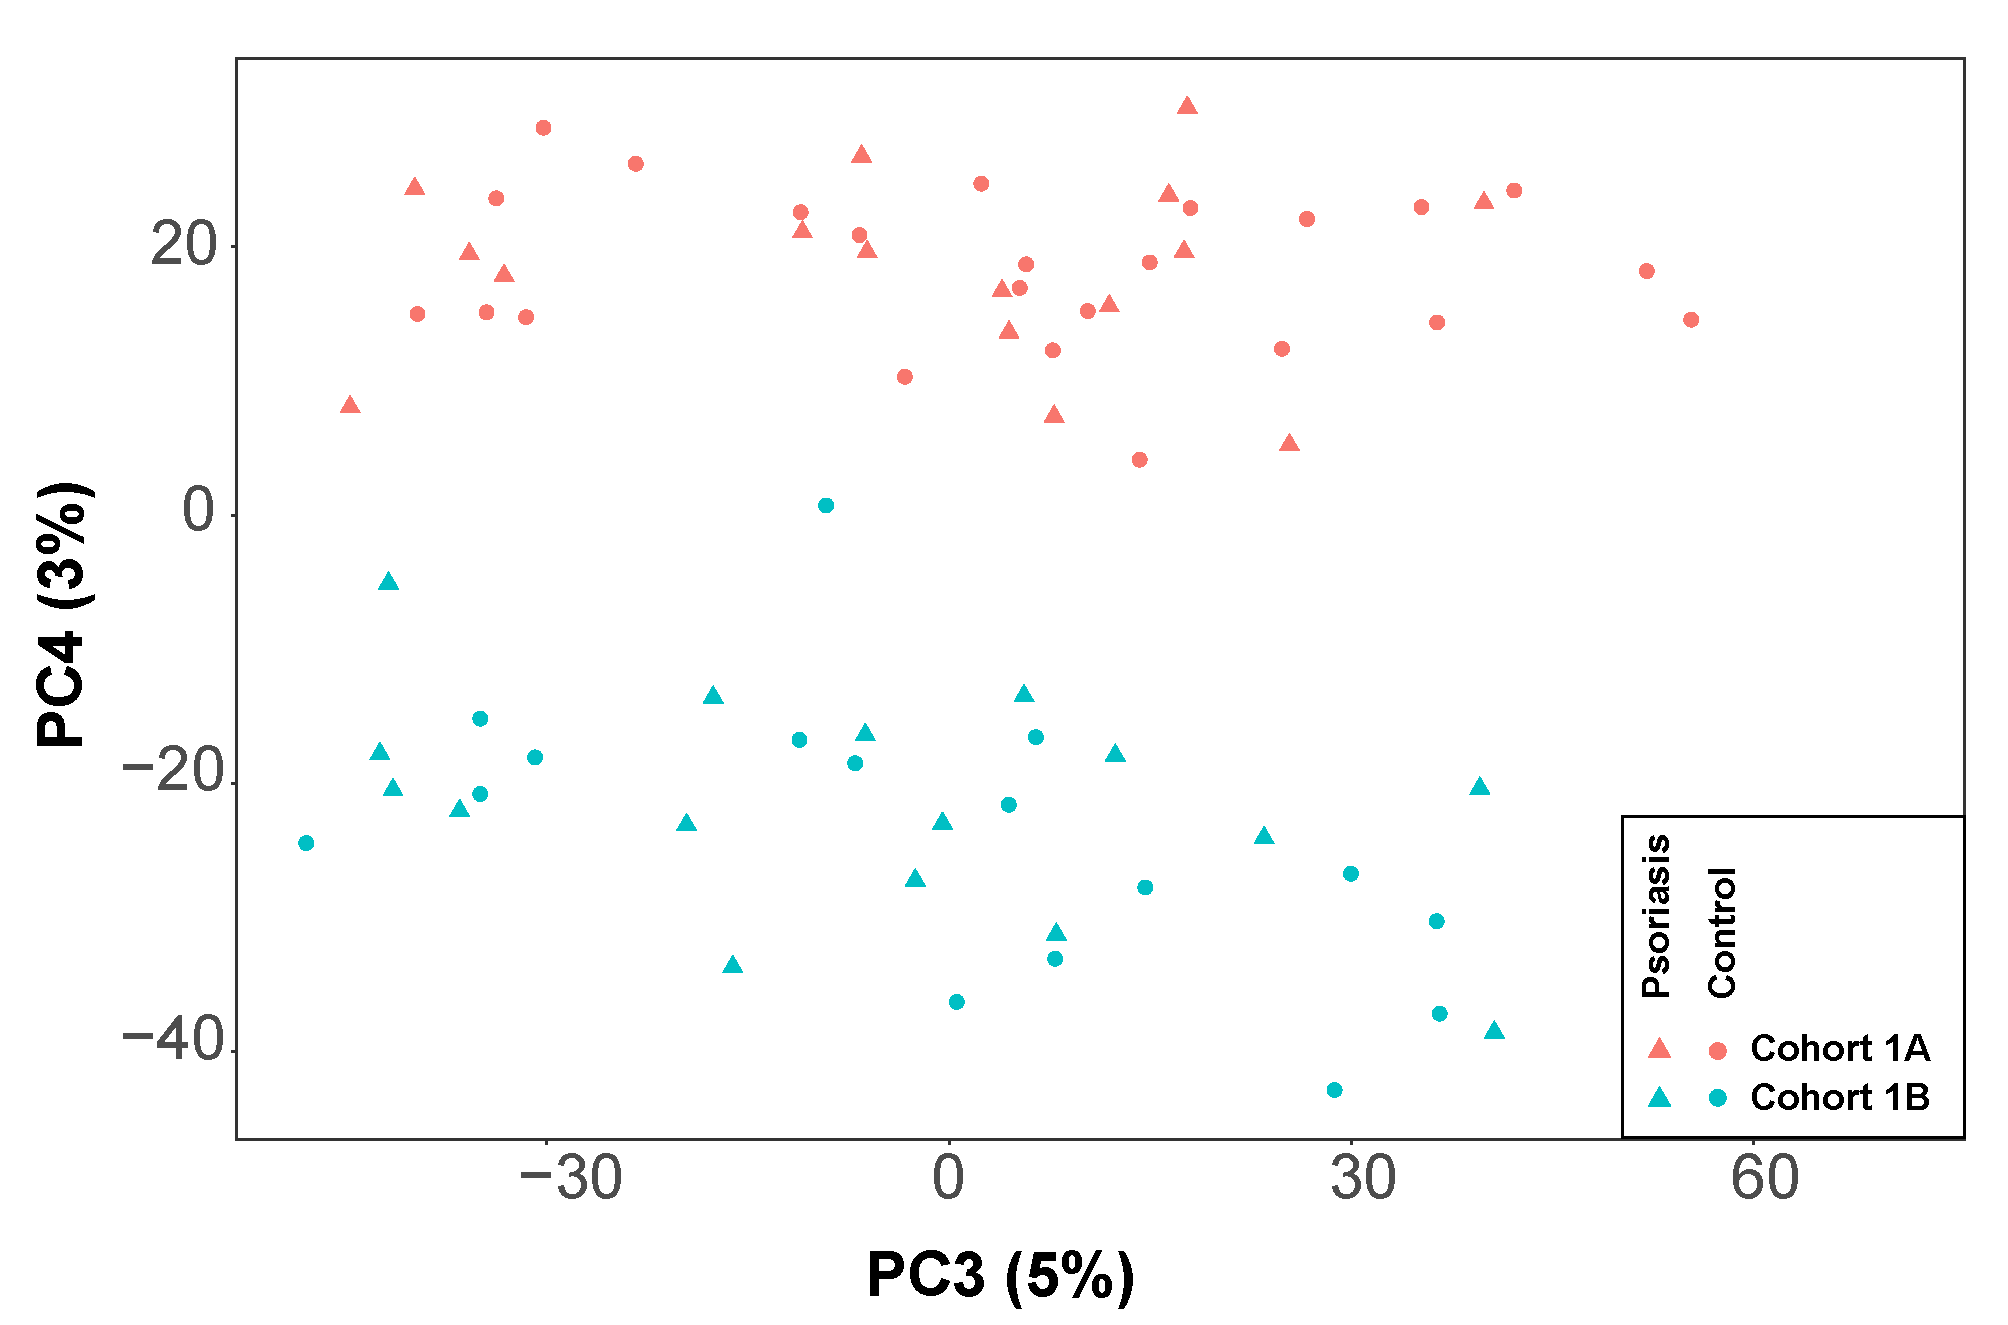
\includegraphics[width=\textwidth]{./Appendix/pdfs/Chapter4/PS_CTL_all_samples_varied_PCA3and4_plot}
\caption{}
\end{subfigure}
\caption[PCA analysis illustrating batch effect in ATAC and RNA-seq samples.]{\textbf{PCA analysis illustrating batch effect in ATAC and RNA-seq samples.} (A) First and second component of the PCA analysis performed using the normalised ATAC counts in a list of consensus peaks across all the combined CD8$^+$ samples from psoriasis patients and healthy controls. (B) Third and fourth component of the PCA analysis performed on the normalised number of reads mapping to the Ensmbl list of mRNAs and lncRNAs detected in CD8$^+$ cells from psoriasis patients and healthy controls.}
\label{figure:ATAC_RNAseq_batch_effect}
\end{figure}



\begin{figure}[htbp]
\centering
\begin{subfigure}{0.45\textwidth}
\centering
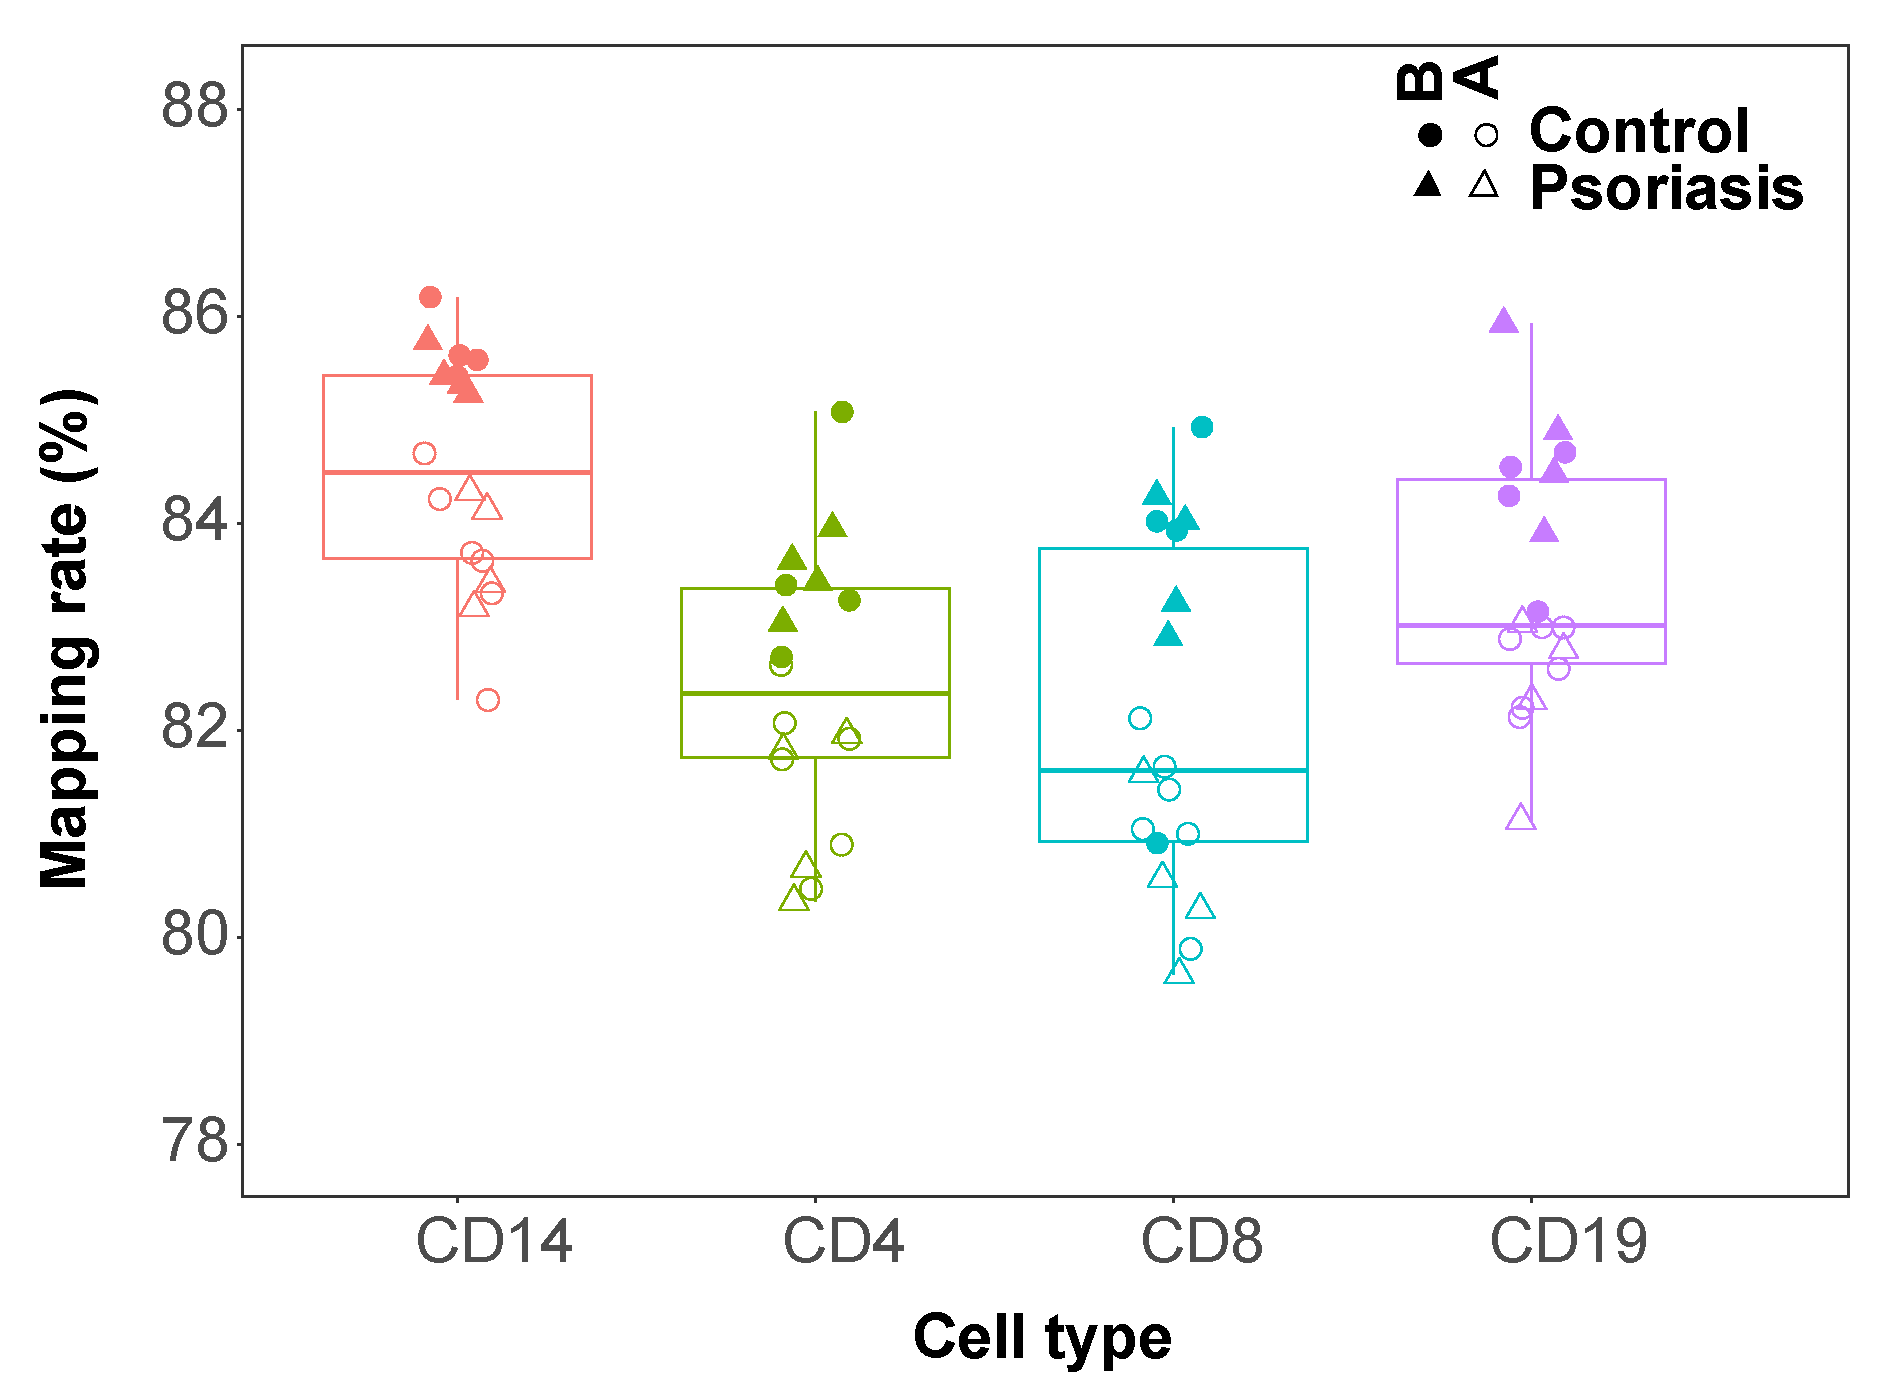
\includegraphics[width=\textwidth]{./Appendix/pdfs/Chapter4/PS_CTL_RNAseq_uniquely_mapped_reads_rate_cell_type_batch_and_condition_boxplots}
\caption{\textbf{}}
% The percentage sign indicated that the other subfig goes side by side
\end{subfigure}%
\begin{subfigure}{0.45\textwidth}
\centering
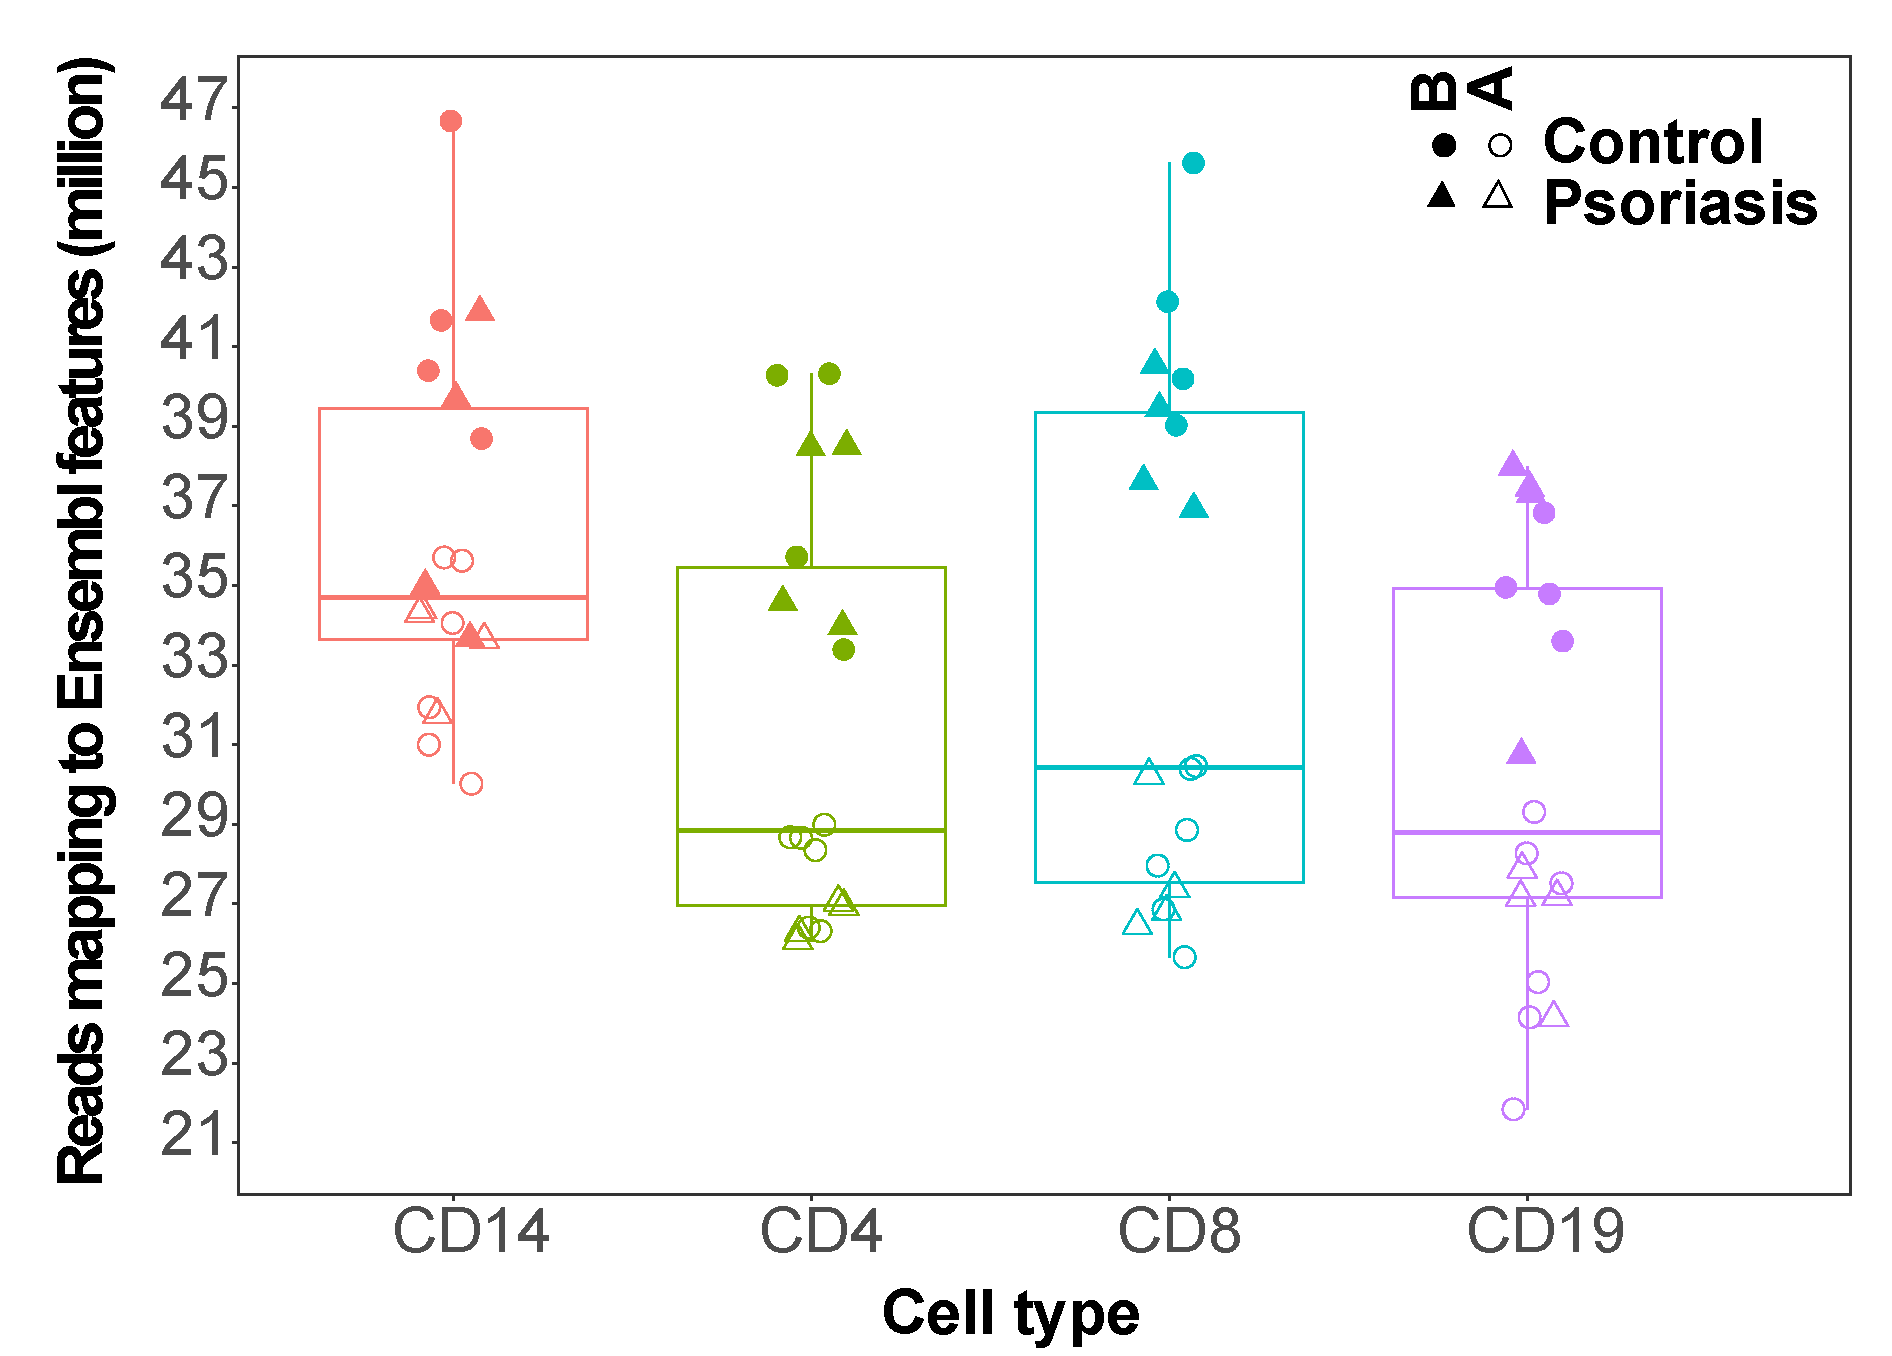
\includegraphics[width=\textwidth]{./Appendix/pdfs/Chapter4/PS_CTL_RNAseq_total_reads_per_batch_cell_type_and_condition}
\caption{\textbf{}}
\end{subfigure}
\caption[Mapping rate and total reads after filtering (million) mapping to Ensembl genes in all the RNA-seq samples from psoriasis patients and controls in four cell types.]{\textbf{Mapping rate and total reads after filtering (million) mapping to Ensembl genes in all the RNA-seq samples from psoriasis patients and controls in four cell types.} (A) The mapping rate refers to the percentage of total sequenced reads from each sample that uniquely mapped to a particular site of the genome. (B) The total number of reads after filtering for non-uniquely mapped and duplicated reads that mapped to Ensembl features, including coding protein genes and lncRNAs.}
\label{figure:RNAseq_mapping_rate_and_reads_in_genes}
\end{figure} 


\begin{figure}[htbp]
\centering
\begin{subfigure}{0.45\textwidth}
\centering
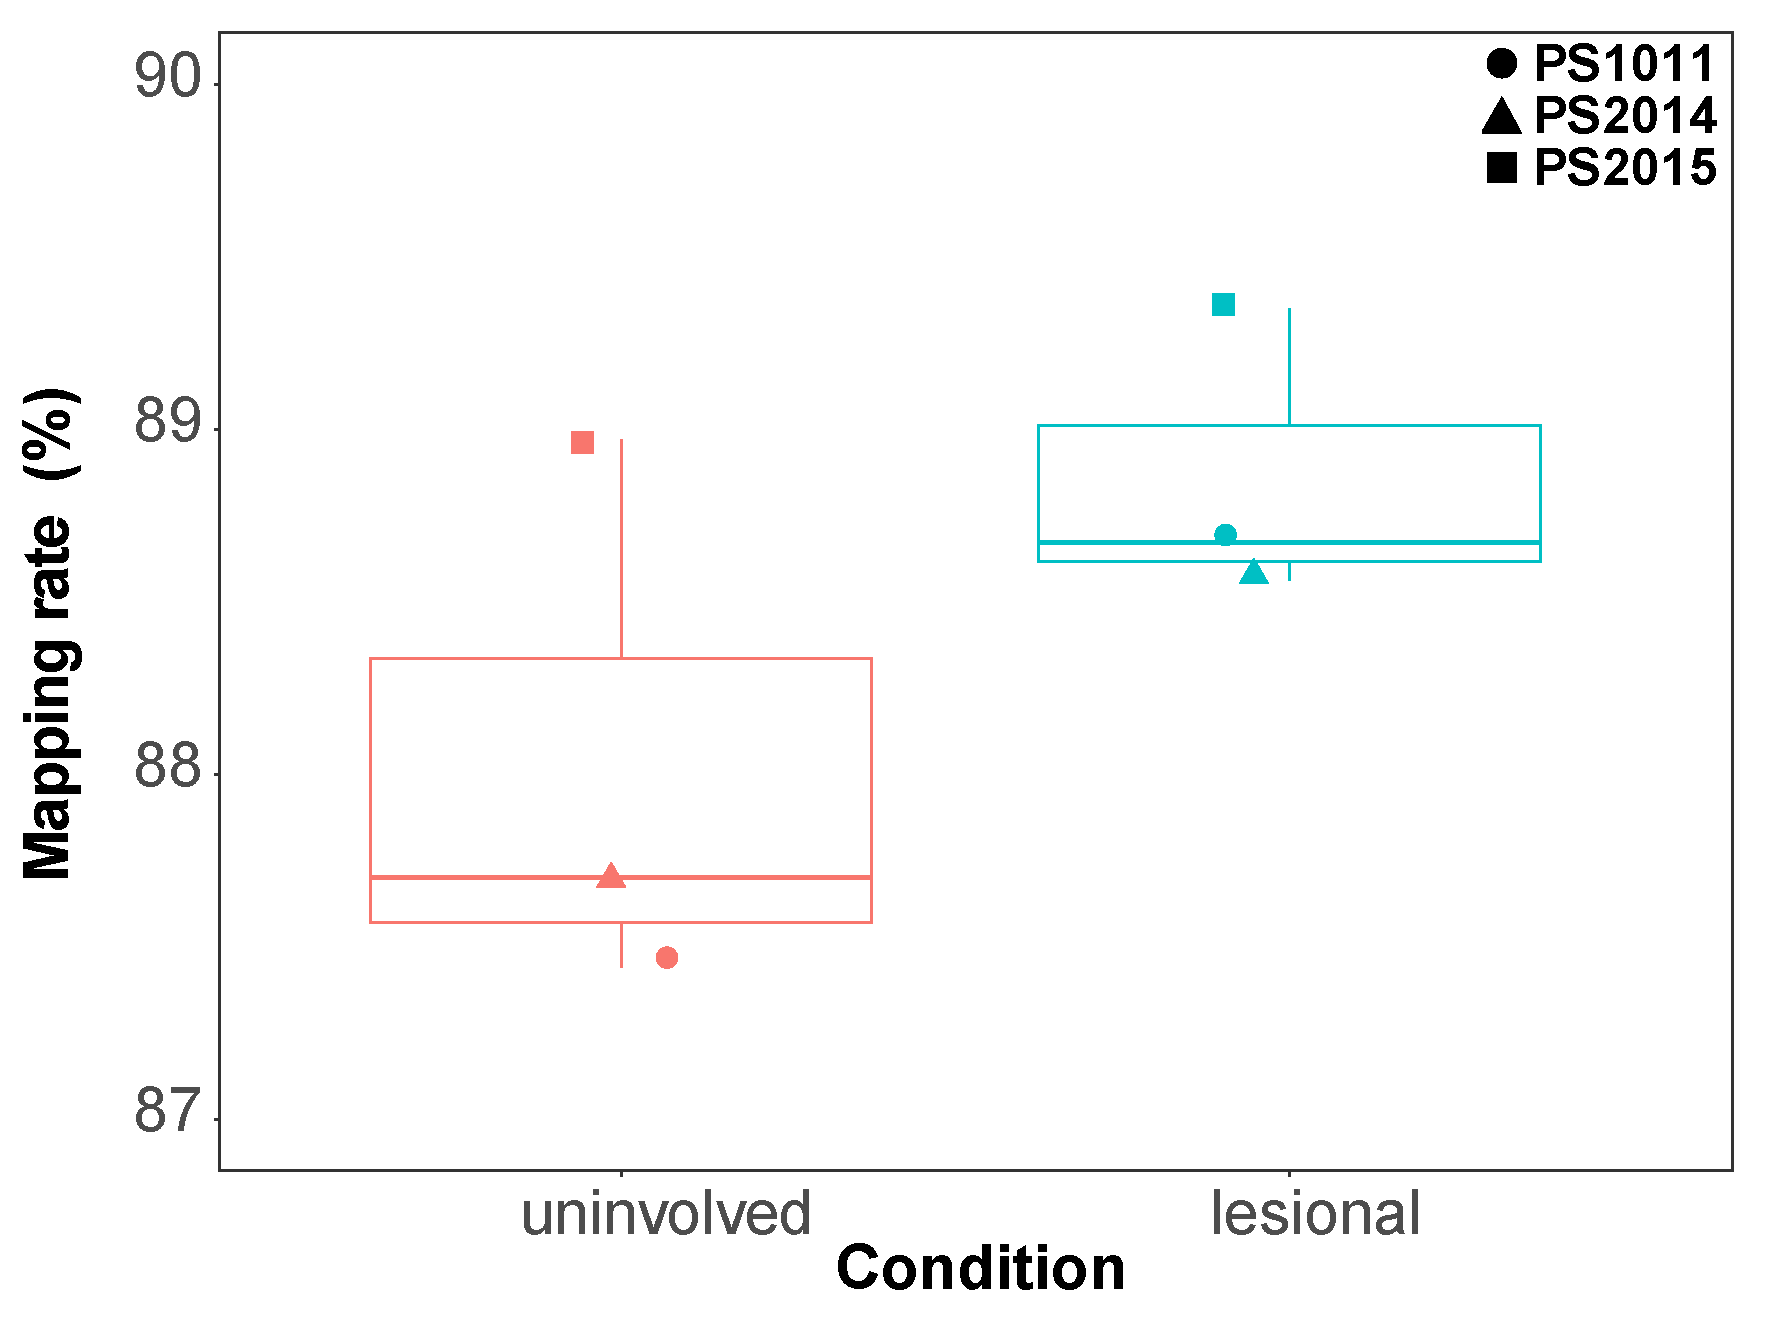
\includegraphics[width=\textwidth]{./Appendix/pdfs/Chapter4/PS_lesional_uninvolved_RNAseq_uniquely_mapped_reads_percent_cell_type_and_batch_boxplots}
\caption{\textbf{}}
% The percentage sign indicated that the other subfig goes side by side
\end{subfigure}%
\begin{subfigure}{0.45\textwidth}
\centering
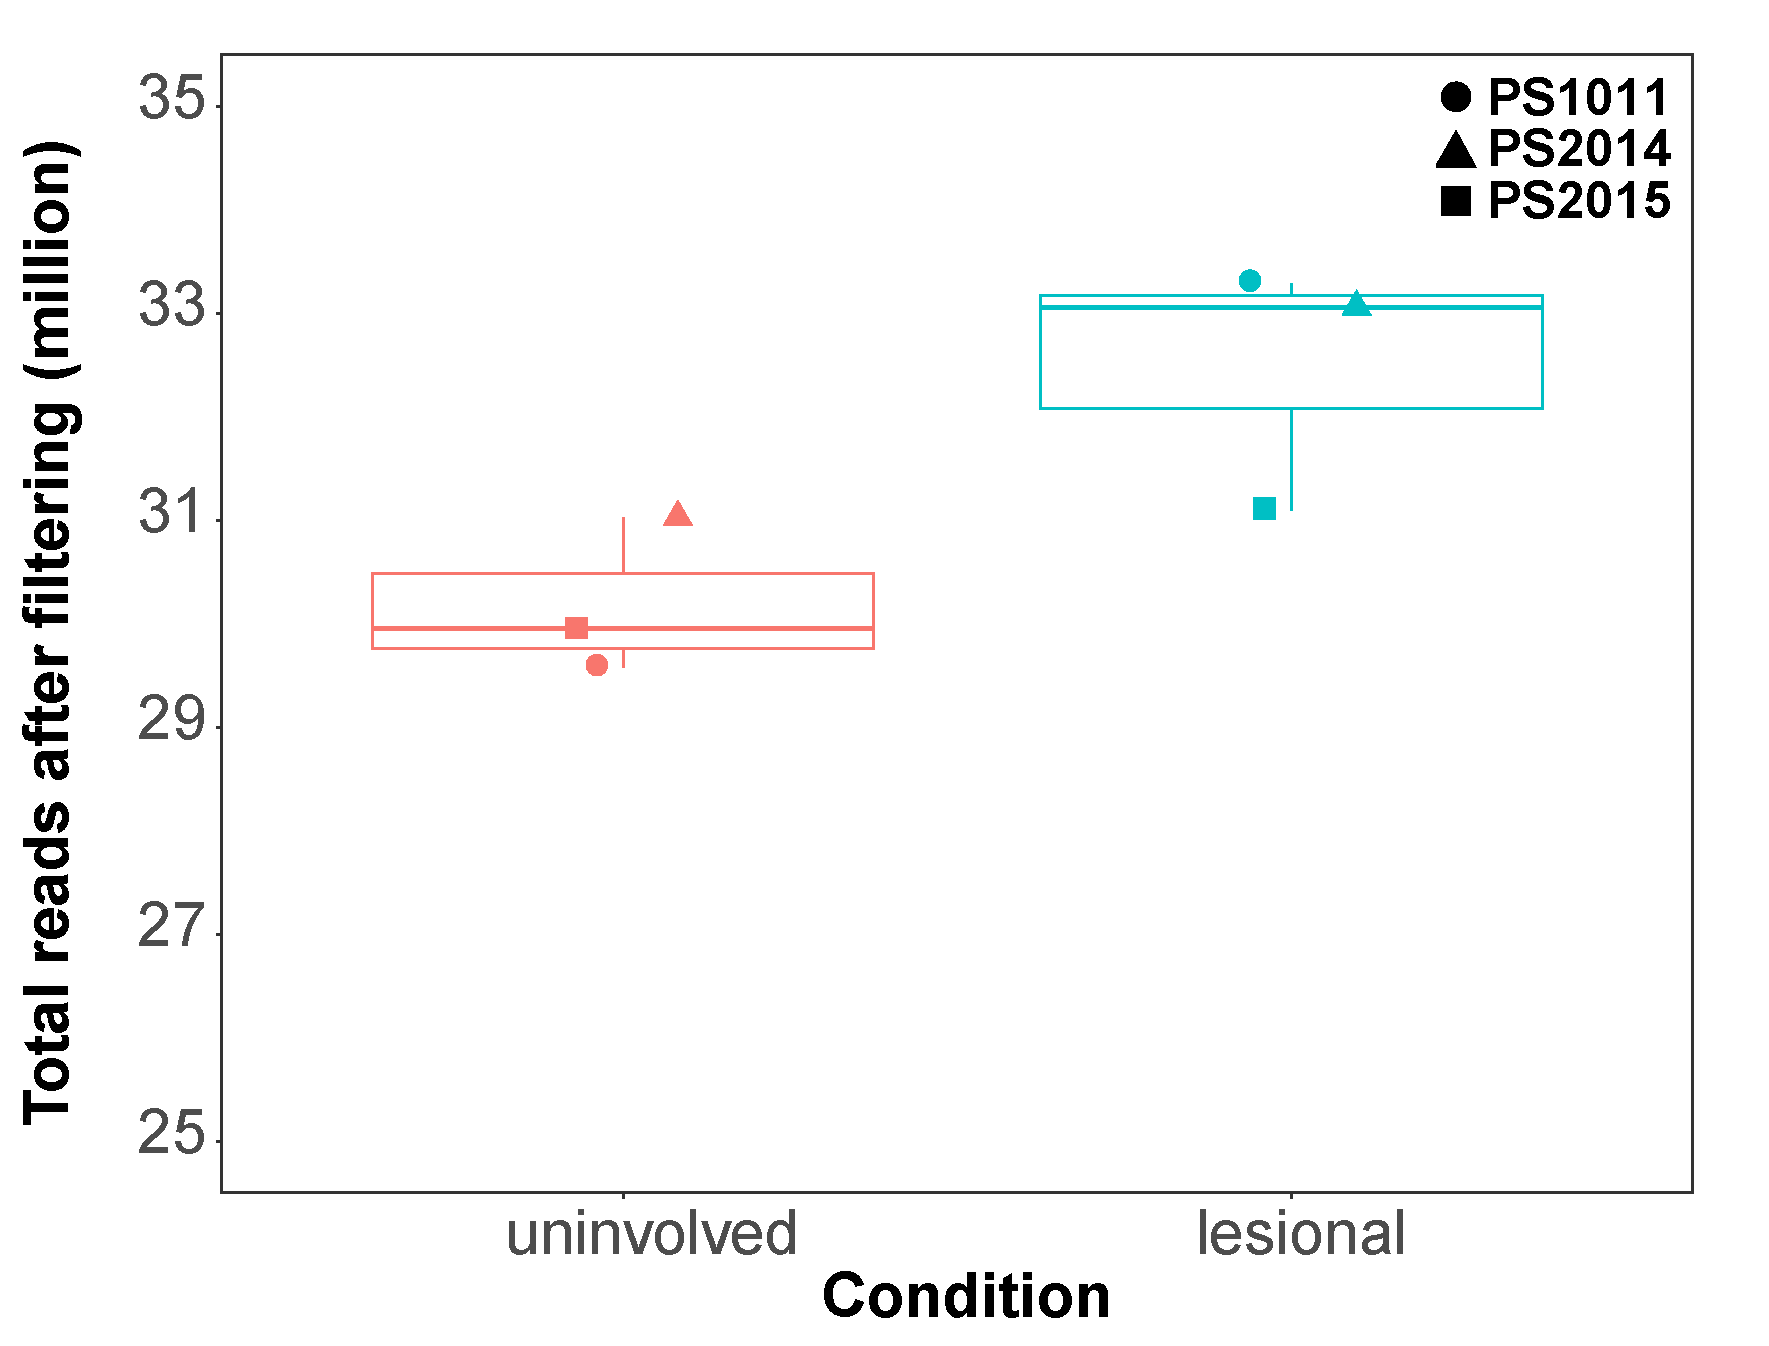
\includegraphics[width=\textwidth]{./Appendix/pdfs/Chapter4/PS_lesional_uninvolved_RNAseq_total_reads_per_cell_type_and_batch}
\caption{\textbf{}}
\end{subfigure} \\
\caption[Mapping quality control for the RNA-seq data in the uninvolved and lesional epidermis from psoriasis patients.]{\textbf{Mapping quality control for the RNA-seq data in the uninvolved and lesional epidermis from psoriasis patients.} (A) Mapping rate calculated as the proportion of sequencing reads mapping uniquely to a particular region of the genome. (B) The total number of reads mapping to an Ensembl feature (including protein coding genes and lncRNAs) after removing the non-uniquely mapped and duplicated reads. }
\label{figure:RNAseq_PS_uninvolved_lesional_psoriasis_skin_mapping}
\end{figure}


\begin{figure}[htbp]
	\centering
	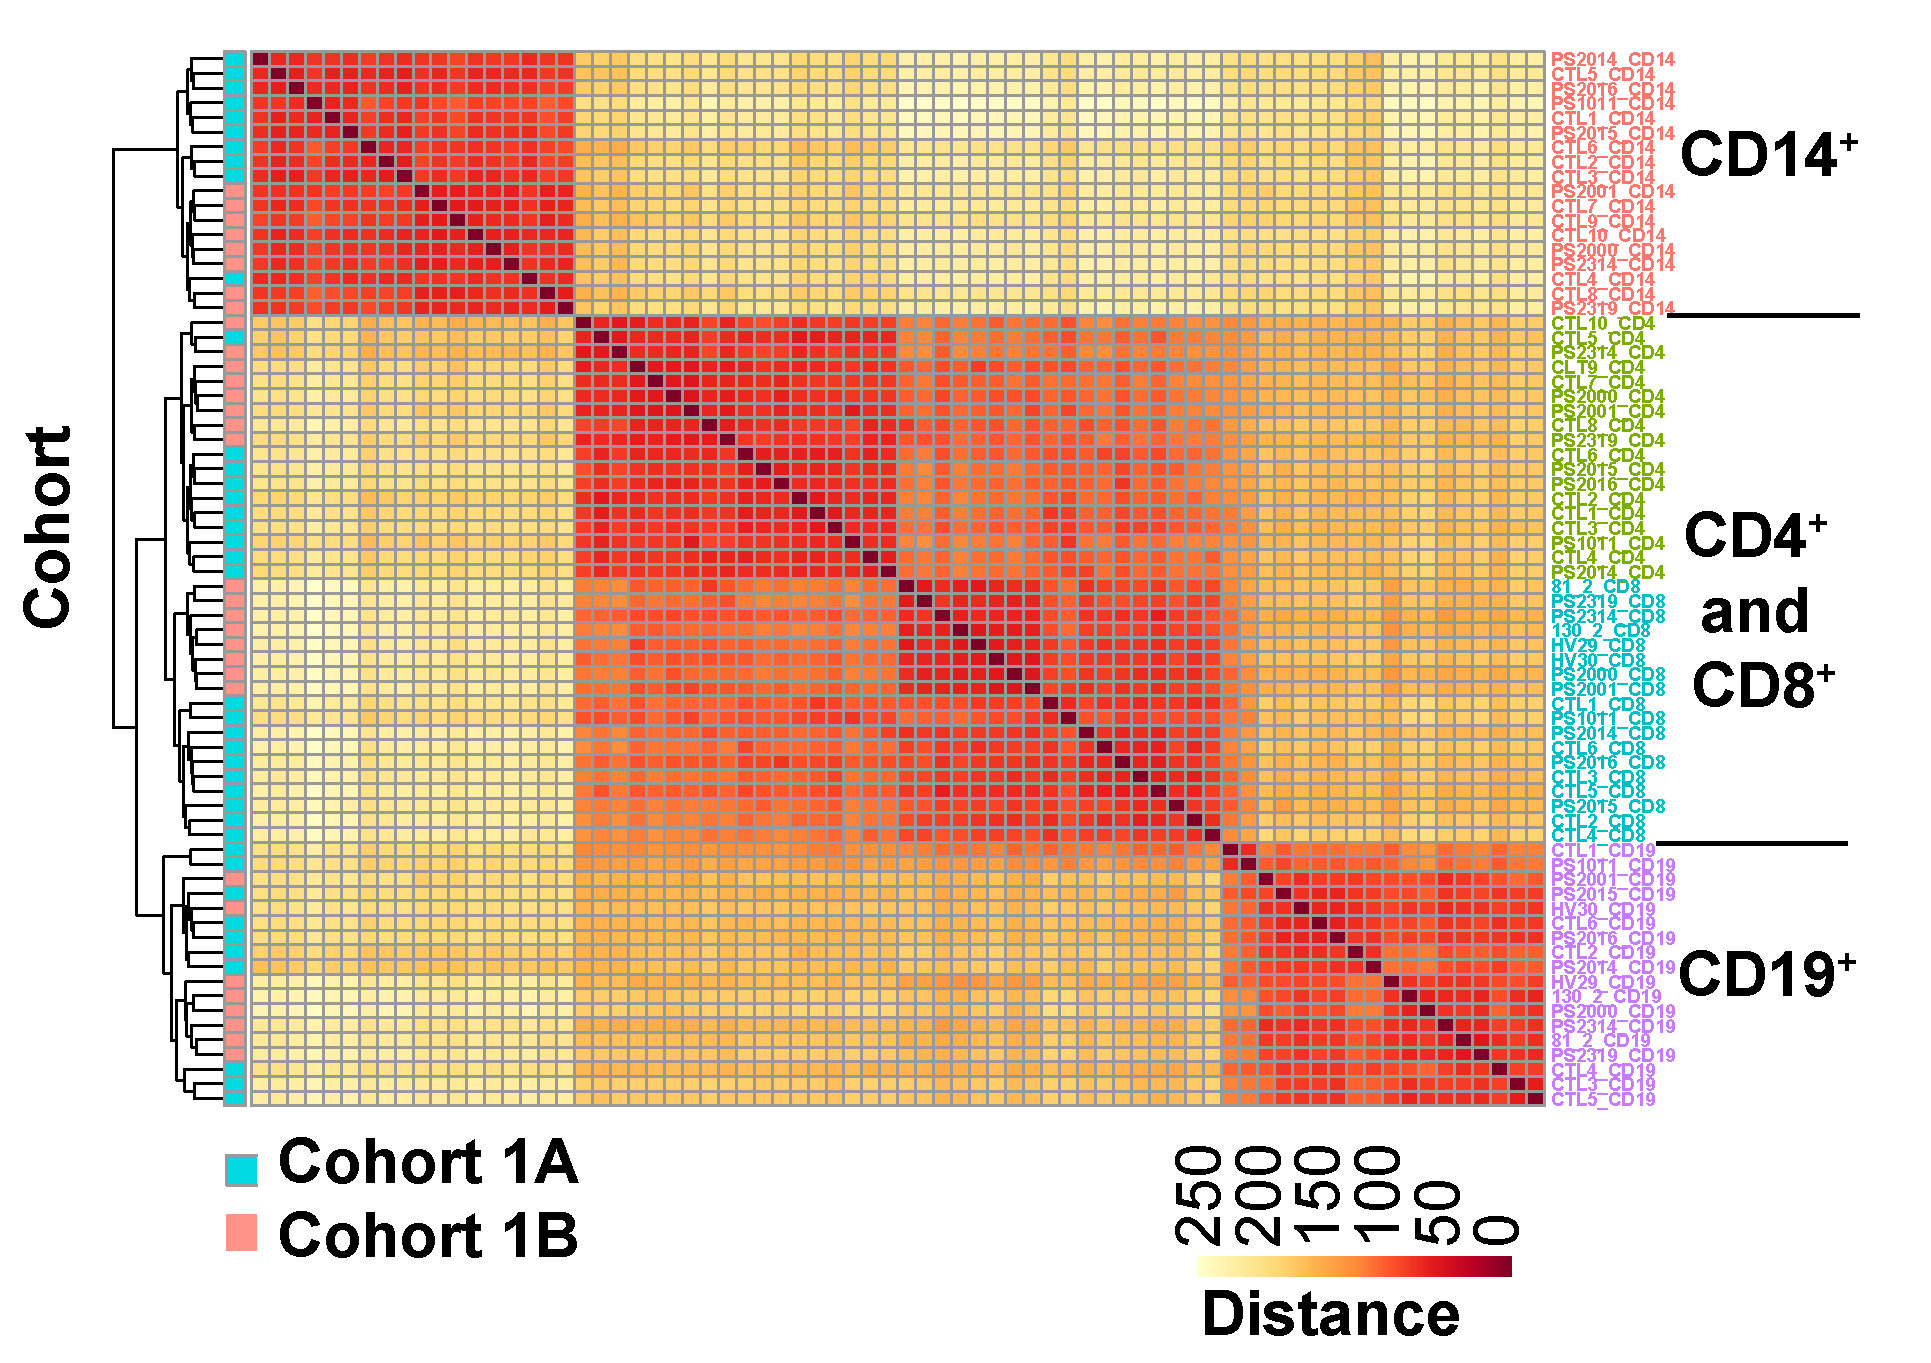
\includegraphics[width=0.6\textwidth]{./Results2/pdfs/PS_CTL_all_samples_heatmap_including_batch}
\caption[Distance heatmap with hierarchical clustering illustrating the sample variability based on the gene expression profiles for all 72 samples.]{\textbf{Distance heatmap with hierarchical clustering illustrating the sample variability based on the gene expression profiles for all 72 samples.} Distance matrix built based on normalised read counts mapping to 20,493 Ensembl featured remaining after appropriate filtering followed by hierarchical clustering of the samples. Additional annotation of the clustering based on cohort identity is included on the left hand side.}
\label{figure:RNAseq_heat_map}
\end{figure}
\


\begin{figure}[htbp]
\centering
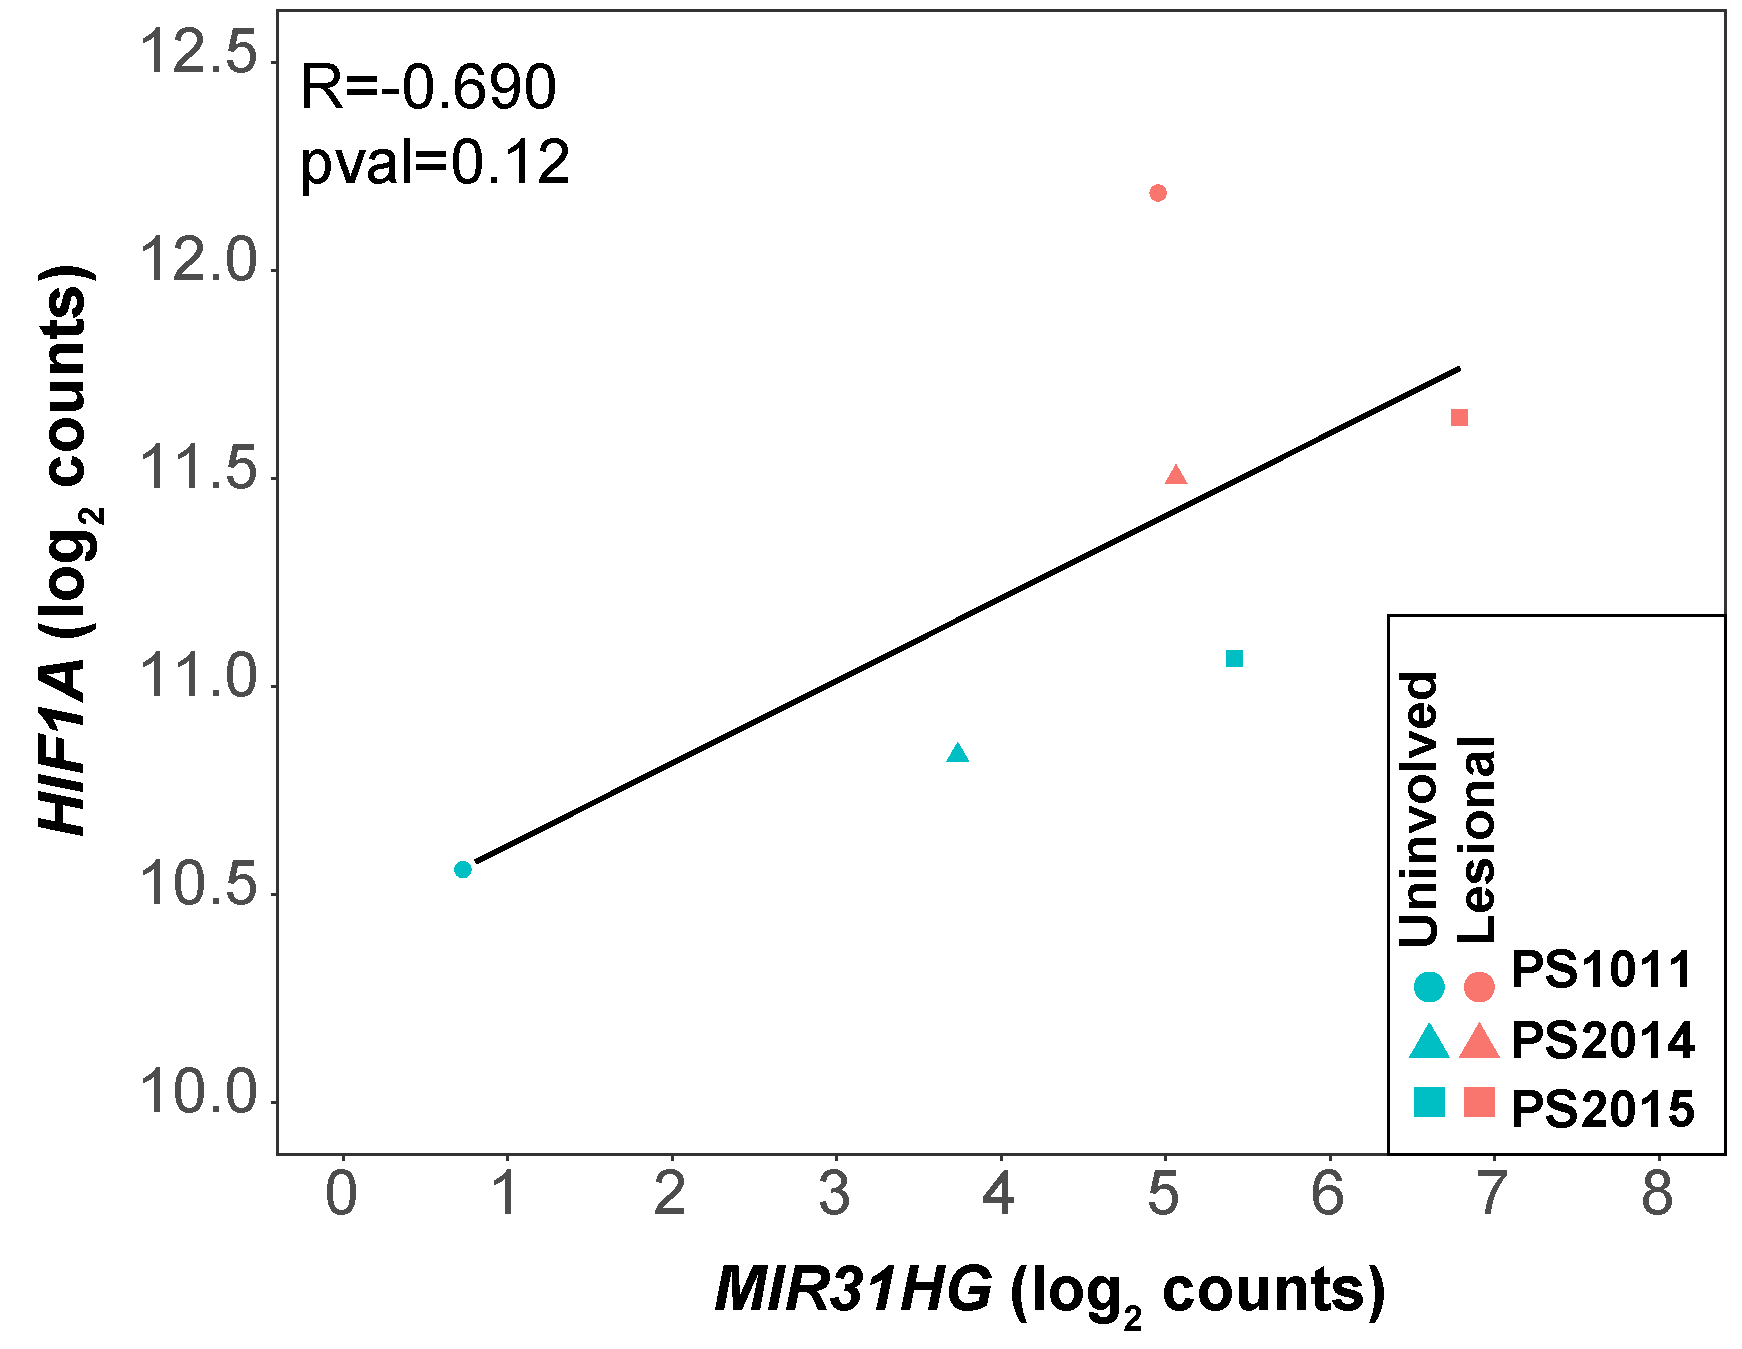
\includegraphics[width=0.45\textwidth]{./Appendix/pdfs/Chapter4/Skin_RNAseq_correlation_MIR31HG_HIF1A_plot}
\caption[Correlation in gene expression between the miRs \textit{MIR31HG} and the target gene \textit{HIF-1A} in lesional and uninvolved skin.]{\textbf{Correlation in gene expression between the miRs \textit{MIR31HG} and the target gene \textit{HIF-1A} in lesional and uninvolved skin.} Plot showing the correlation in log$_2$ normalised read counts for \textit{MIR31HG} and \textit{HIF-1A}. Pearson correlation values (R) and significance (p-value) are included. Each of the dots represents one samples, where colour represents condition (lesional or uninvolved) and shape corresponds to the patient ID.}
\label{figure:RNAseq_lesional_uninvolved_miR_correlations}
\end{figure}


\begin{figure}[htbp]
\centering
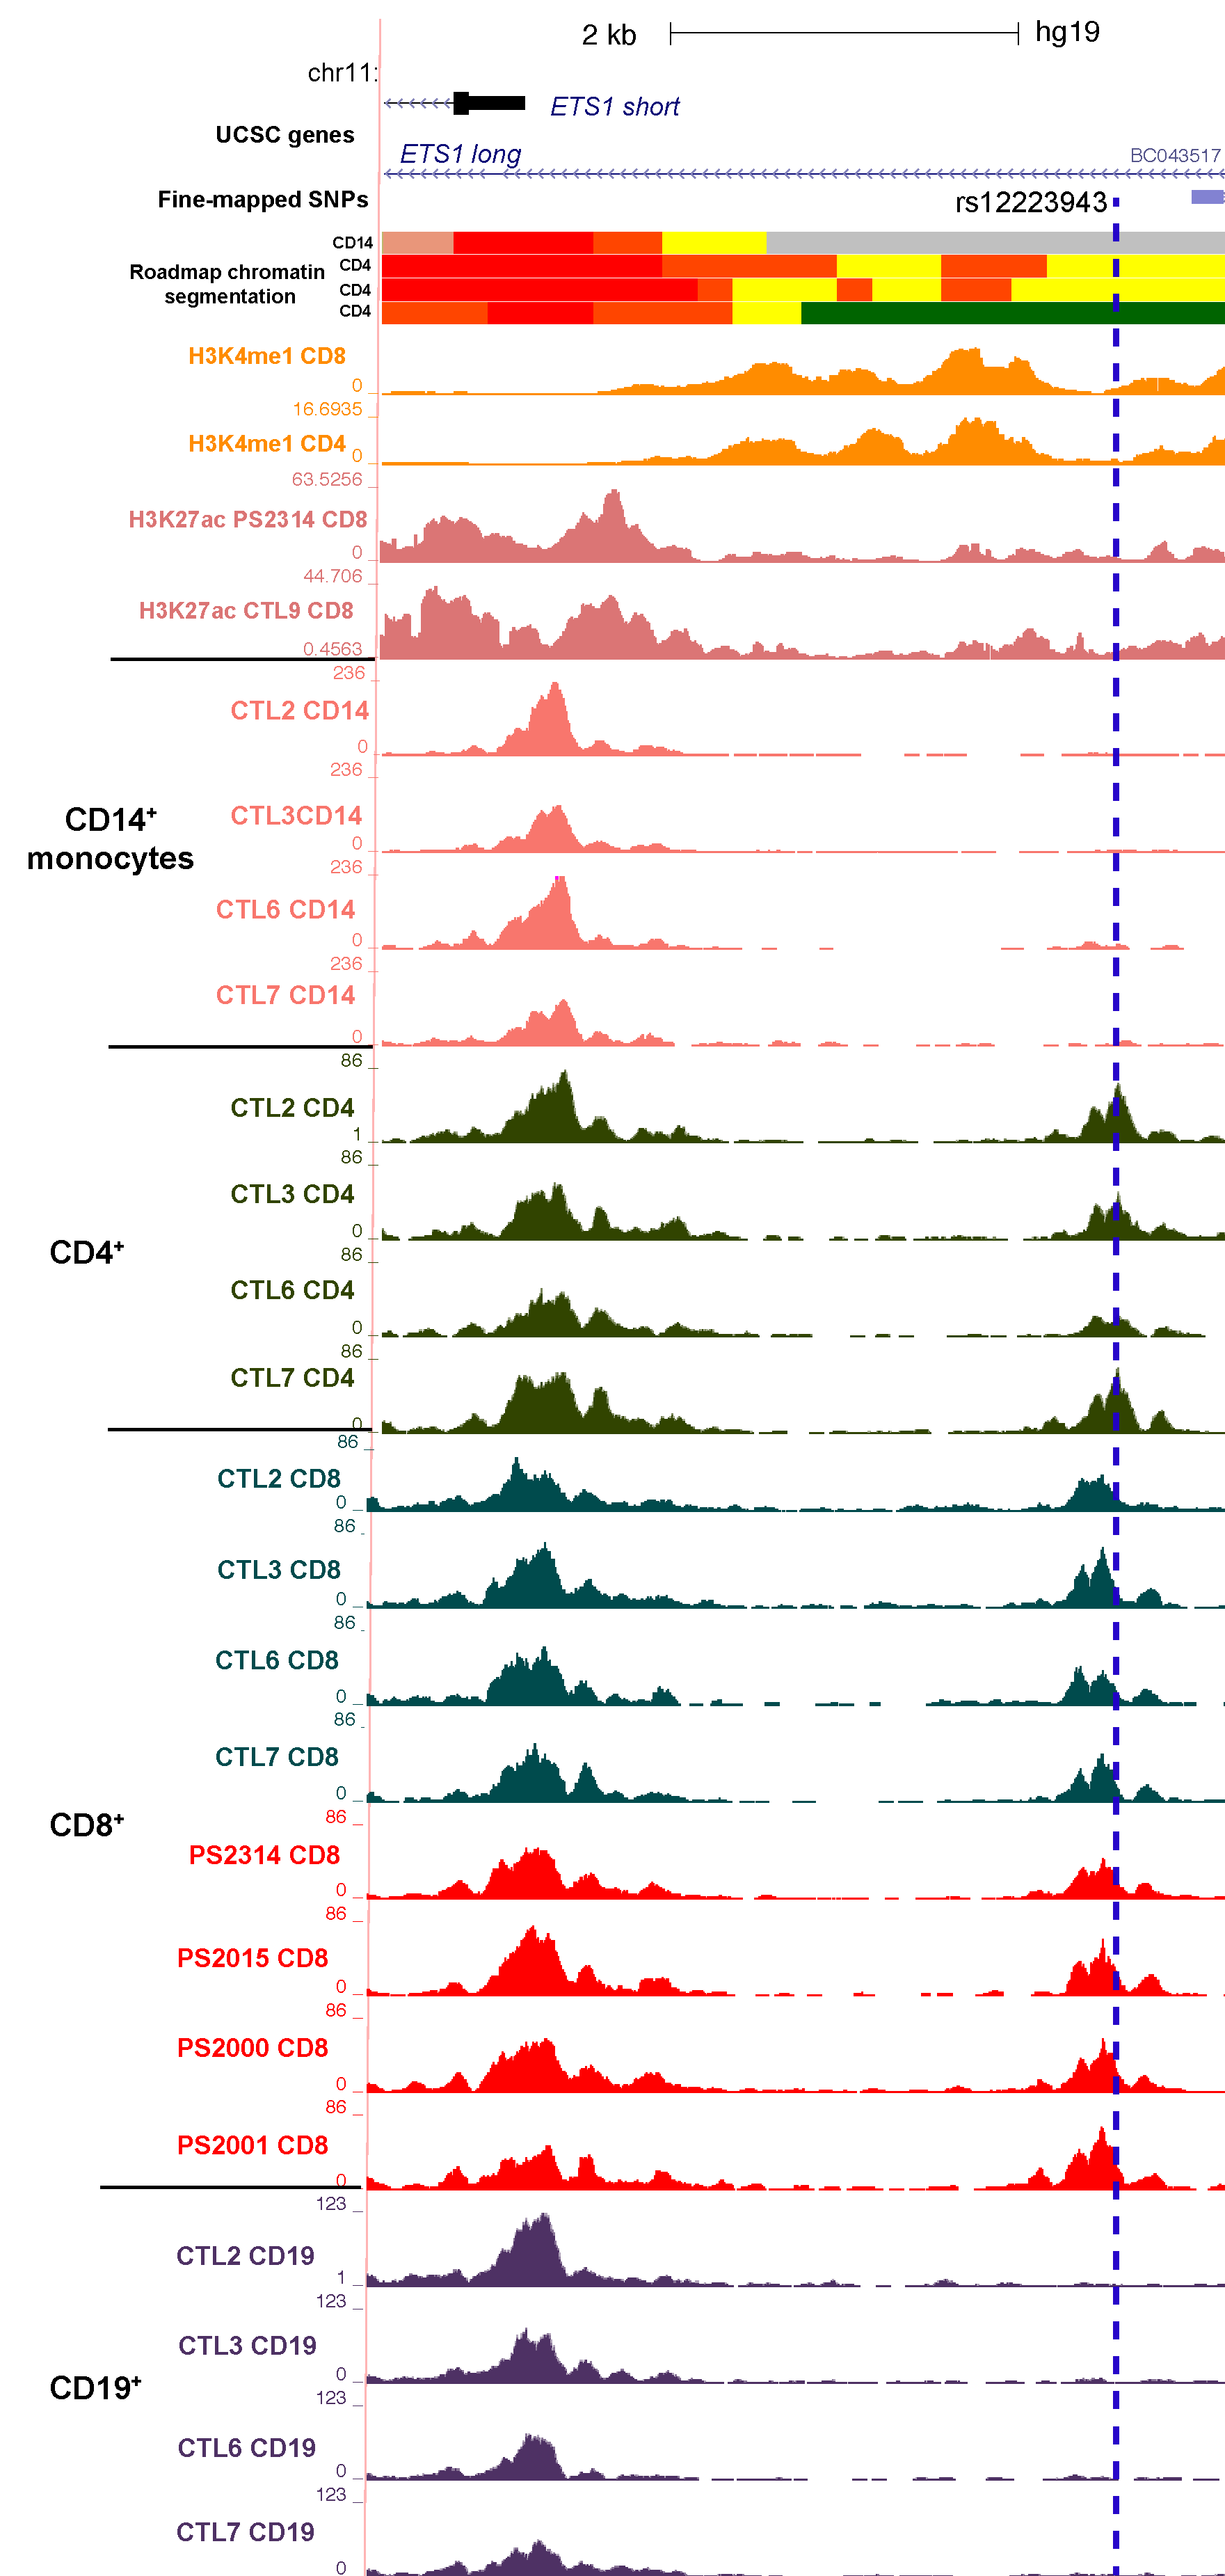
\includegraphics[width=0.55\textwidth]{./Appendix/pdfs/Chapter4/UCSC_ETS1_credible_set_track}
\caption[Epigenetic landscape at the location of the fine-mapped SNP rs12223943 at the \textit{ETS1} psoriasis GWAS locus.]{\textbf{Epigenetic landscape at the location of the fine-mapped SNP rs12223943 at the \textit{ETS1} psoriasis GWAS locus.} UCSC Genome Browser view illustrating normalised ATAC read density and H3K27ac fold-enrichment as well as publicly available epigenetic datasets (chromatin segmentation map and H3K4me1) (y-axis) at the location (x-axis) of the fine-mapped SNP rs12223943 (blue dashed line). Only representative ATAC tracks from control samples are shown for CD14$^+$ monocytes, CD4$^+$ and CD19$^+$ cells.}
\label{figure:ATAC_PS_CTL_ETS1_FM}
\end{figure}




\clearpage

\section{Chapter 5 Figures}


\bigskip
\begin{figure}[H]
\centering
\begin{subfigure}[b]{0.48\textwidth}
\centering 
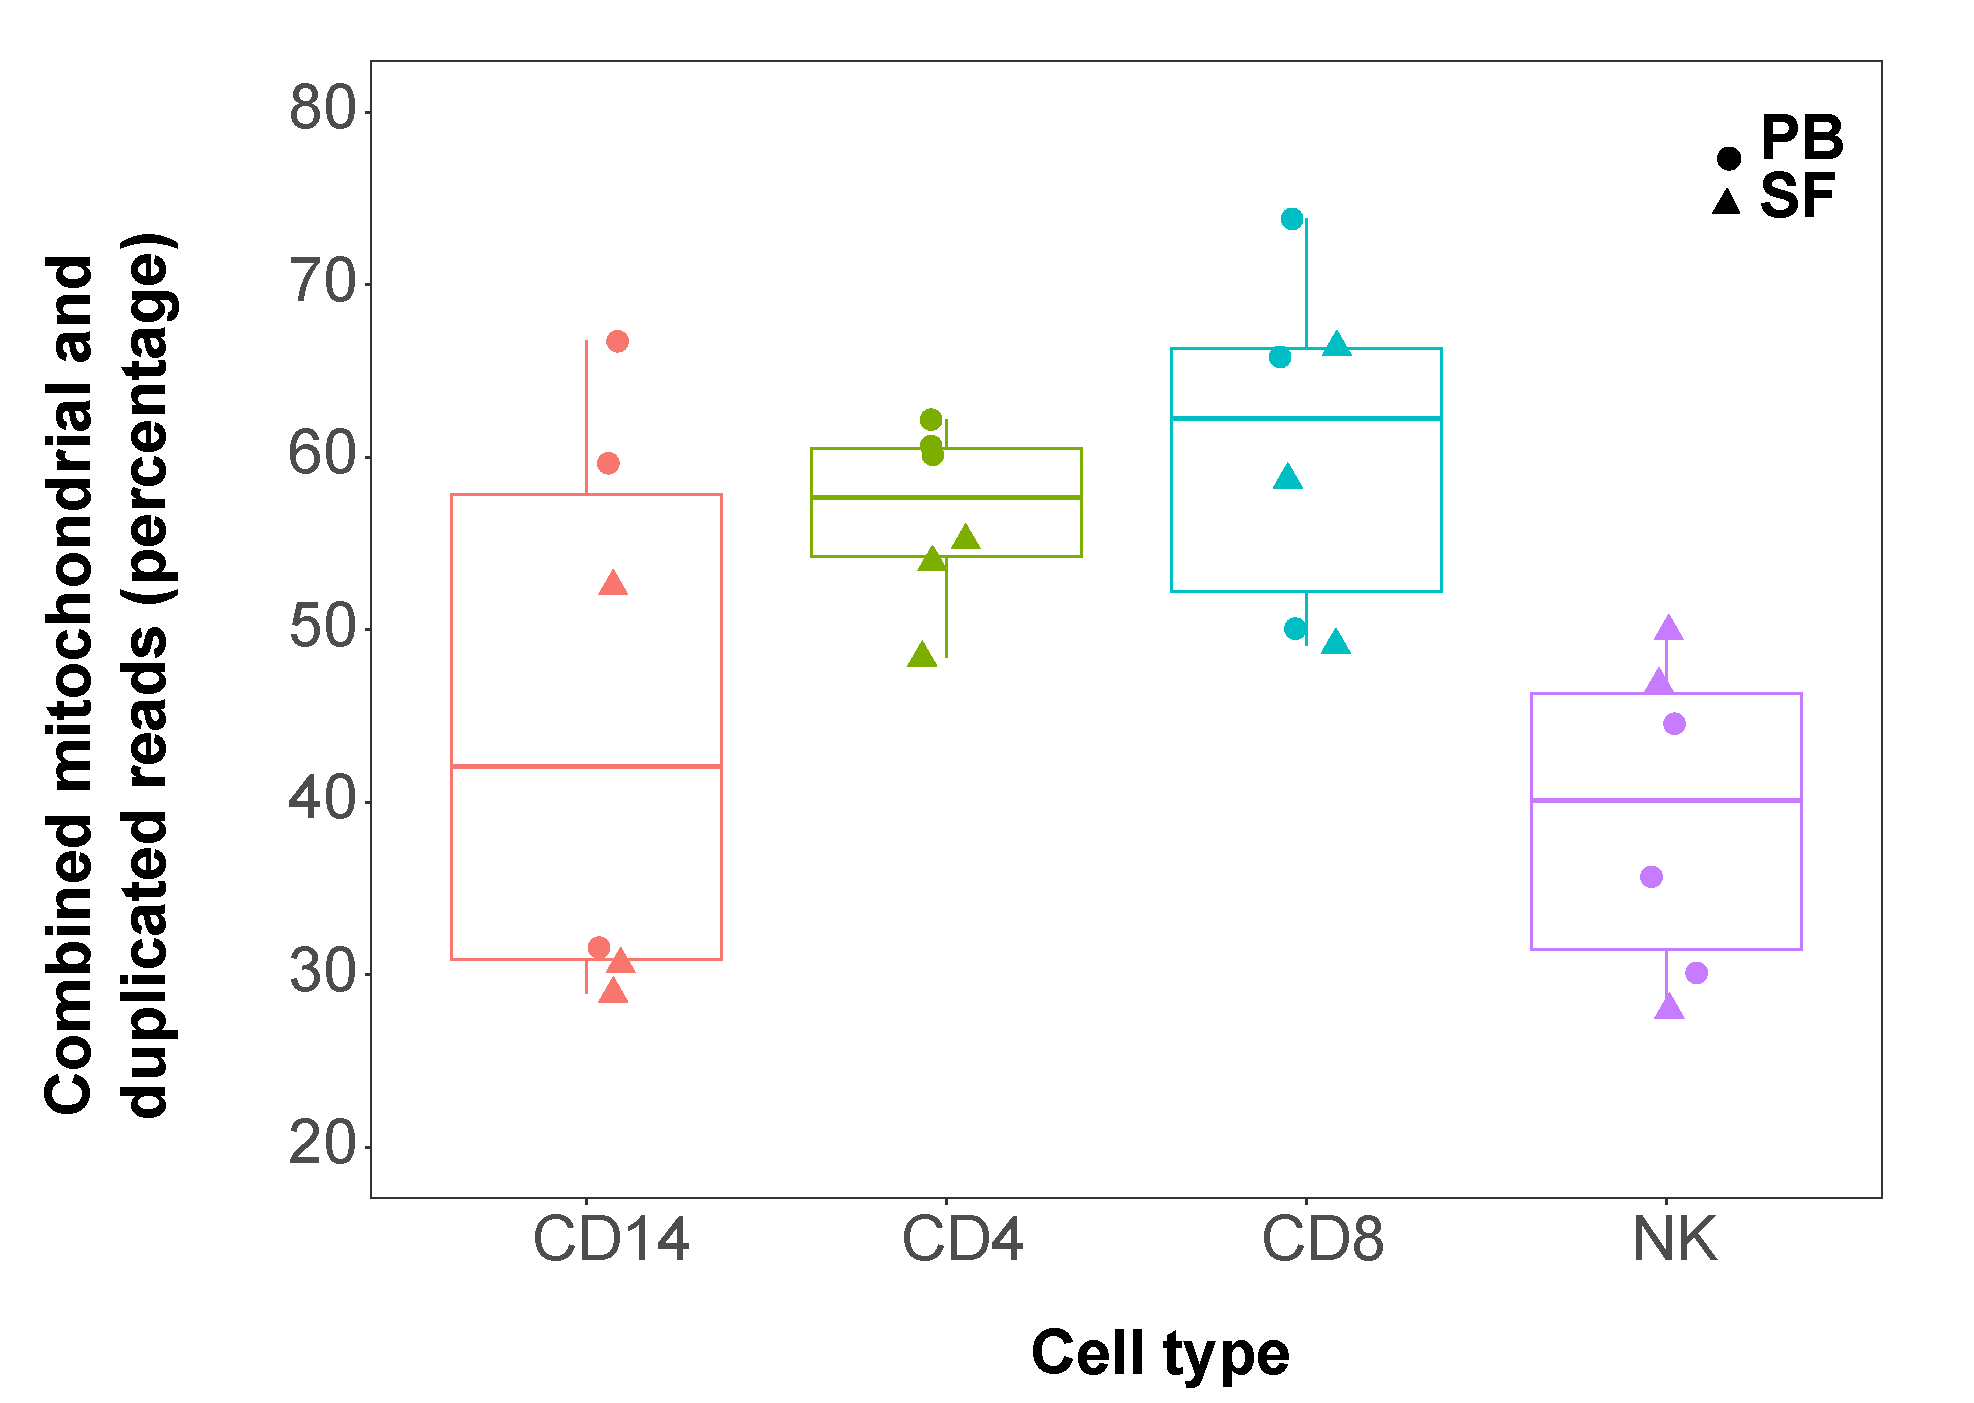
\includegraphics[width=\textwidth]{./Appendix/pdfs/Chapter5/ATAC_PSA_pcnt_dups_and_MT_reads_boxplot}
\caption{}
\end{subfigure}%
~
\begin{subfigure}[b]{0.48\textwidth} 
%the [b] prevents offset in subcaptions
\centering
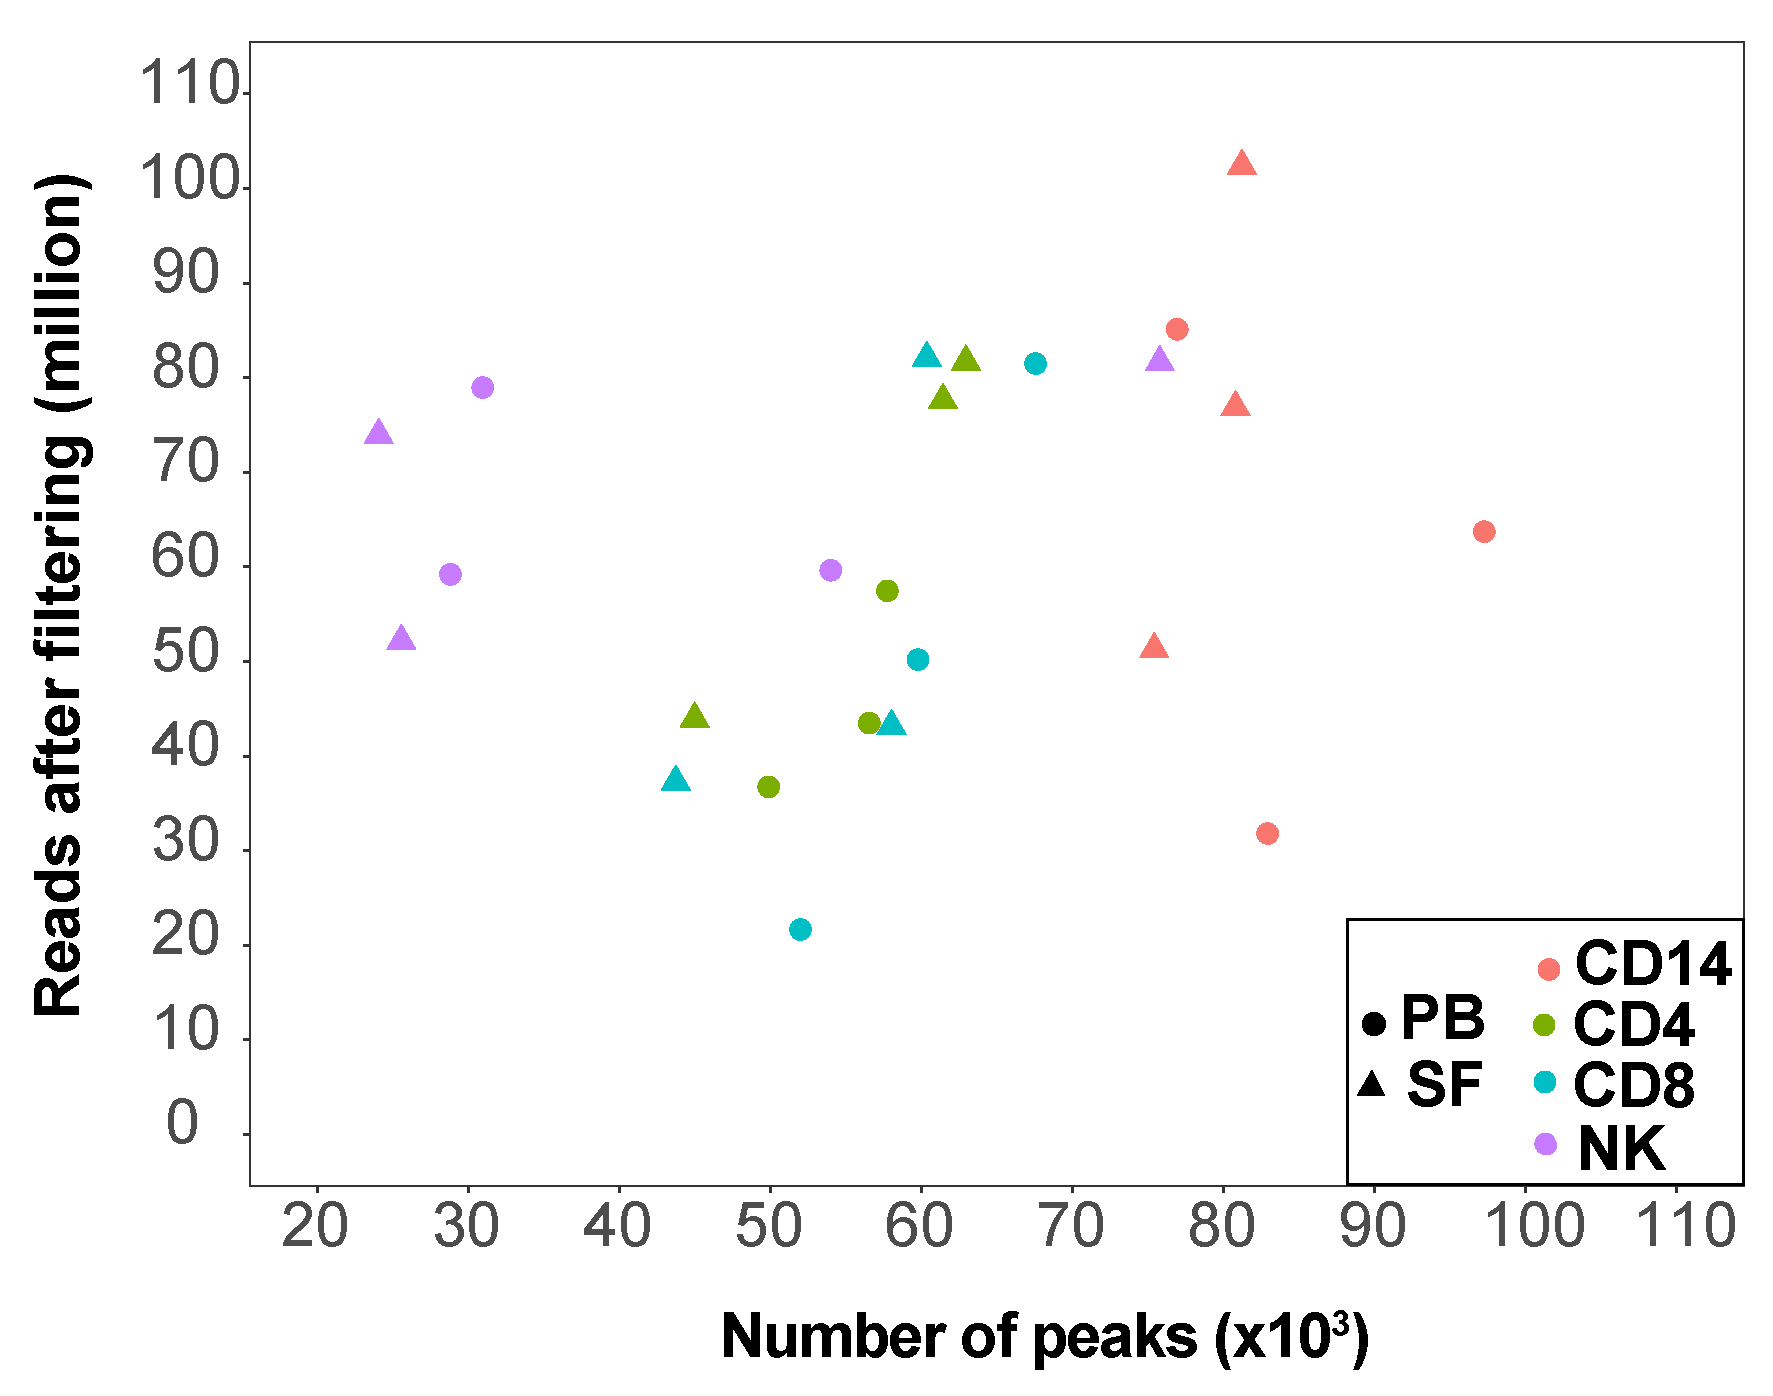
\includegraphics[width=\textwidth]{./Appendix/pdfs/Chapter5/ATAC_PSA_all_peaks_vs_num_reads}%
\caption{}
\end{subfigure}
\caption[Assessment of the percentage of mitochrondrial and duplicated reads and the number of called peaks after filtering in the ATAC data from peripheral blood and synovial fluid of PsA patients samples.]{\textbf{Assessment of the percentage of  mitochrondrial and duplicated reads and the number of called peaks after filtering in the ATAC data from peripheral blood and synovial fluid of PsA patients samples.} For each of the cell types and samples (A) boxplot representing percentage of duplicated and mitochondrial reads combined and (B) representation of the  number of significant peaks after filtering based on IDR optimal p-values versus the total million reads after filtering for each of the samples. For each point, colour codes for cell type and shape for tissue (SF=synovial fluid; PB=peripheral blood).}
\label{figure:PsA_FAST_ATAC_QC_supplementary}
\end{figure}


%\begin{figure}[htbp]
%\centering
%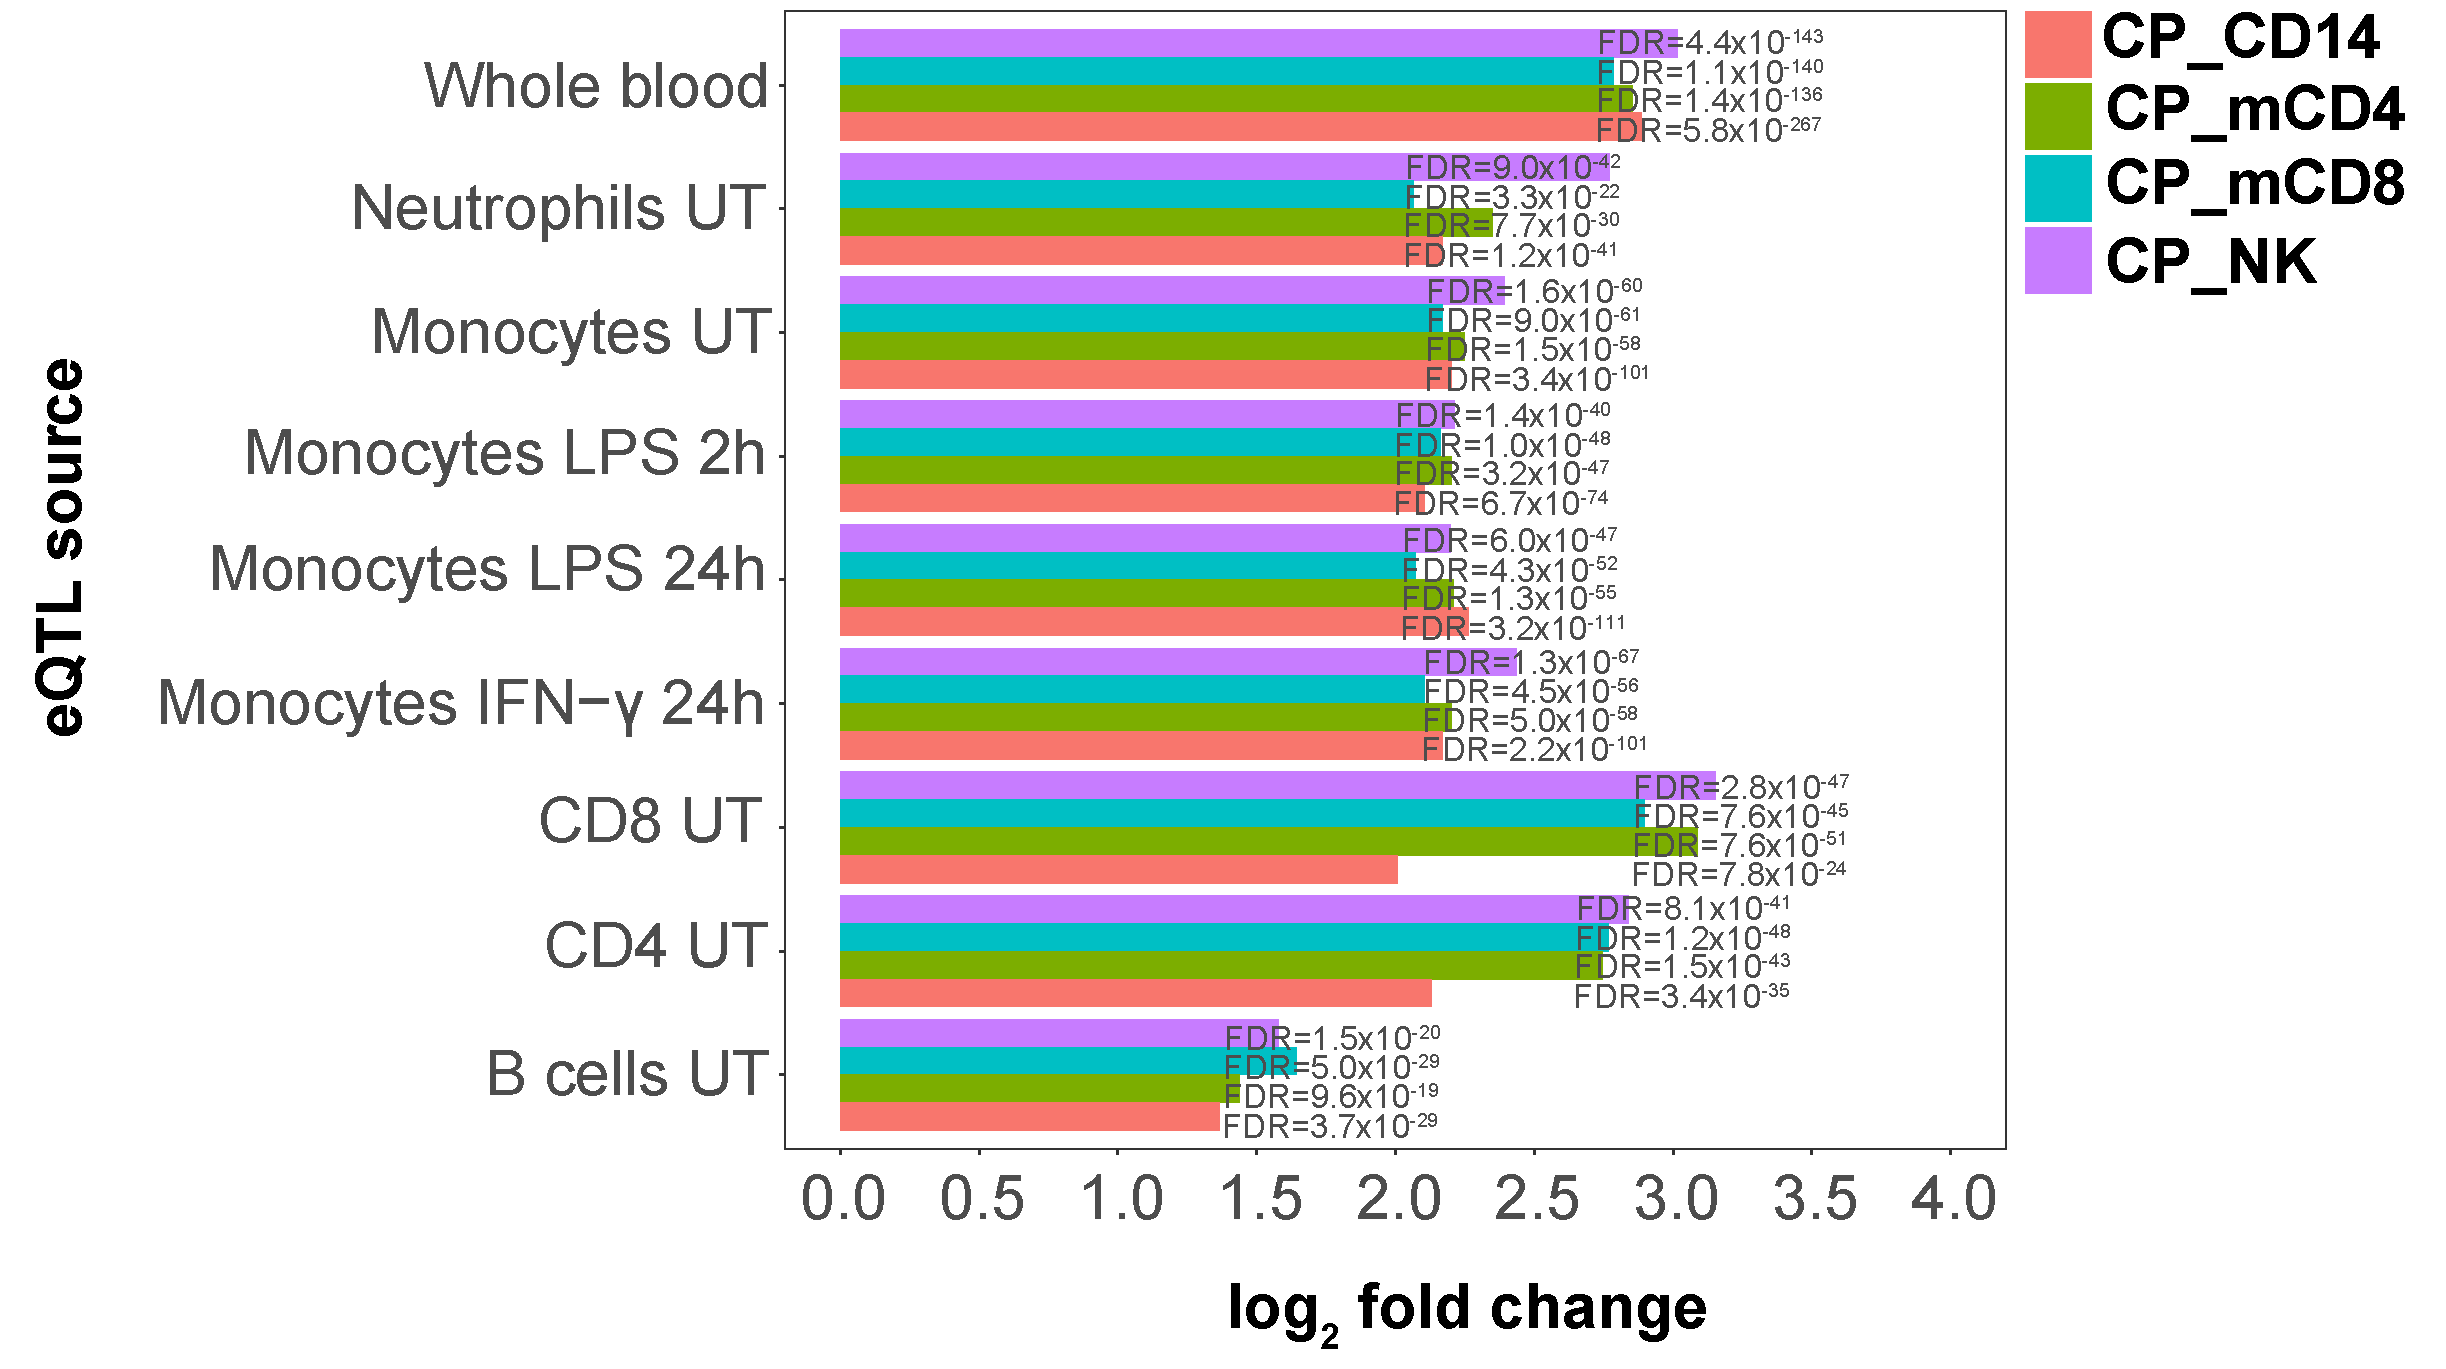
\includegraphics[width=0.6\textwidth]{./Appendix/pdfs/Chapter5/PSA_ATAC_consensus_list_eQTL_enrichment_all_cell_types}
%\caption[Enrichment of eQTL SNPs for the consensus list of ATAC peaks used to perform differential chromatin accessibility analysis in each cell type.]{\textbf{Enrichment of eQTL SNPs for the consensus list of ATAC peaks used to perform differential chromatin accessibility analysis in each cell type.} Barplot illustrating for the consensus list of ATAC peaks in of the 4 assayed cell types the log2 fold change and significance (FDR) of the top enriched GTEx eQTL dataset (whole blood) and the publicly available eQTL datasets in immune cell types. Although enrichment of eQTL SNPs in the majority of GTEx datasets for the consensus list of peaks in the 4 cell types was found, whole blood presented the largest and most significant enrichment amongst all of them}
%\label{figure:eQTL_enrichment_CP_all_cell_types}
%\end{figure}


\begin{figure}[htbp]
\centering
\begin{subfigure}[b]{0.45\textwidth}
\centering 
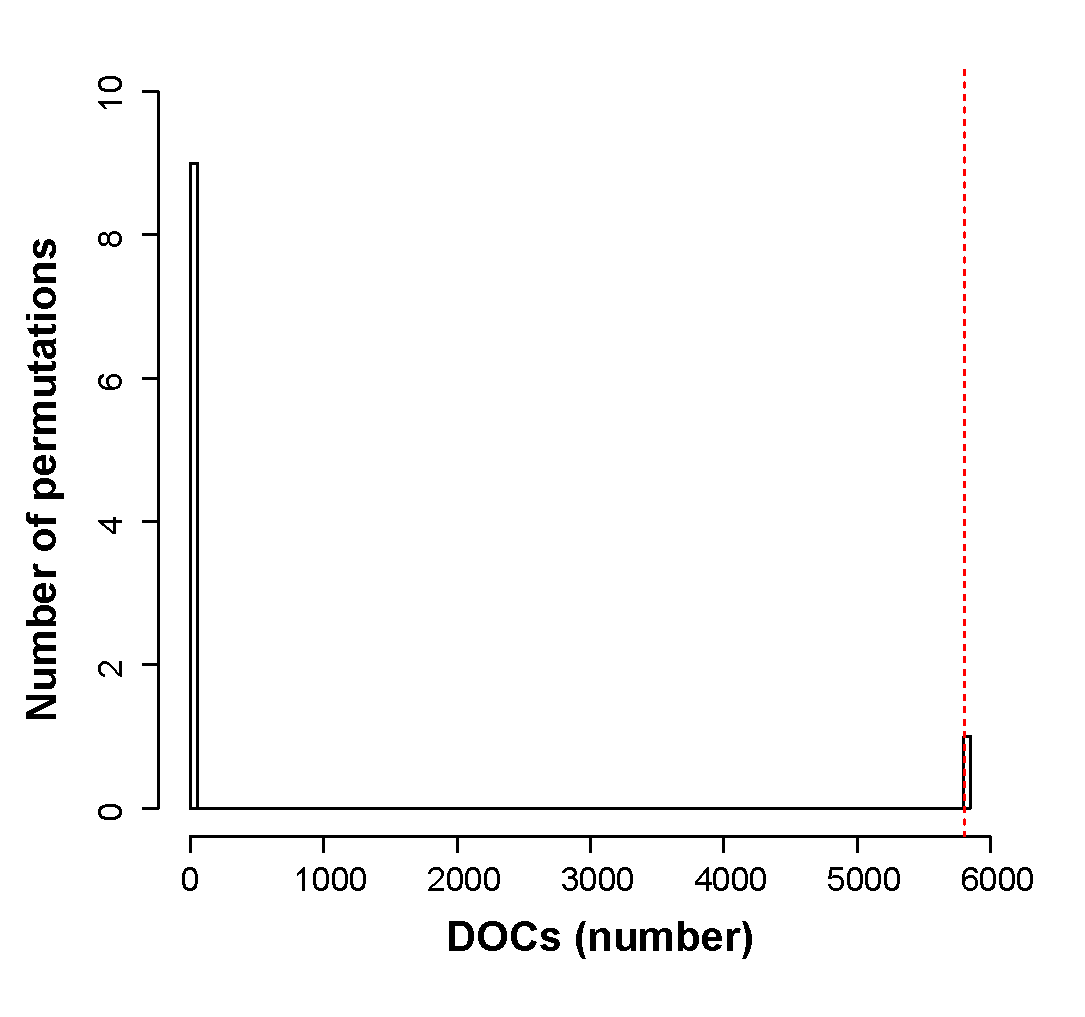
\includegraphics[width=\textwidth]{./Appendix/pdfs/Chapter5/ATAC_PsA_CD14_permutation_analysis}
\caption{}
\end{subfigure}
~
\begin{subfigure}[b]{0.45\textwidth}
\centering 
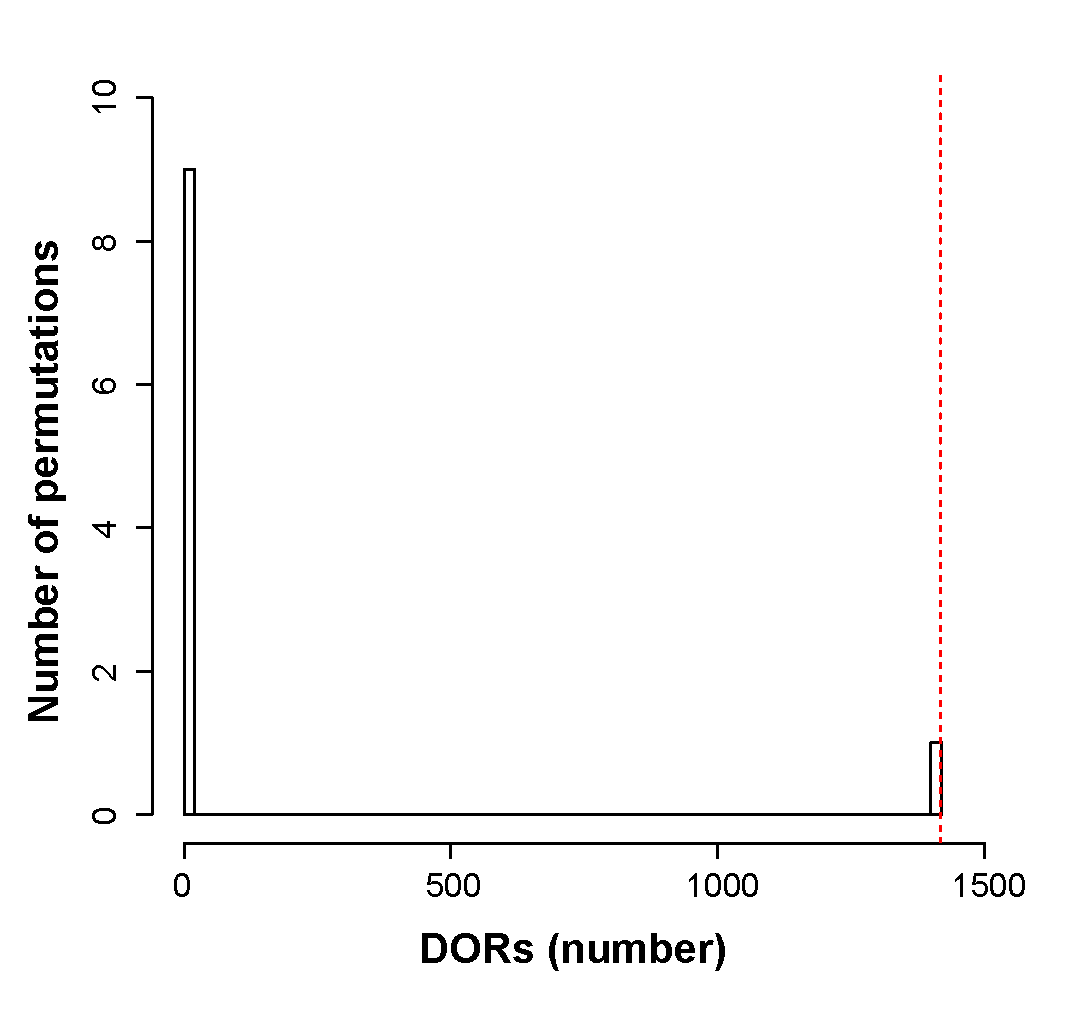
\includegraphics[width=\textwidth]{./Appendix/pdfs/Chapter5/ATAC_PsA_CD4_permutation_analysis}
\caption{}
\end{subfigure}
~
\begin{subfigure}[b]{0.45\textwidth} 
%the [b] prevents offset in subcaptions
\centering
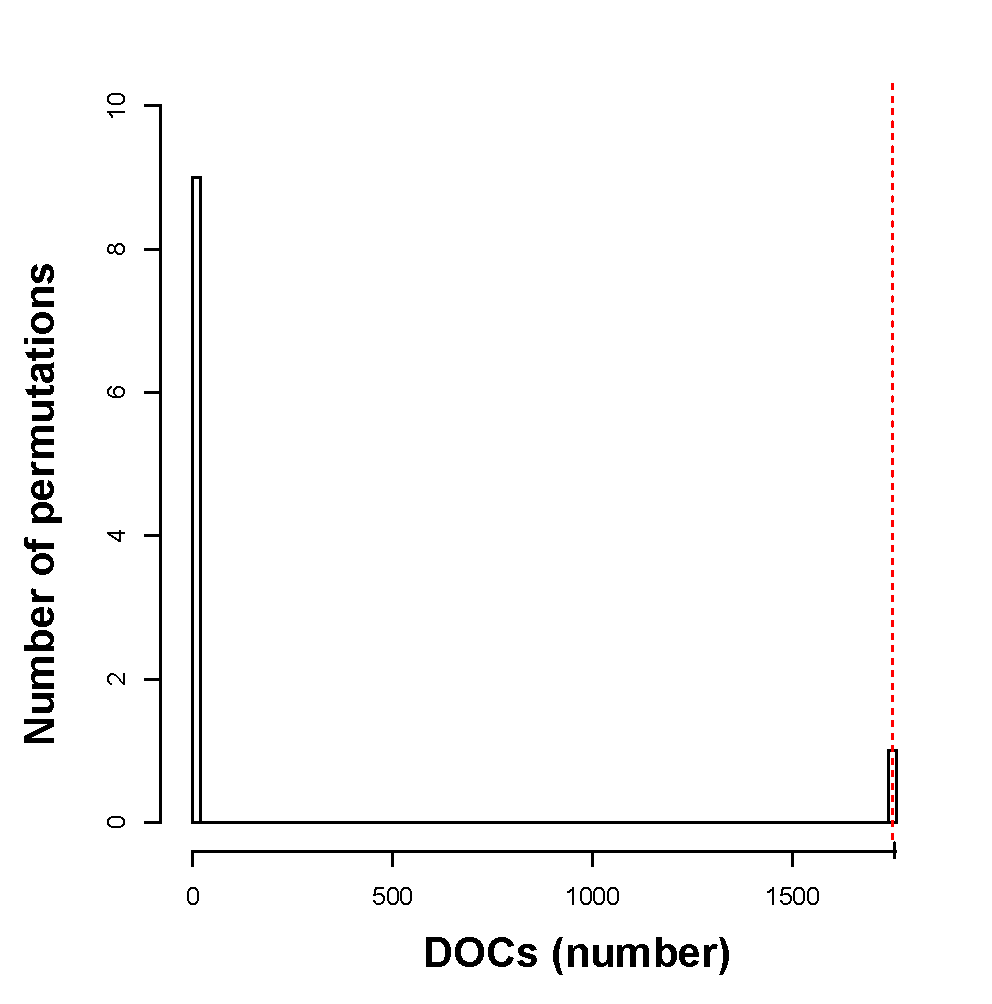
\includegraphics[width=\textwidth]{./Appendix/pdfs/Chapter5/ATAC_PsA_CD8_permutation_analysis}%
\caption{}
\end{subfigure}
\begin{subfigure}[b]{0.45\textwidth} 
%the [b] prevents offset in subcaptions
\centering
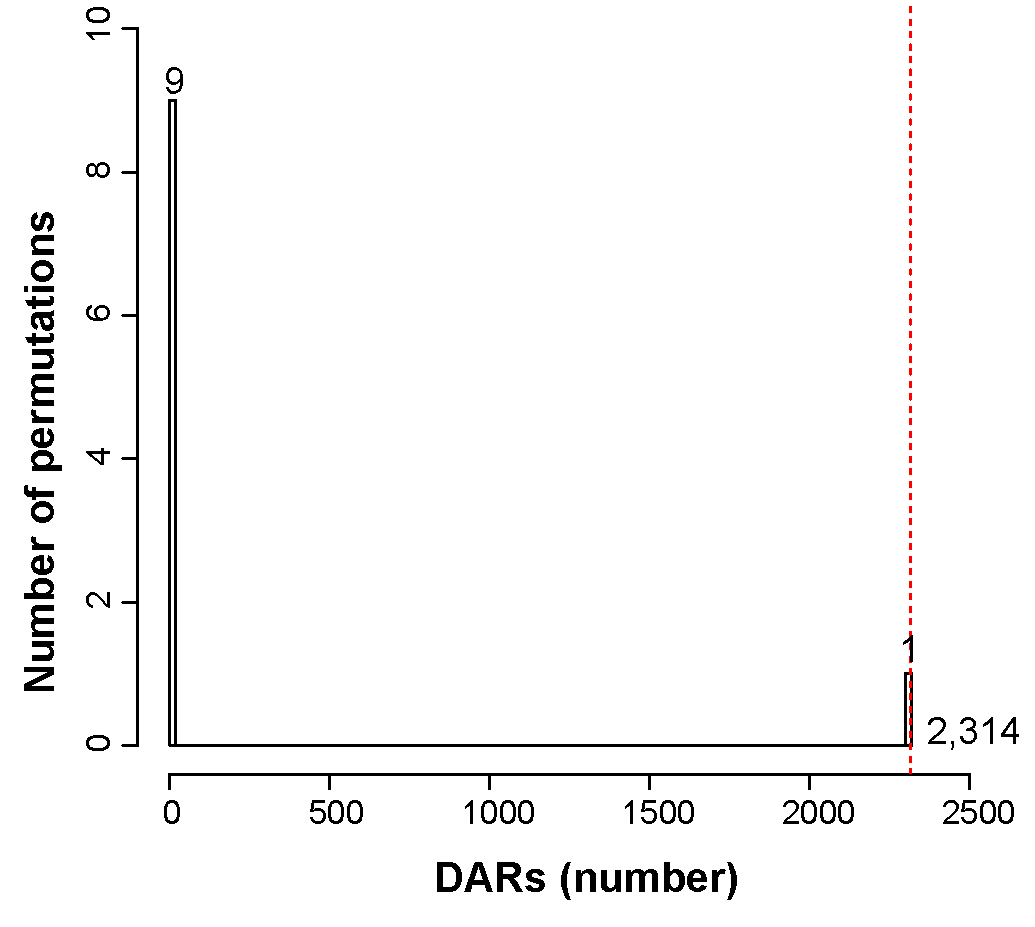
\includegraphics[width=\textwidth]{./Appendix/pdfs/Chapter5/ATAC_PsA_NK_permutation_analysis}%
\caption{}
\end{subfigure}
\caption[Permutation analysis for the DARs found in synovial vs peripheral blood in CD14$^+$ monocytes, mCD4$^+$, mCD8$^+$ and NK cells.]{\textbf{Permutation analysis for the DARs found in synovial vs peripheral blood in CD14$^+$ monocytes, mCD4$^+$, mCD8$^+$ and NK cells.} Sample labels were permuted within each cell type to achieve the ten unique possible combinations and differential analysis was performed. The number of significant DARs (FDR$<$0.01) across all permutations in plotted for (A) CD14$^+$ monocytes, (B) mCD4$^+$, (C) mCD8$^+$ and (D) NK cells, demonstrating that the true observation (dashed red line) is significantly more than expected by chance (p-value$<$0.1, the lowest p-value for the maximum number of permutations that can be conducted with this sample size) in all four cell types.}
\label{figure:PsA_perm_analysis}
\end{figure}


\begin{figure}[H]
\centering
\begin{subfigure}[b]{0.40\textwidth}
\centering 
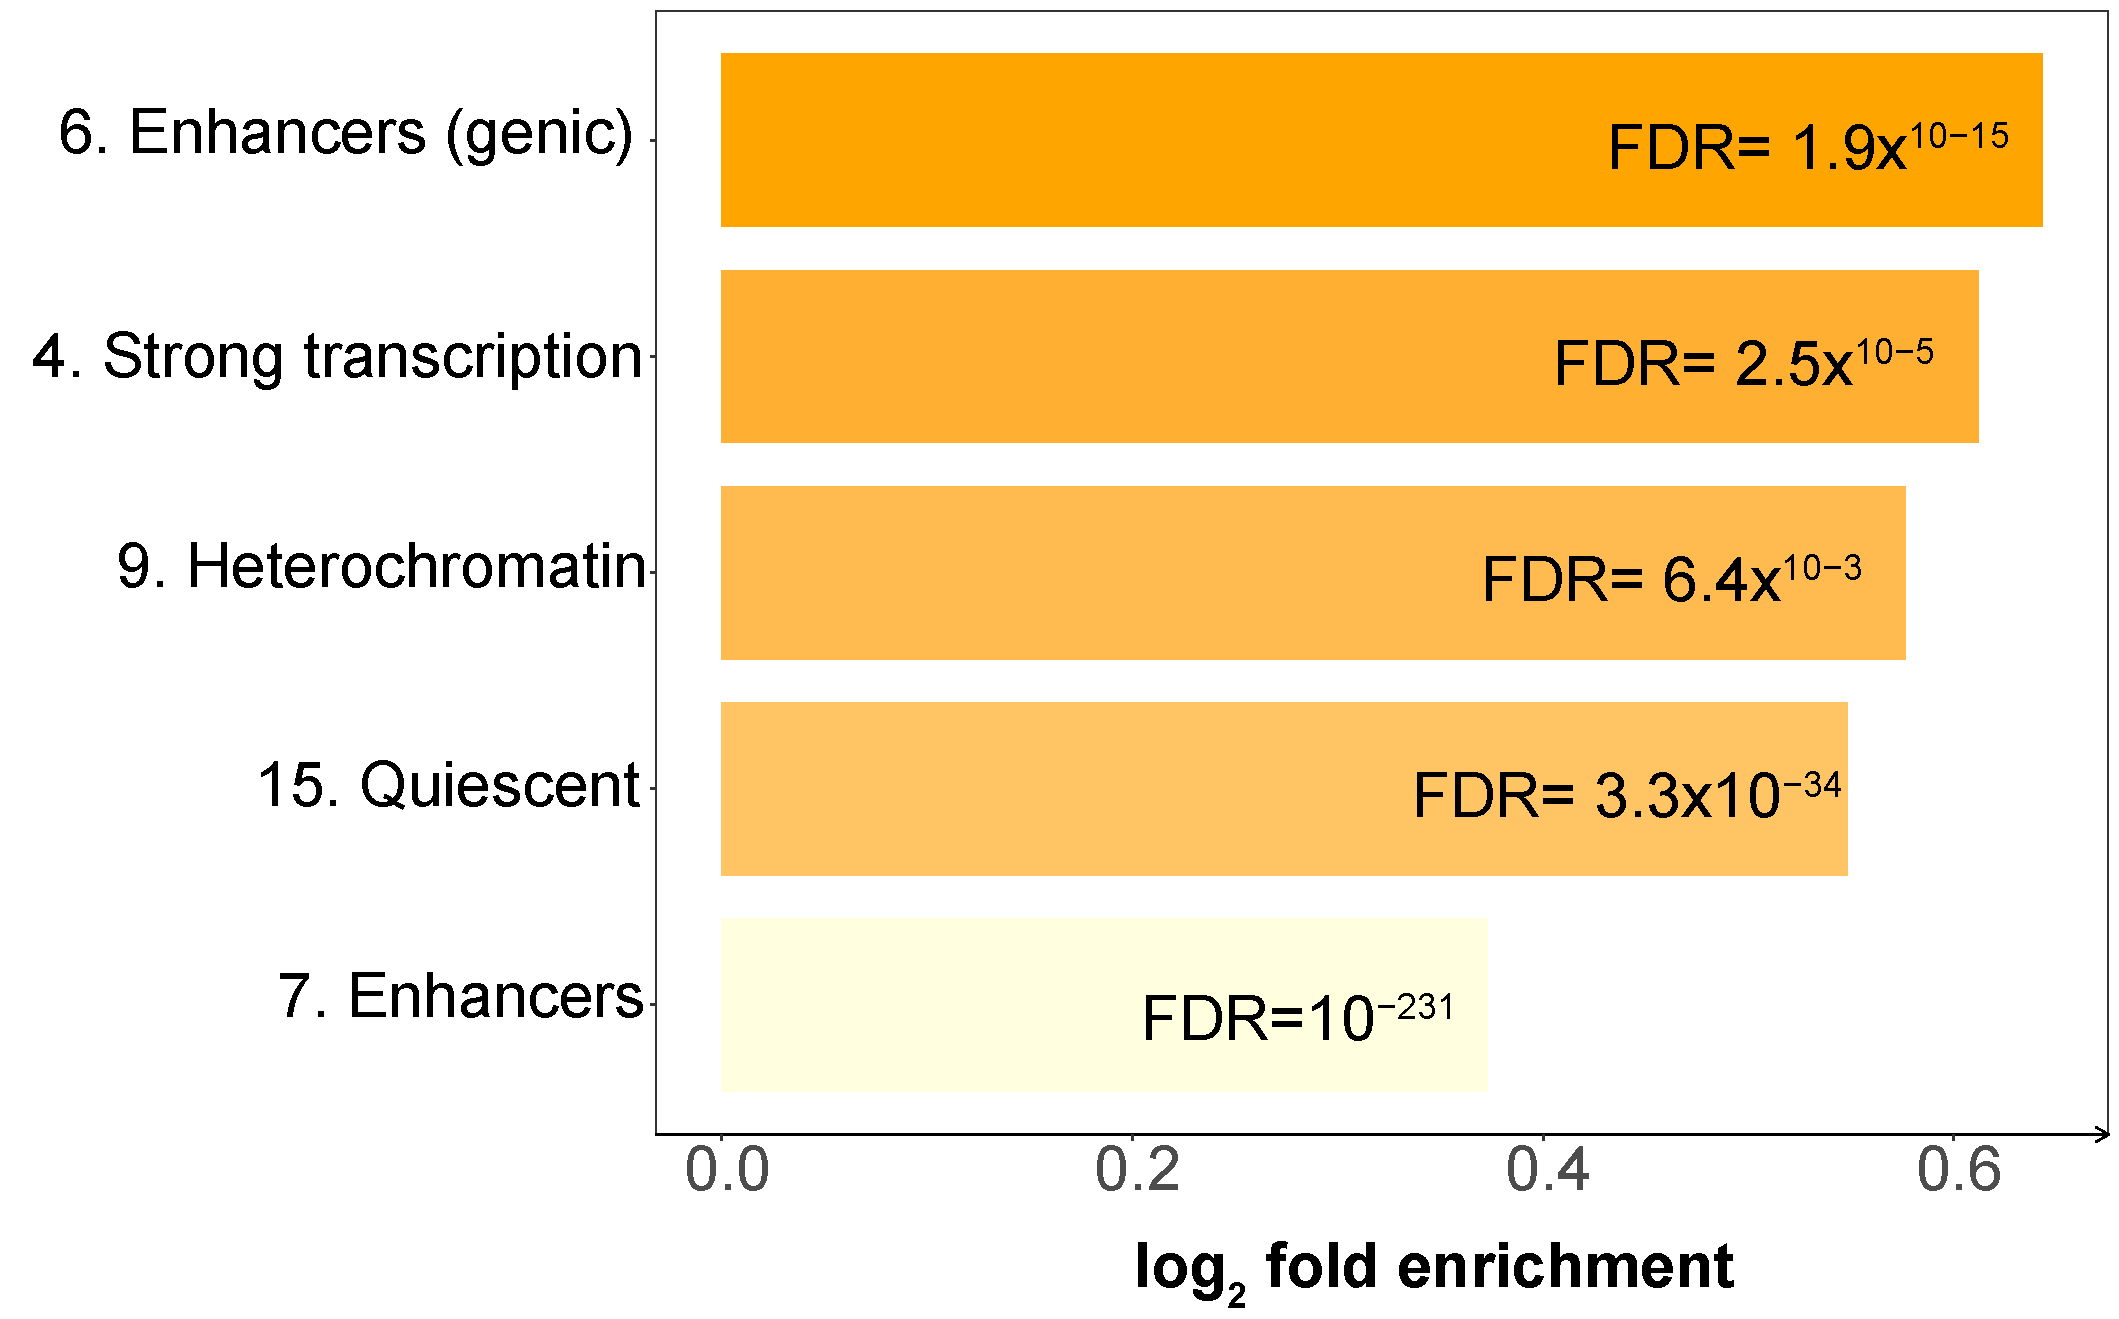
\includegraphics[width=\textwidth]{./Appendix/pdfs/Chapter5/ATAC_PSA_DAR_monocytes_chromatin_segments_enrichment_fc}
\caption{}
\end{subfigure}
~
\begin{subfigure}[b]{0.40\textwidth}
\centering 
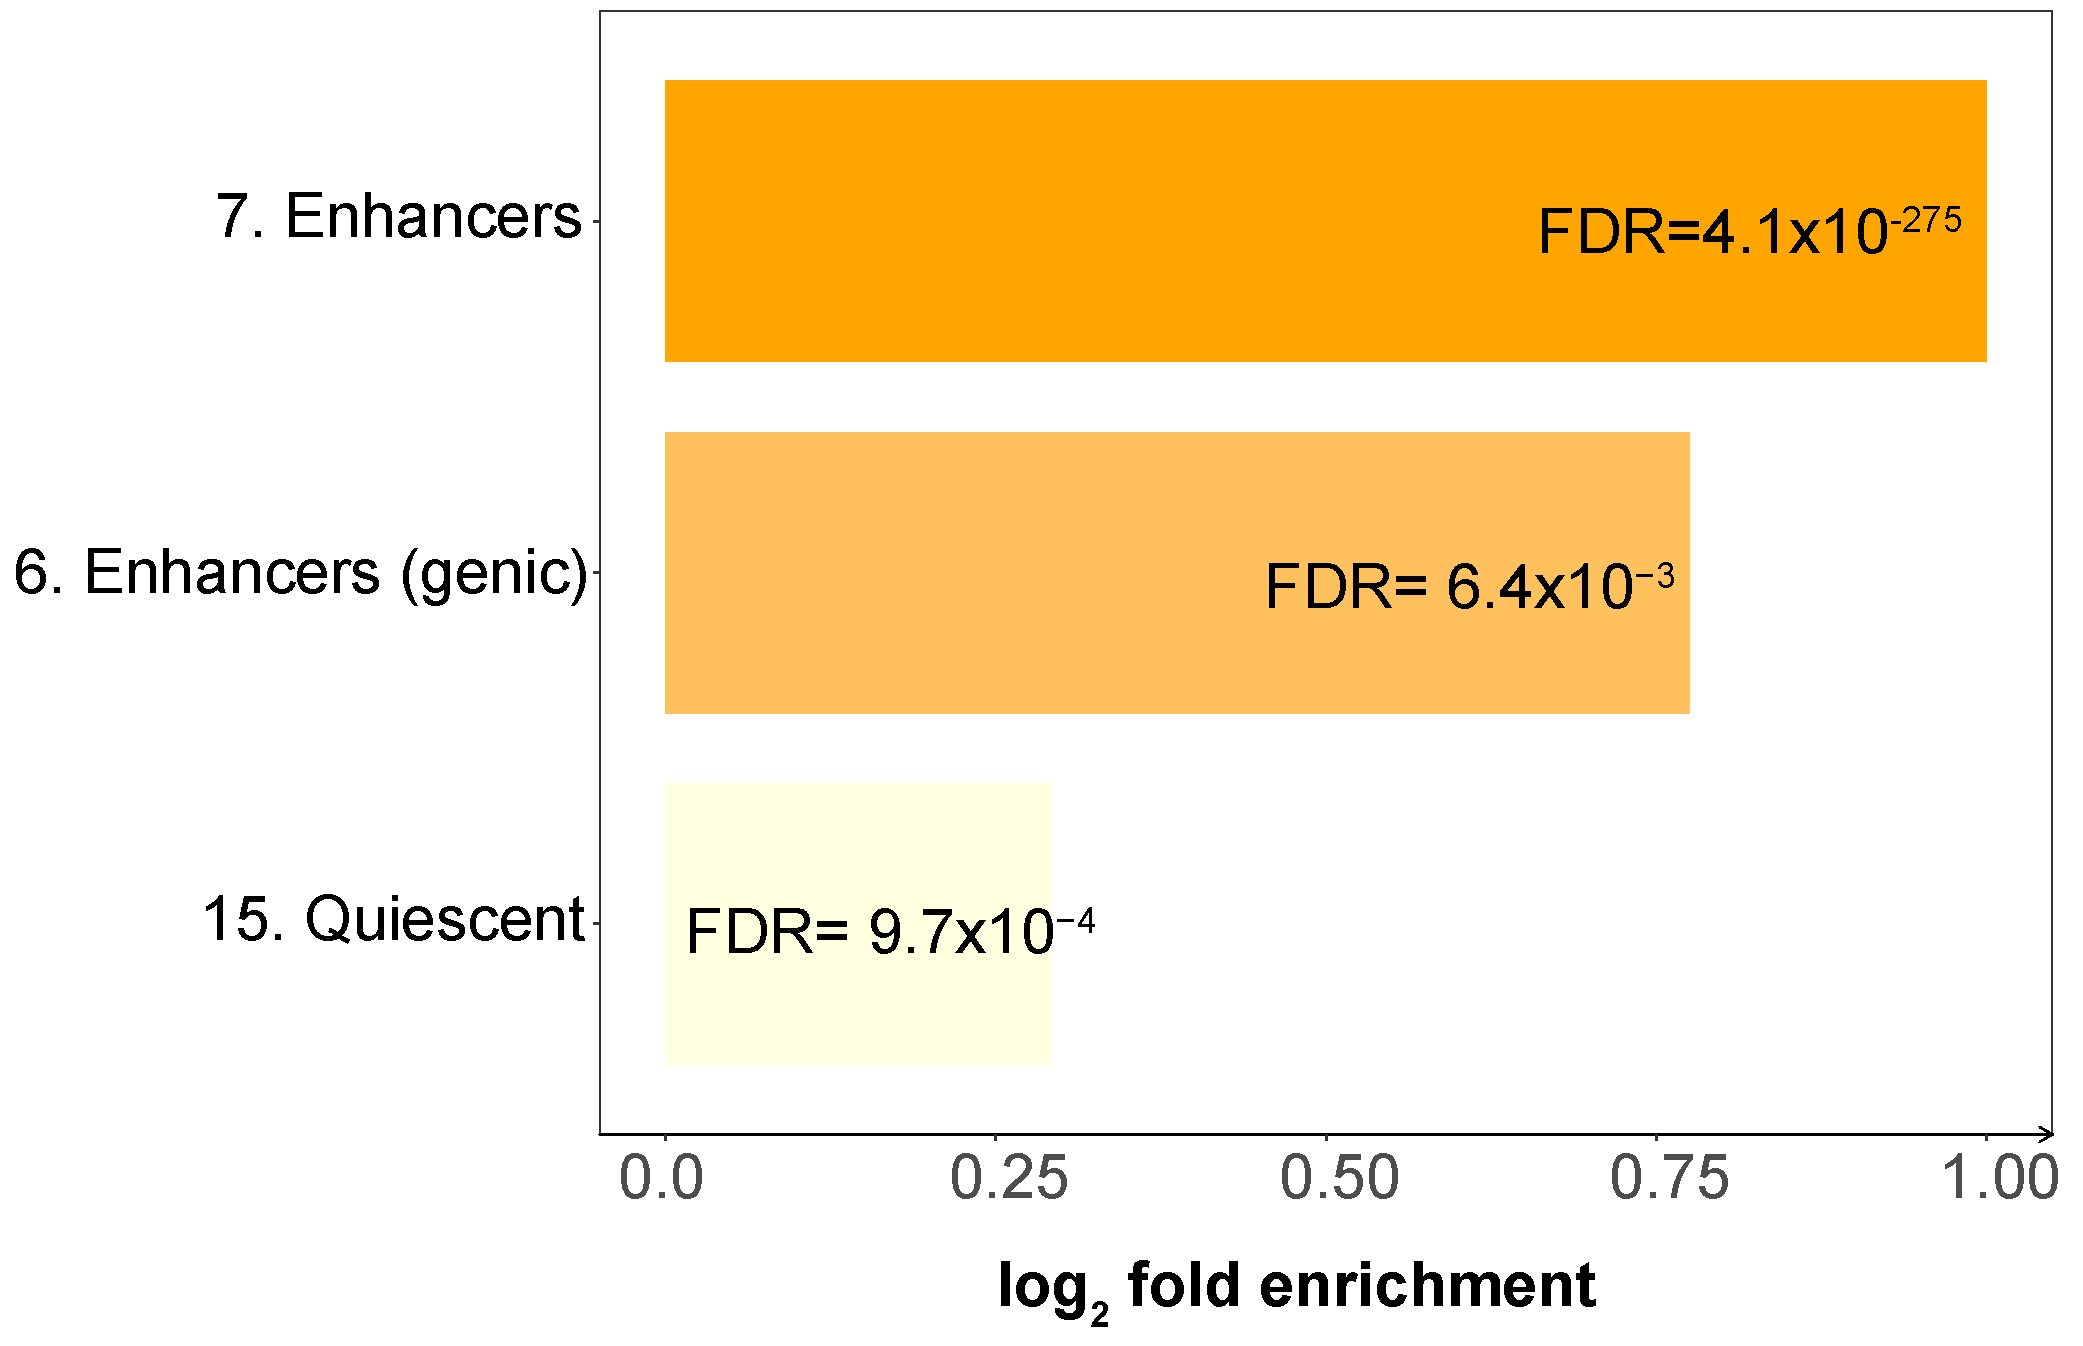
\includegraphics[width=\textwidth]{./Appendix/pdfs/Chapter5/ATAC_PSA_DAR_CD4_chromatin_segments_enrichment_fc}
\caption{}
\end{subfigure}
~
\begin{subfigure}[b]{0.40\textwidth} 
%the [b] prevents offset in subcaptions
\centering
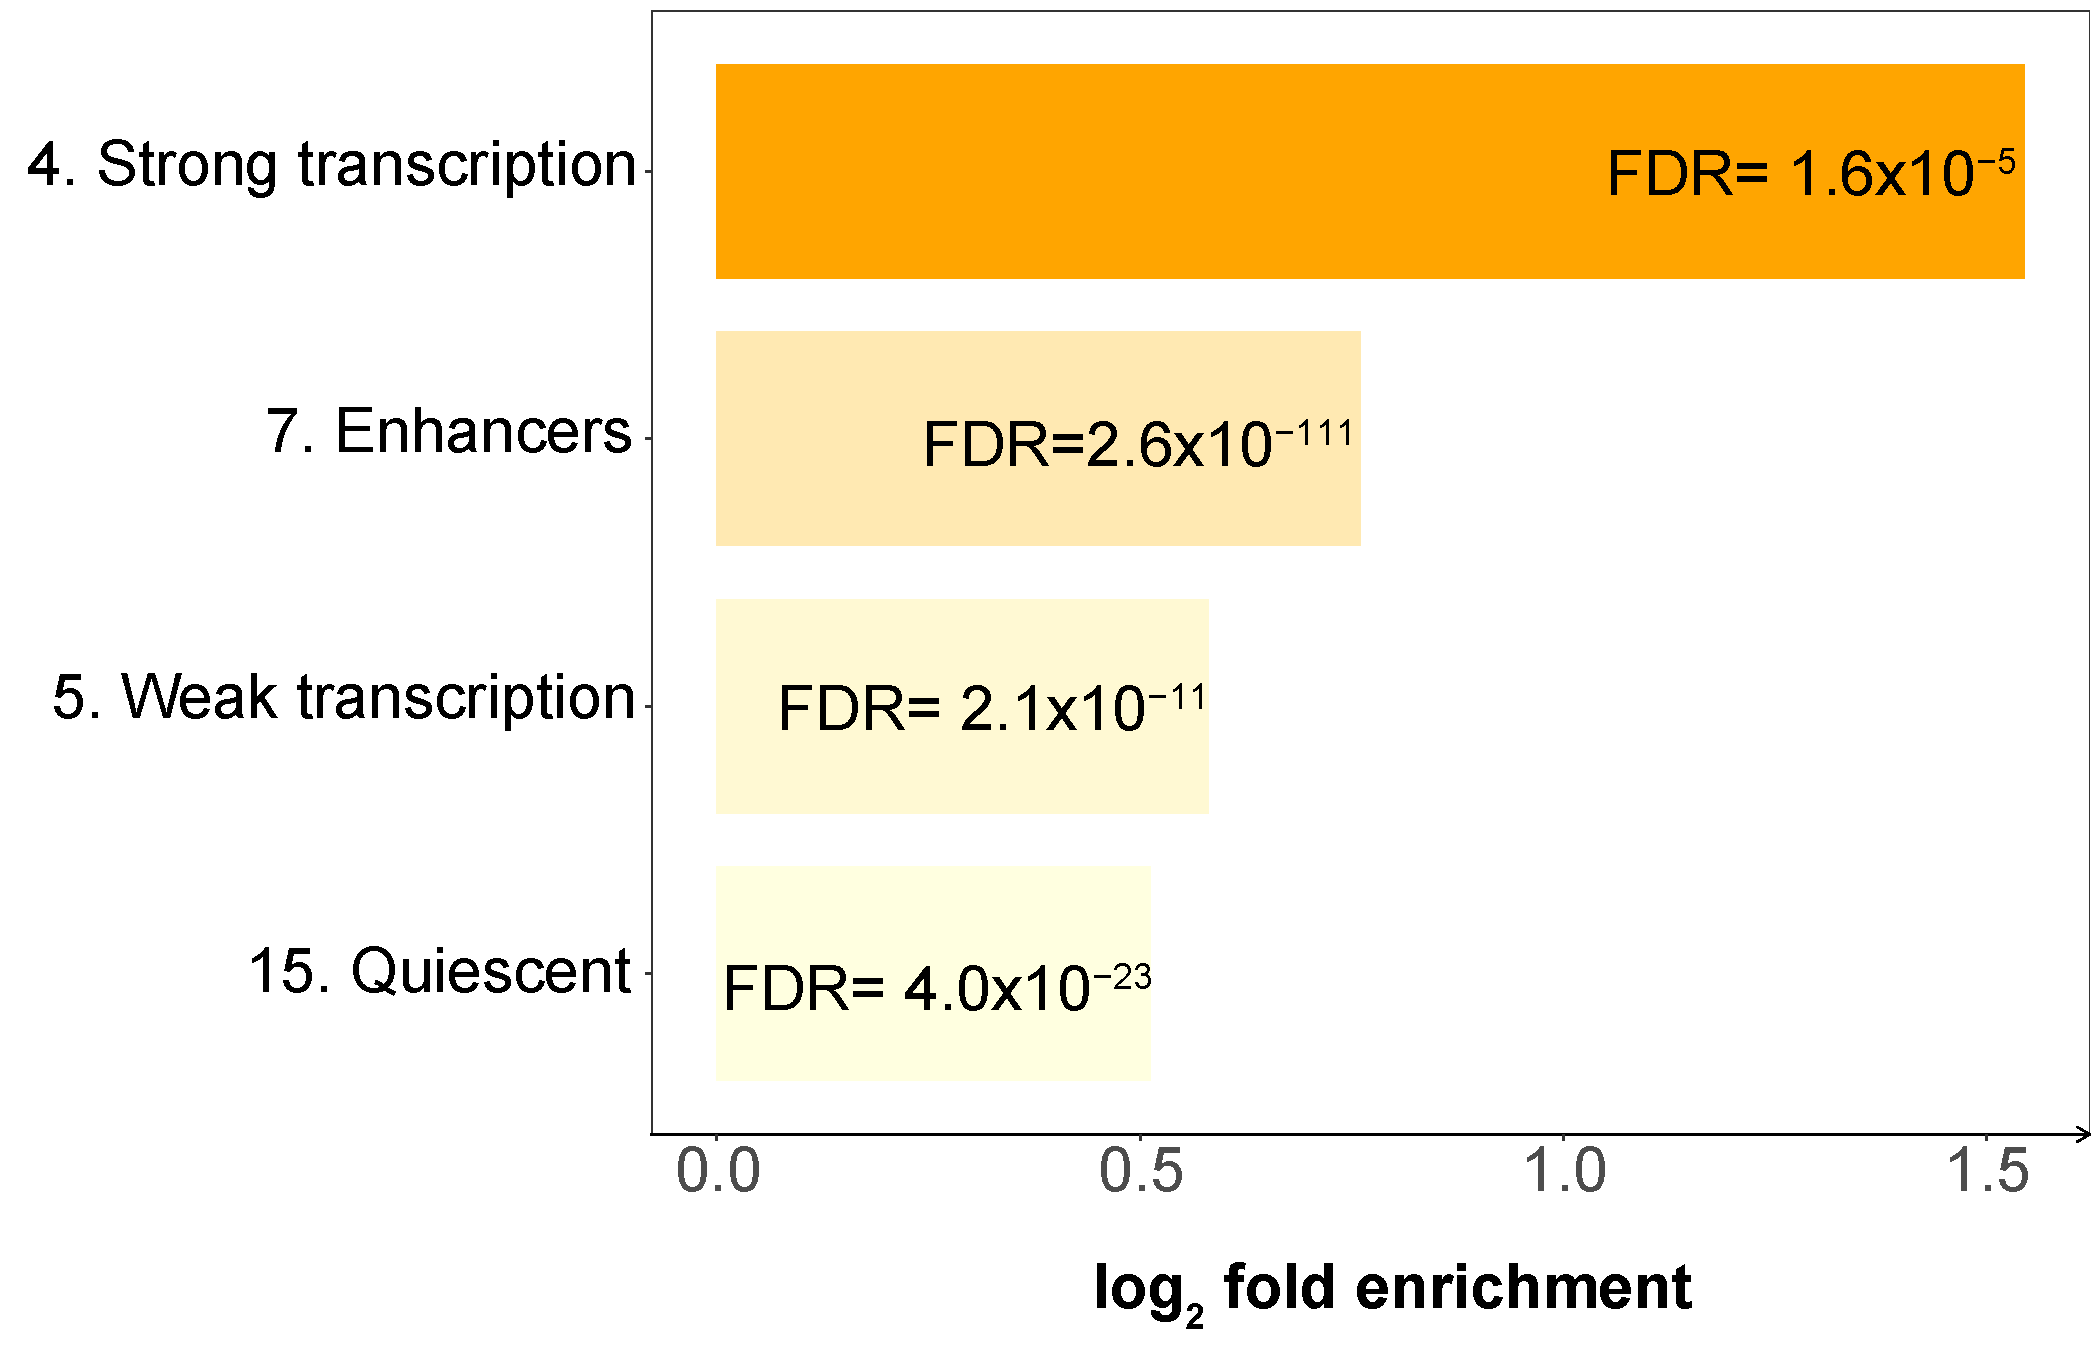
\includegraphics[width=\textwidth]{./Appendix/pdfs/Chapter5/ATAC_PSA_DAR_CD8_chromatin_segments_enrichment_fc}%
\caption{}
\end{subfigure}
\begin{subfigure}[b]{0.40\textwidth} 
%the [b] prevents offset in subcaptions
\centering
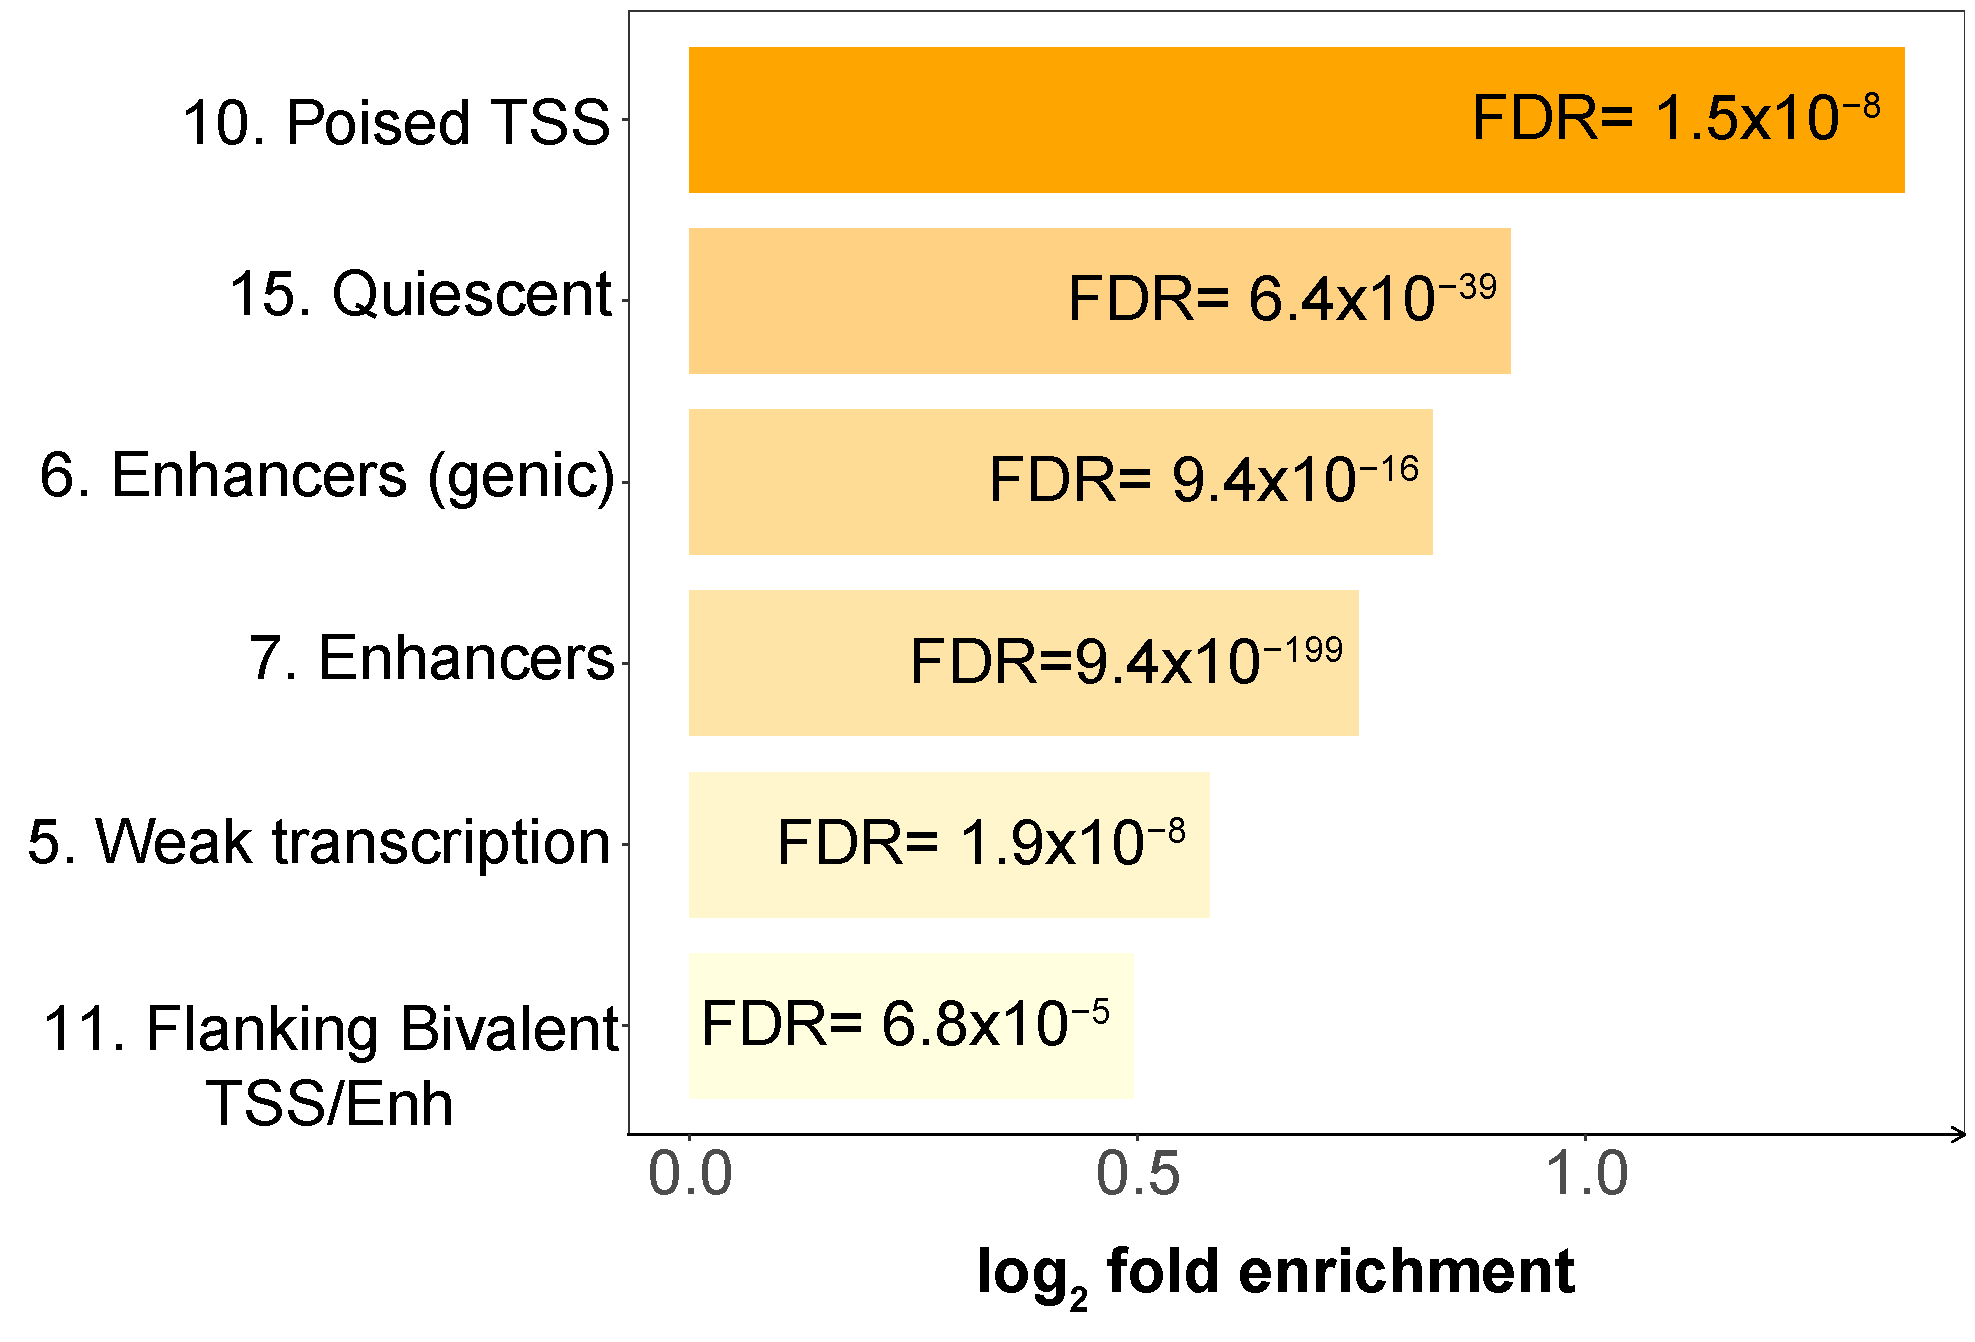
\includegraphics[width=\textwidth]{./Appendix/pdfs/Chapter5/ATAC_PSA_DAR_NK_chromatin_segments_enrichment_fc}%
\caption{}
\end{subfigure}
\caption[Enrichment of DARs in the 15 chromatin states of the cell type specific Roadmap Epigenomic Project segmentation maps.]{\textbf{Enrichment of DARs in the 15 chromatin states of the cell type specific Roadmap Epigenomic Project segmentation maps.} Barplots illustrating the chromatin states significantly enriched (FDR$<$0.01) in DARs from the differential chromatin accessibility analysis between synovial fluid and peripheral blood in (A) CD14$^+$ monocytes, (B) mCD4$^+$, (C) mCD8$^+$ and (D) NK cells. For each of the enriched chromatin states the statistical significance (FDR) and the magnitude (log$_2$ fold change) of the enrichment is included.}
\label{figure:PSA_ATAC_DARs_chromatin_states_enrichment}
\end{figure}


\bigskip
\begin{figure}[htbp]
\centering
\begin{subfigure}[b]{0.48\textwidth}
\centering 
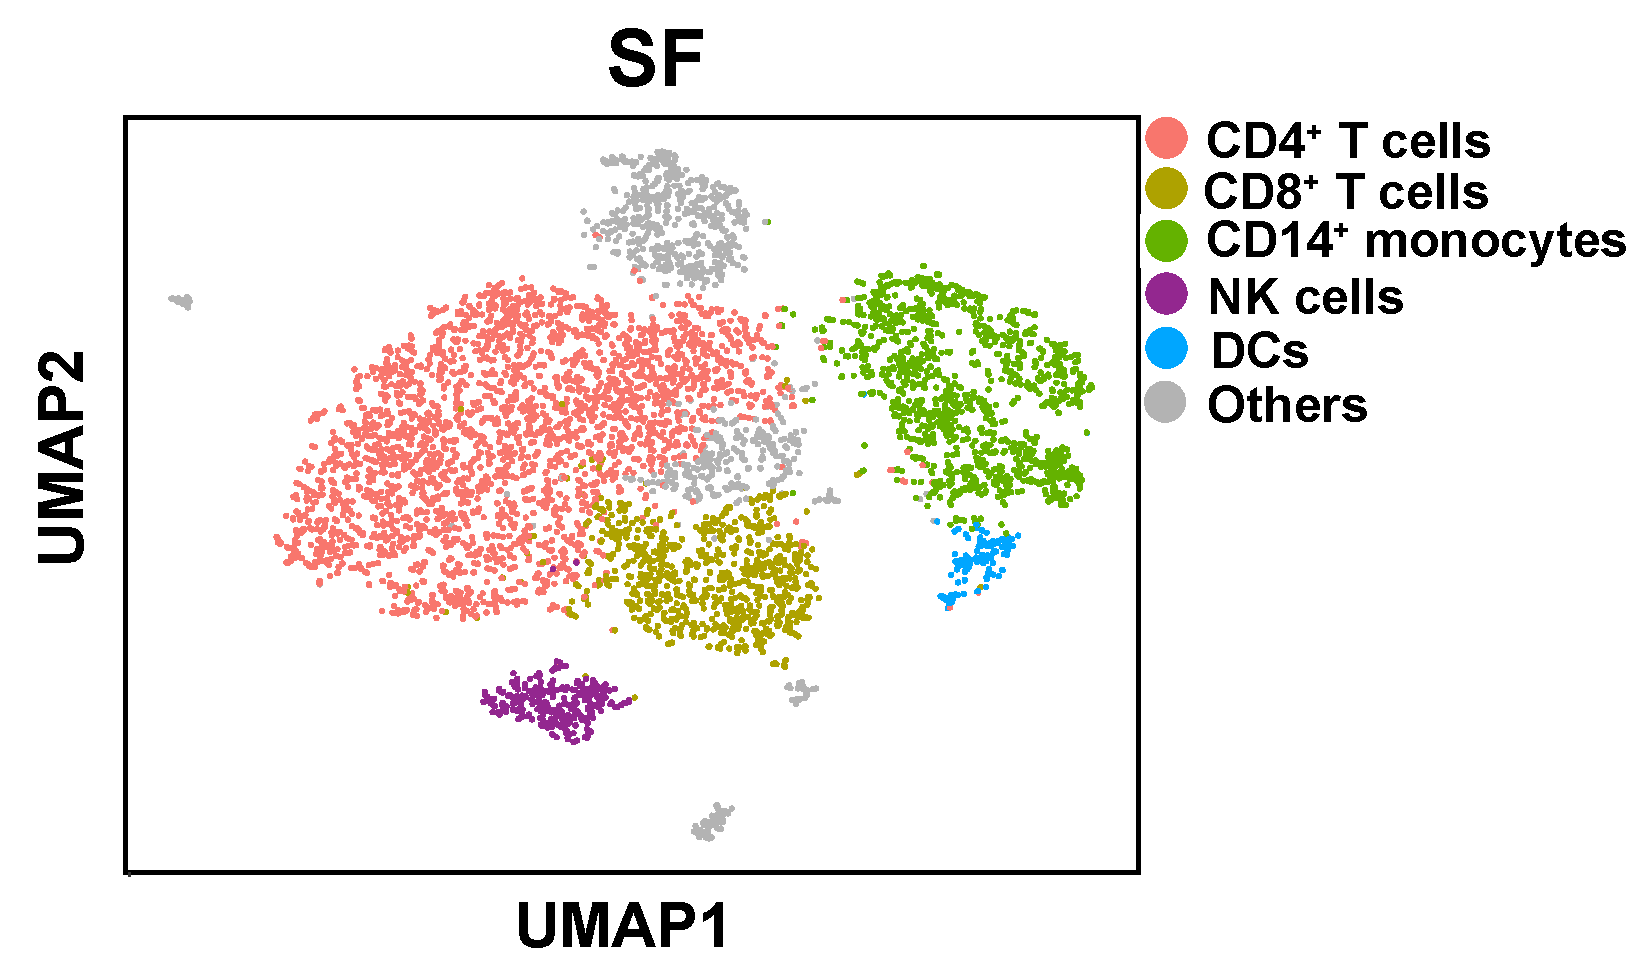
\includegraphics[width=\textwidth]{./Appendix/pdfs/Chapter5/PSA_monocytes_scanpy_single_cell_SF_all_cell_types}
\caption{}
\end{subfigure}%
~
\begin{subfigure}[b]{0.48\textwidth} 
%the [b] prevents offset in subcaptions
\centering
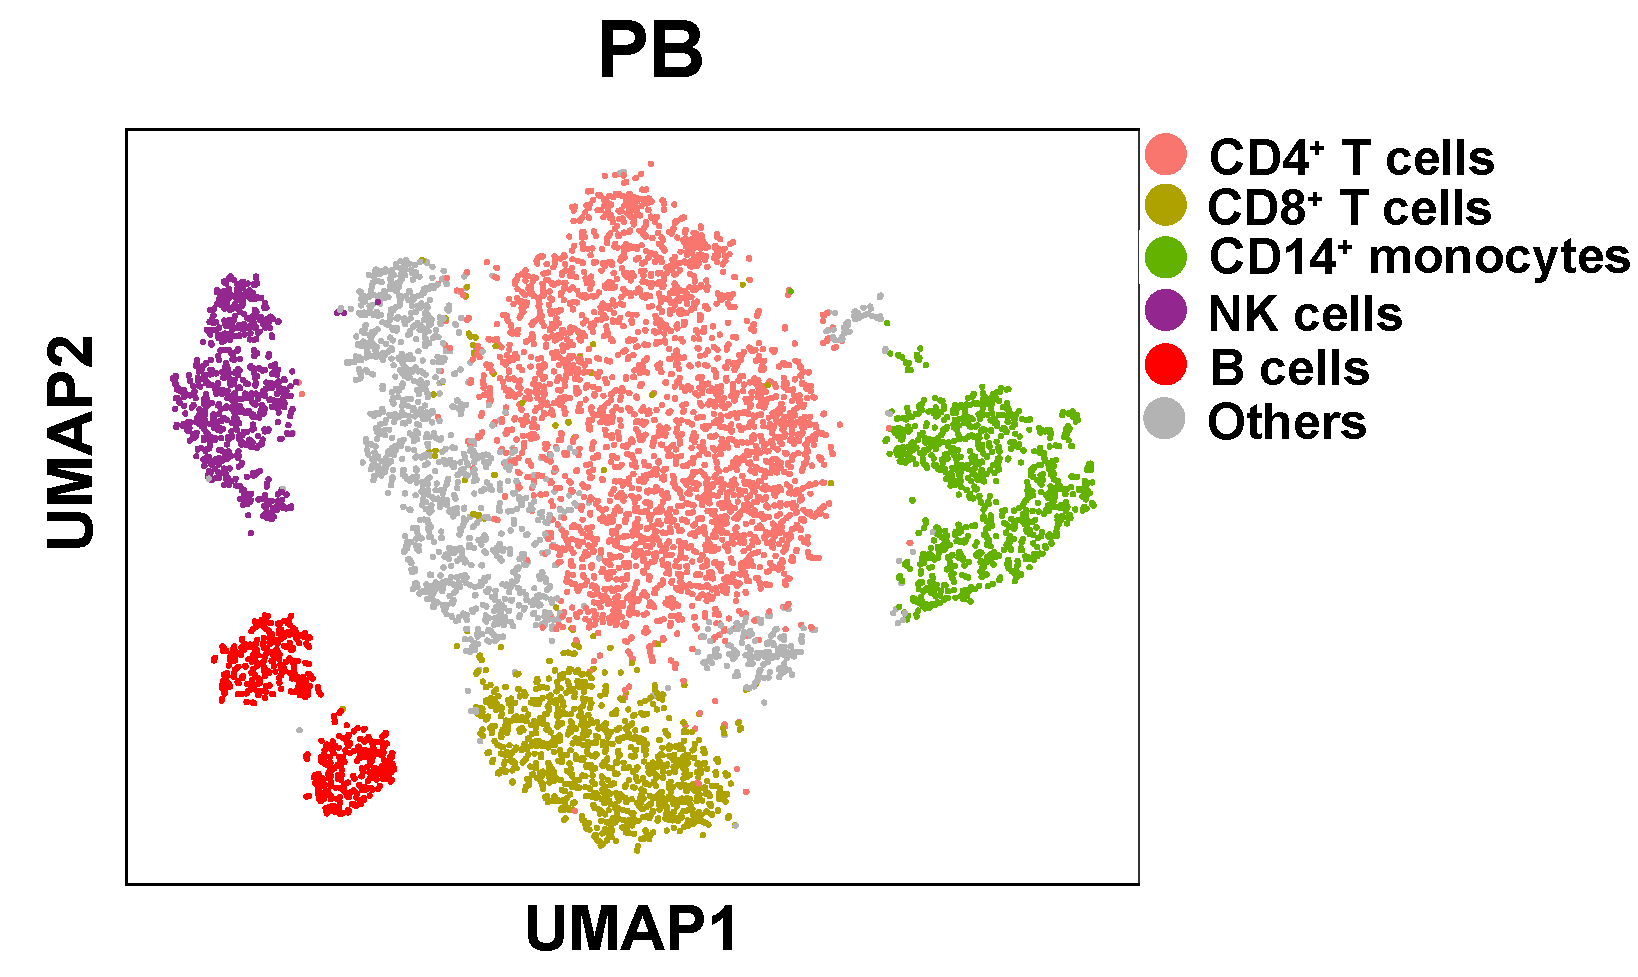
\includegraphics[width=\textwidth]{./Appendix/pdfs/Chapter5/PSA_monocytes_scanpy_single_cell_PB_all_cell_types}
\caption{}
\end{subfigure}
\caption[Identification of the CD14$^+$ monocytes populations from bulk SFMCs and PBMCs using scRNA-seq transcriptomes.]{\textbf{Identification of the CD14$^+$ monocytes populations from bulk SFMCs and PBMCs using scRNA-seq transcriptomes.} Visualisation using UMAP dimensional reduction of the cell type populations identified in (A) SFMCs and (B) PBMCs for a representative PsA sample. Clustering performed using default resolution allowed to identify CD4$^+$ (pink), CD8$^+$ (khaki), CD14$^+$ monocytes (green), NK (purple), DCs (blue), B cells (red) and others (grey).}
\label{figure:PsA_scRNAseq_SF_an_PB_monocytes_identification_from_bulk}
\end{figure}



\bigskip
\begin{figure}[ht]
\centering
\begin{subfigure}[b]{0.48\textwidth}
\centering 
\includegraphics[width=\textwidth]{./Appendix/pdfs/Chapter5/PSA_scanpy_single_cell_HLAD_vln_and_overlaid_markers}
\caption{}
\end{subfigure}%
~
\begin{subfigure}[b]{0.48\textwidth} 
%the [b] prevents offset in subcaptions
\centering
\includegraphics[width=\textwidth]{./Appendix/pdfs/Chapter5/PSA_scanpy_single_cell_phagocytosis_vln_and_overlaid_markers}
\caption{}
\end{subfigure}
\caption[Expression levels of antigen presentation and phagocytosis characteristic genes in synovial fluid and peripheral blood CD14$^+$ monocytes.]{\textbf{Expression levels of antigen presentation and phagocytosis characteristic genes in synovial fluid and peripheral blood CD14$^+$ monocytes.} Expression intensities of (A) MHC-II genes \textit{HLA-DRB1}, \textit{HLA-DRB5} and \textit{HLA-DPB1} and (B) the phagocytic markers \textit{CD36}, \textit{CD93} and \textit{CLEC4E}. On the left expression of each genes is overlaid on the UMAP dimensional reduction for the combined synovial fluid and peripheral blood CD14$^+$ monocytes analysed by scRNA-seq. On the right, violin plots illustrate for synovial fluid and peripheral blood CD14$^+$ monocytes (x-axis) the probability density of expression (y-axis) for each of the genes. SF=synovial fluid; PB=peripheral blood.}
\label{figure:PsA_scRNAseq_ag_presentation_phagocytosis}
\end{figure}




\begin{figure}[htbp]
\centering
\begin{subfigure}[b]{0.60\textwidth}
\centering 
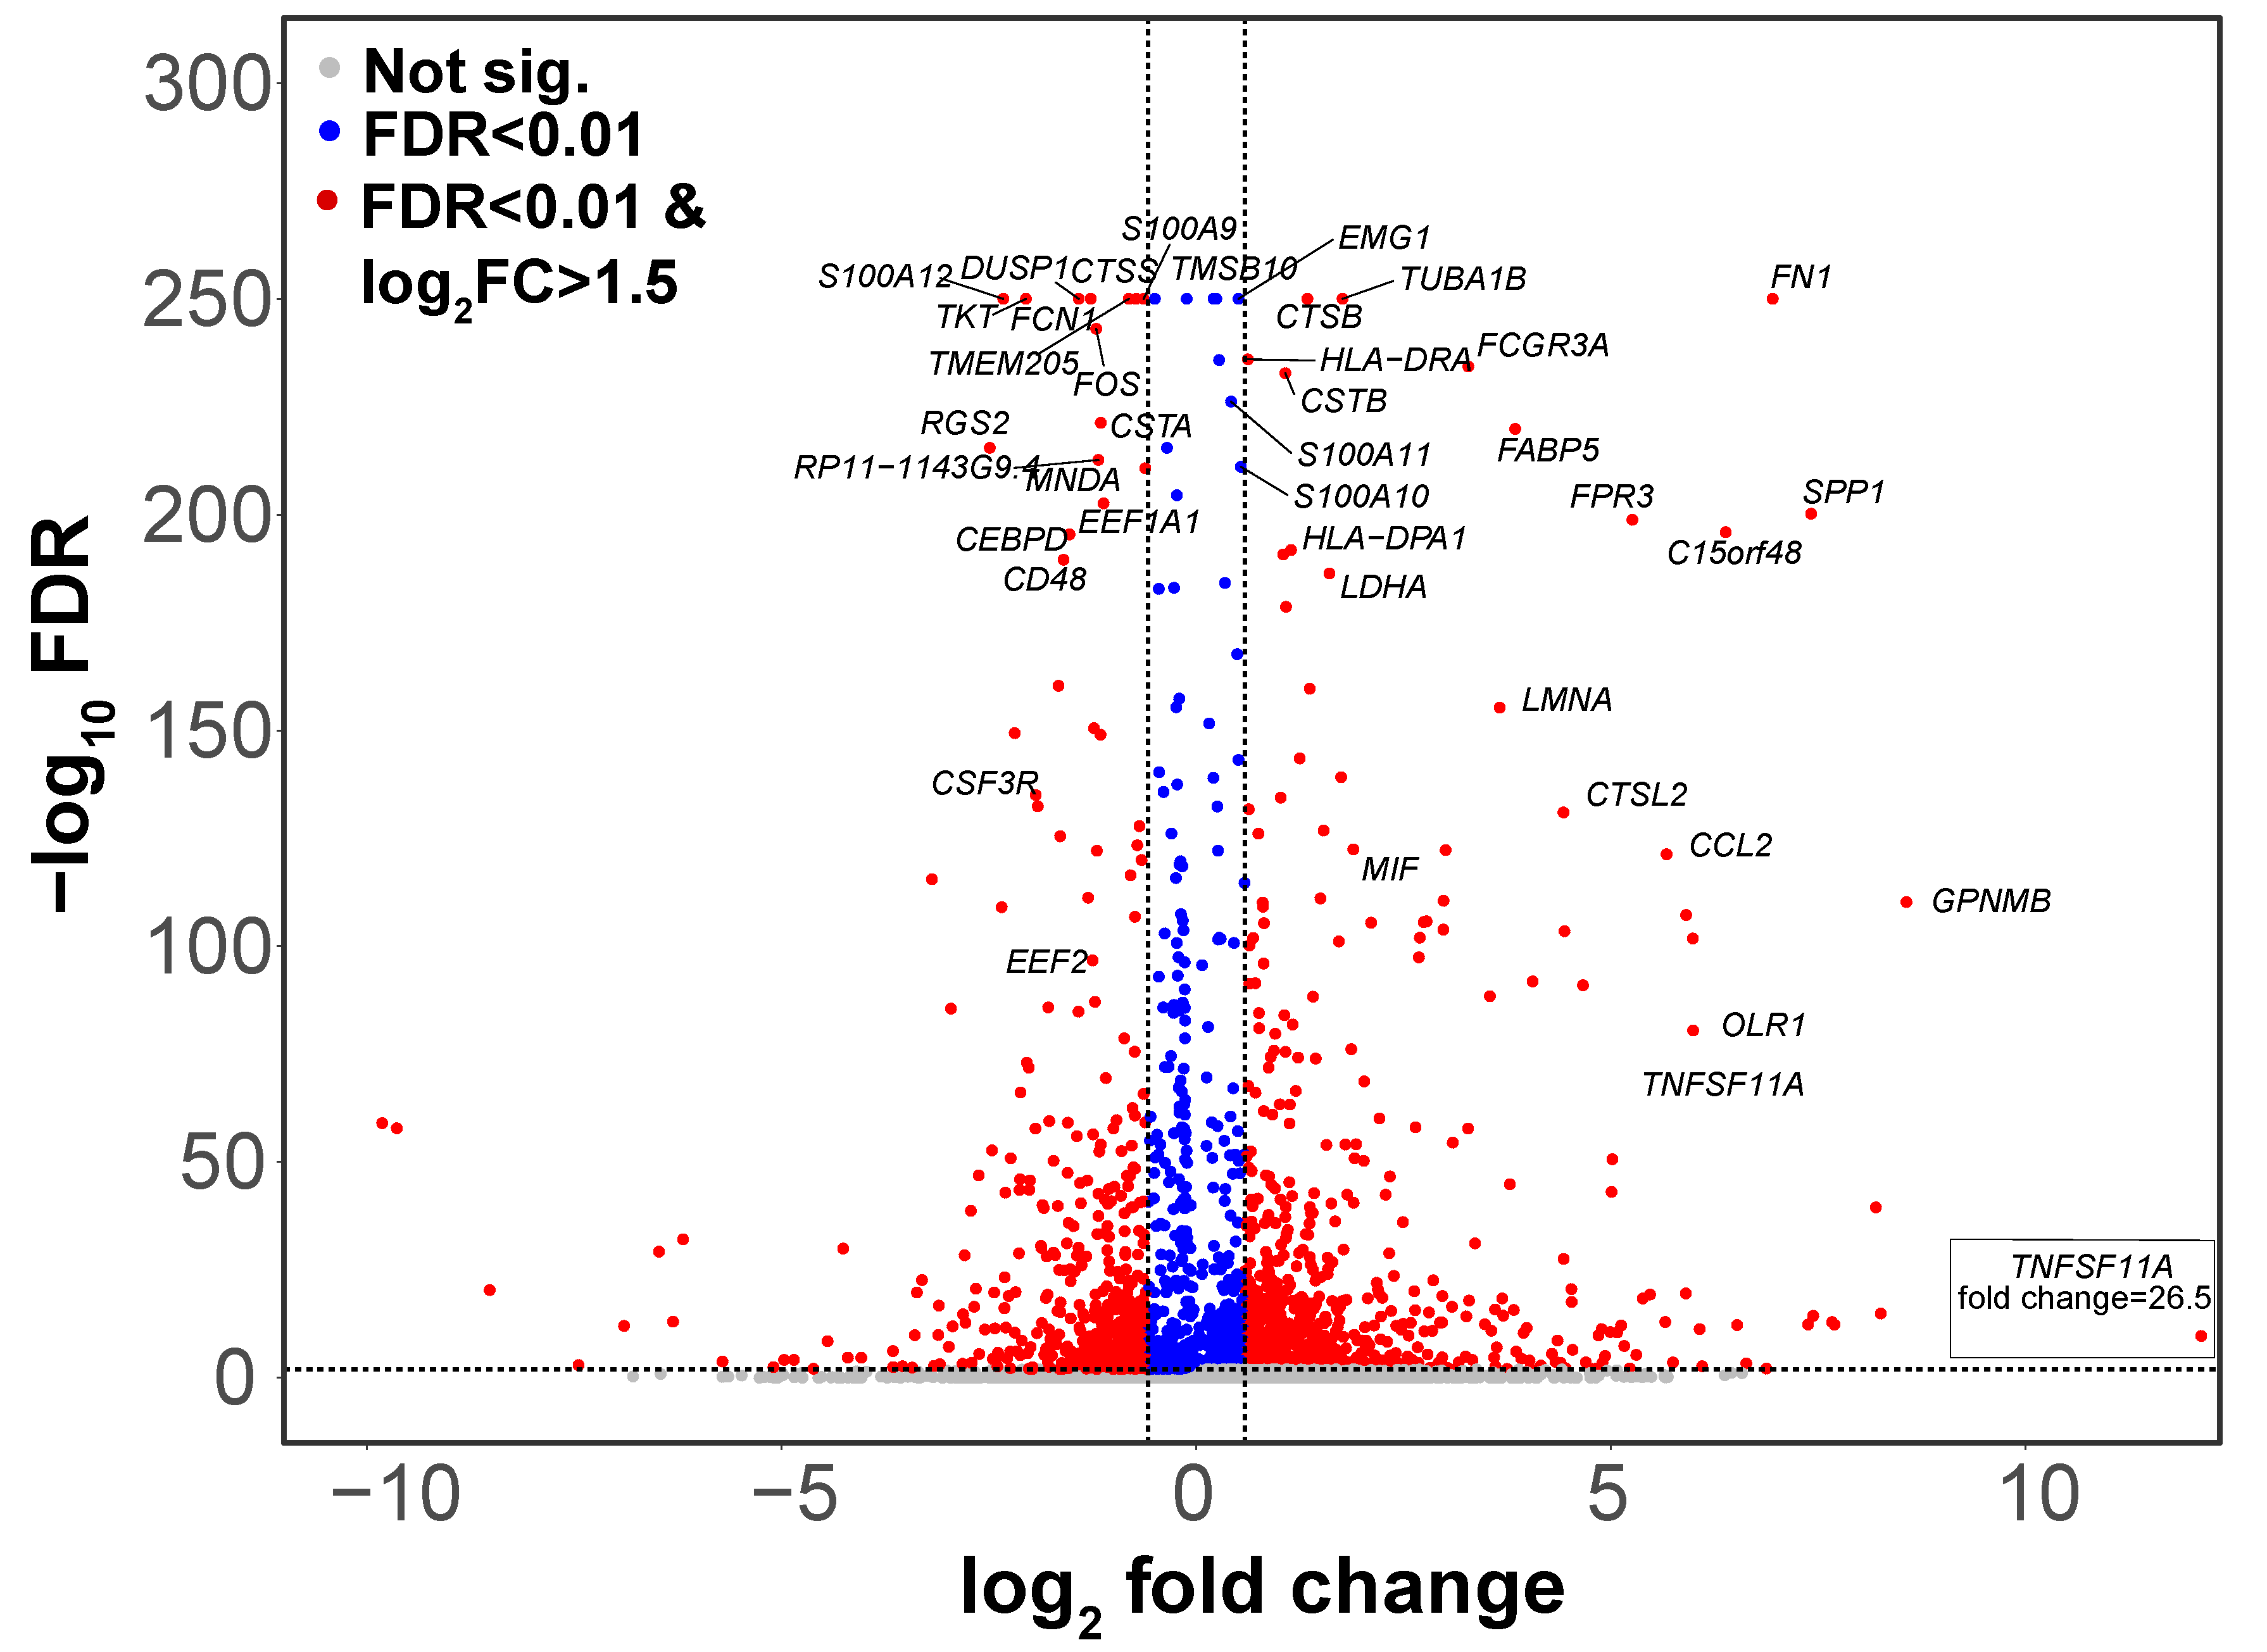
\includegraphics[width=\textwidth]{./Appendix/pdfs/Chapter5/PSA_monocytes_scanpy_single_cell_SFvsPB_volcano_plot_differential_analysis_less_labels}
\caption{}
\end{subfigure}
~
\begin{subfigure}[b]{0.50\textwidth}
\centering 
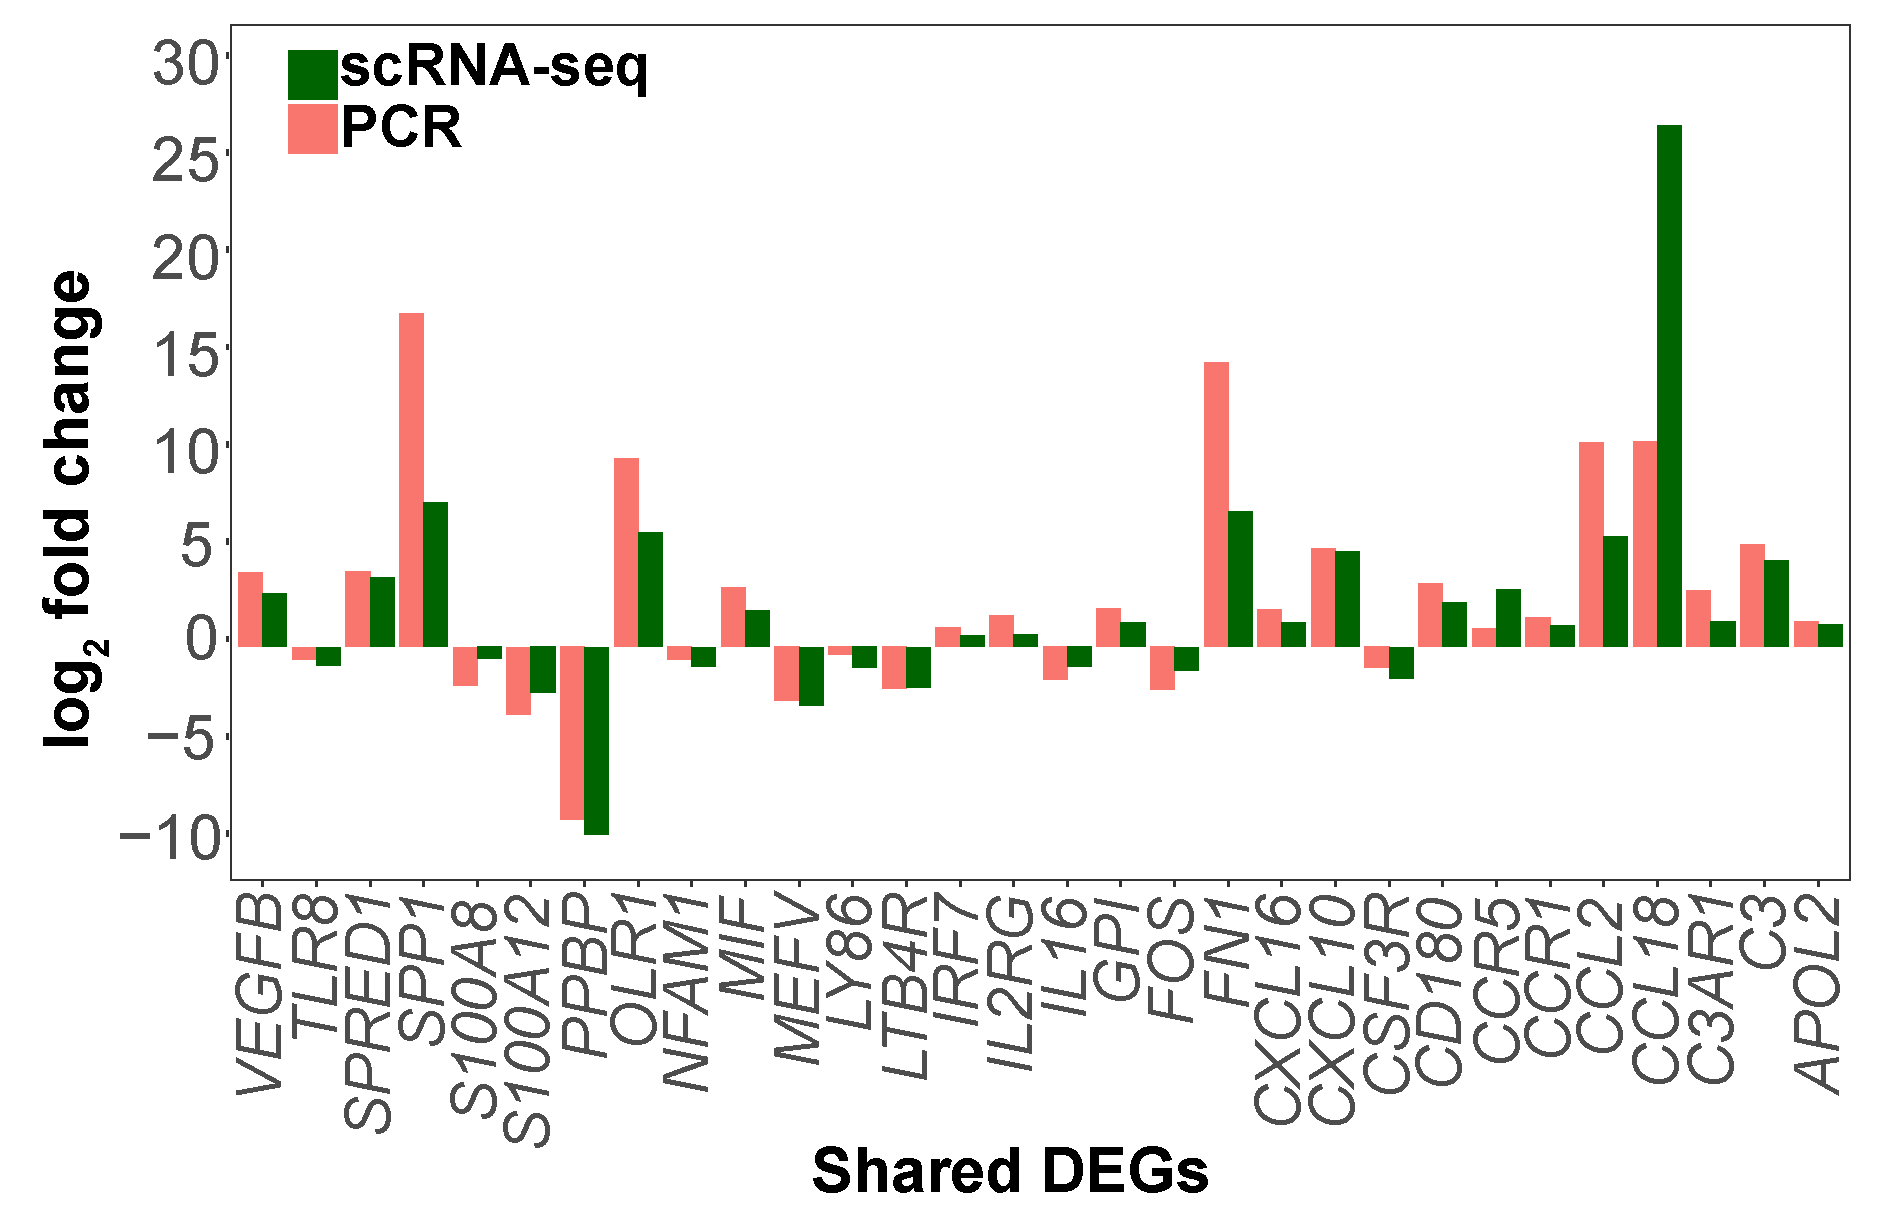
\includegraphics[width=\textwidth]{./Appendix/pdfs/Chapter5/PSA_monocytes_scanpy_single_cell_SFvsPB_PCR_correlation_fc_filtered}
\caption{}
\end{subfigure}%
~
\begin{subfigure}[b]{0.50\textwidth} 
%the [b] prevents offset in subcaptions
\centering
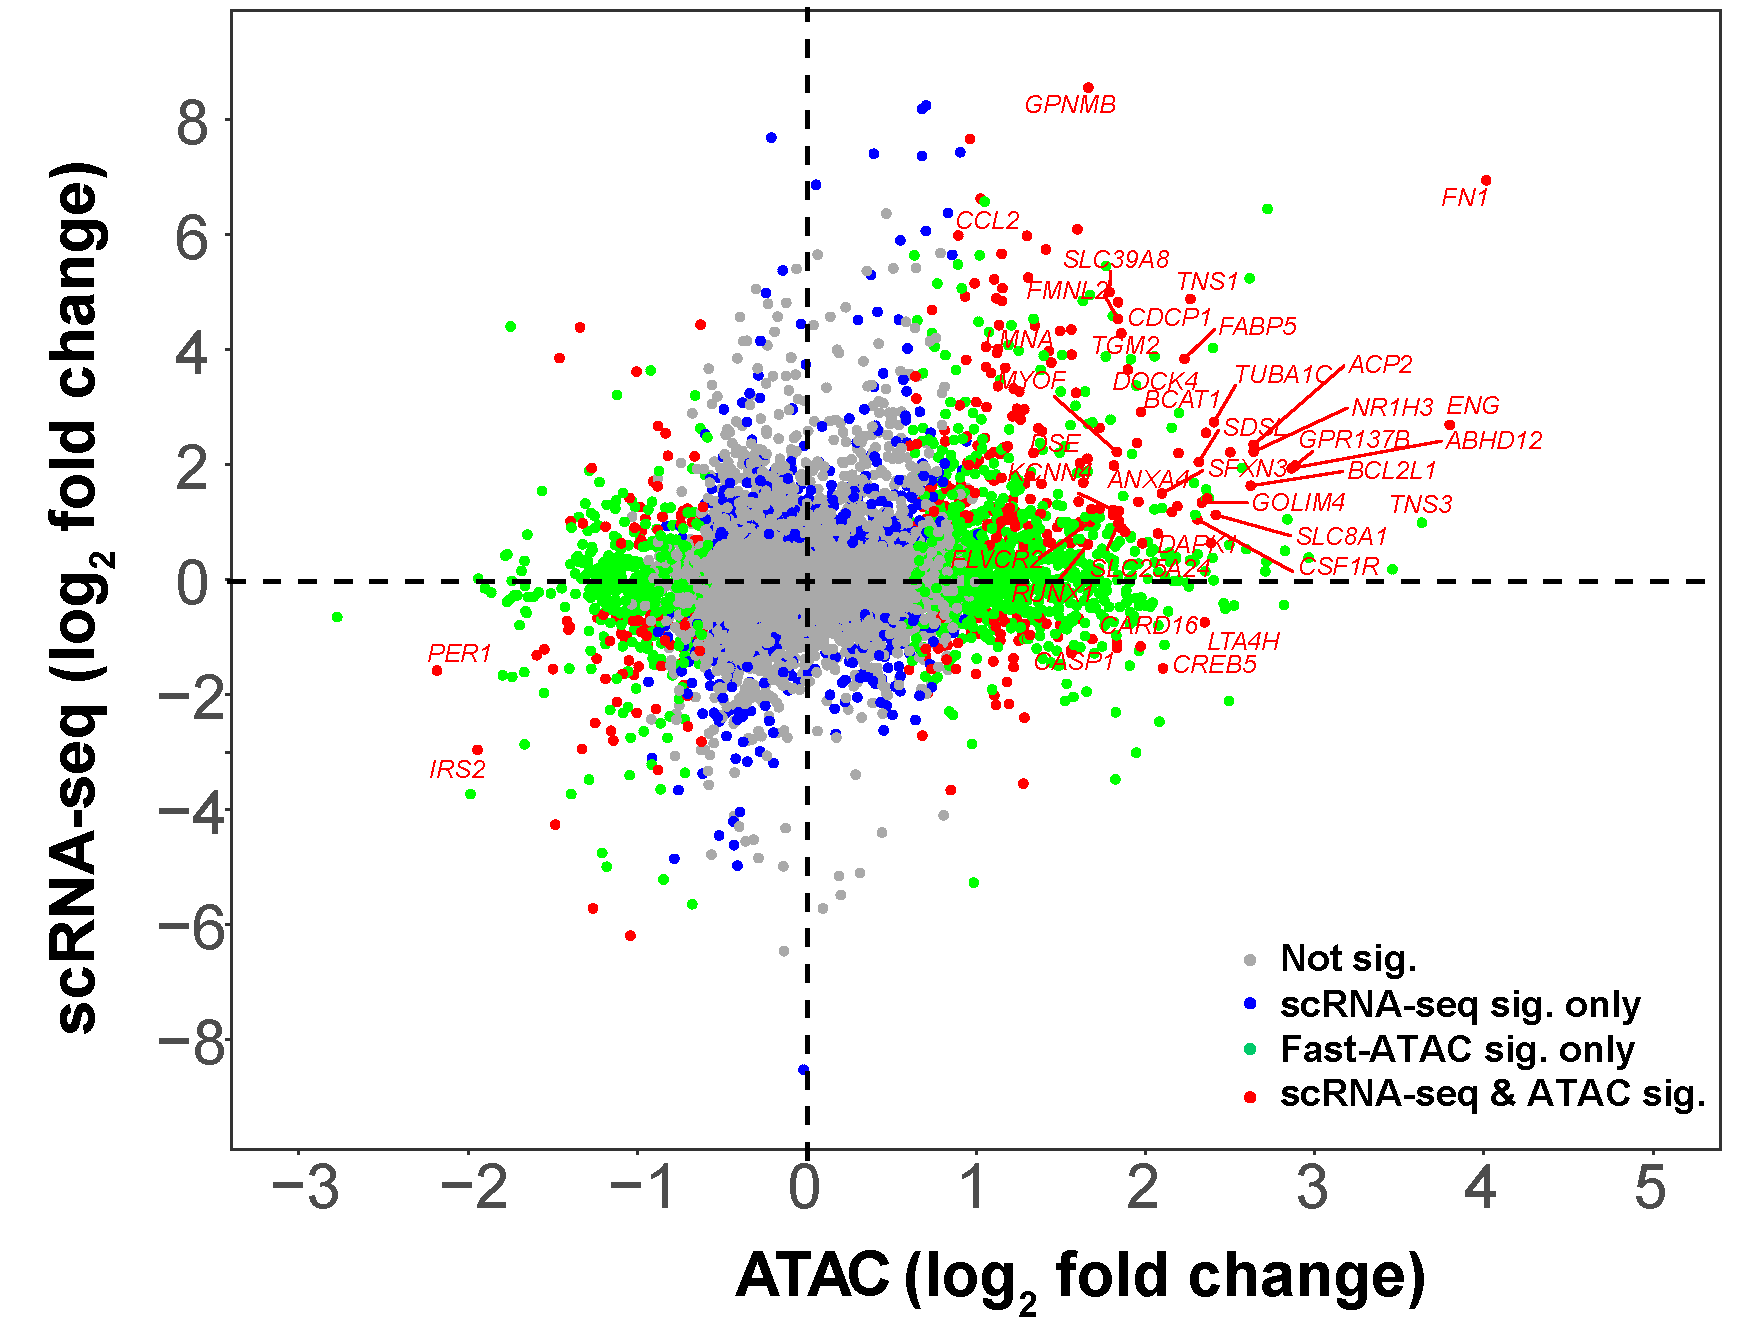
\includegraphics[width=\textwidth]{./Appendix/pdfs/Chapter5/PSA_monocytes_scanpy_single_cell_SFvsPB_scRNA_ATAC_corelation}
\caption{}
\end{subfigure}
\caption[Differential gene expression between synovial fluid and peripheral blood PsA CD14$^+$ monocytes and correlation with qPCR and chromatin accessibility]{\textbf{Correlation between scRNA-seq, qPCR and chromatin accessibility in PsA CD14$^+$ monocytes.} (A) Volcano plots showing differences in gene expression between synovial fluid and peripheral blood CD14$^+$ monocyte using scRNA-seq data. The significance (log$_{10}$FDR) of the differential expression (y-axis) is plotted against the log${_2}$ fold change, where a positive fold change indicates higher expression in CD14$^+$ monocytes from synovial fluid compared to peripheral blood and viceversa. Genes are coloured based on FDR and log$_{2}$fold changes and some of the top significant genes are labelled. (B) Comparison of the fold-changes for the shared DEGs between scRNA-seq and qPCR analysis of synovial fluid vs peripheral blood CD14$^+$ monocytes. The barplot illustrates the log$_2$fold change for the 30 DEGs identified by scRNA-seq (based on FDR$<$0.01 and fold change$>$1.5) and qPCR array (based on p-value$<$0.05) analysis. (C) Correlation plot comparing synovial fluid and peripheral blood differences in scRNA-seq expression and ATAC chromatin accessibility in CD14$^+$ monocytes. The log$_2$fold changes for scRNA-seq differential expression of all transcripts in CD14$^+$ monocytes are plotted against the log$_2$fold change for total CD14$^+$ monocytes ATAC differential chromatin accessibility analysis in regions proximal ($\leq$5Kb) to the same genes. Blue colouring indicates significant differential expression in scRNA-seq only; green represents ATAC significant DAR only; red indicates significant differential expression and chromatin accessibility; grey indicates no significant differential expression or chromatin accessibility in CD14$^+$ monocytes. Significance is based on FDR and fold change thresholds (FDR$<$0.01 and fold change$>$1.5) in both assays.}
\label{figure:PSA_monocytes_scanpy_single_cell_volcano_and_qPCR_ATAC_correlation}
\end{figure}

%\begin{figure}[htbp]
%\centering
%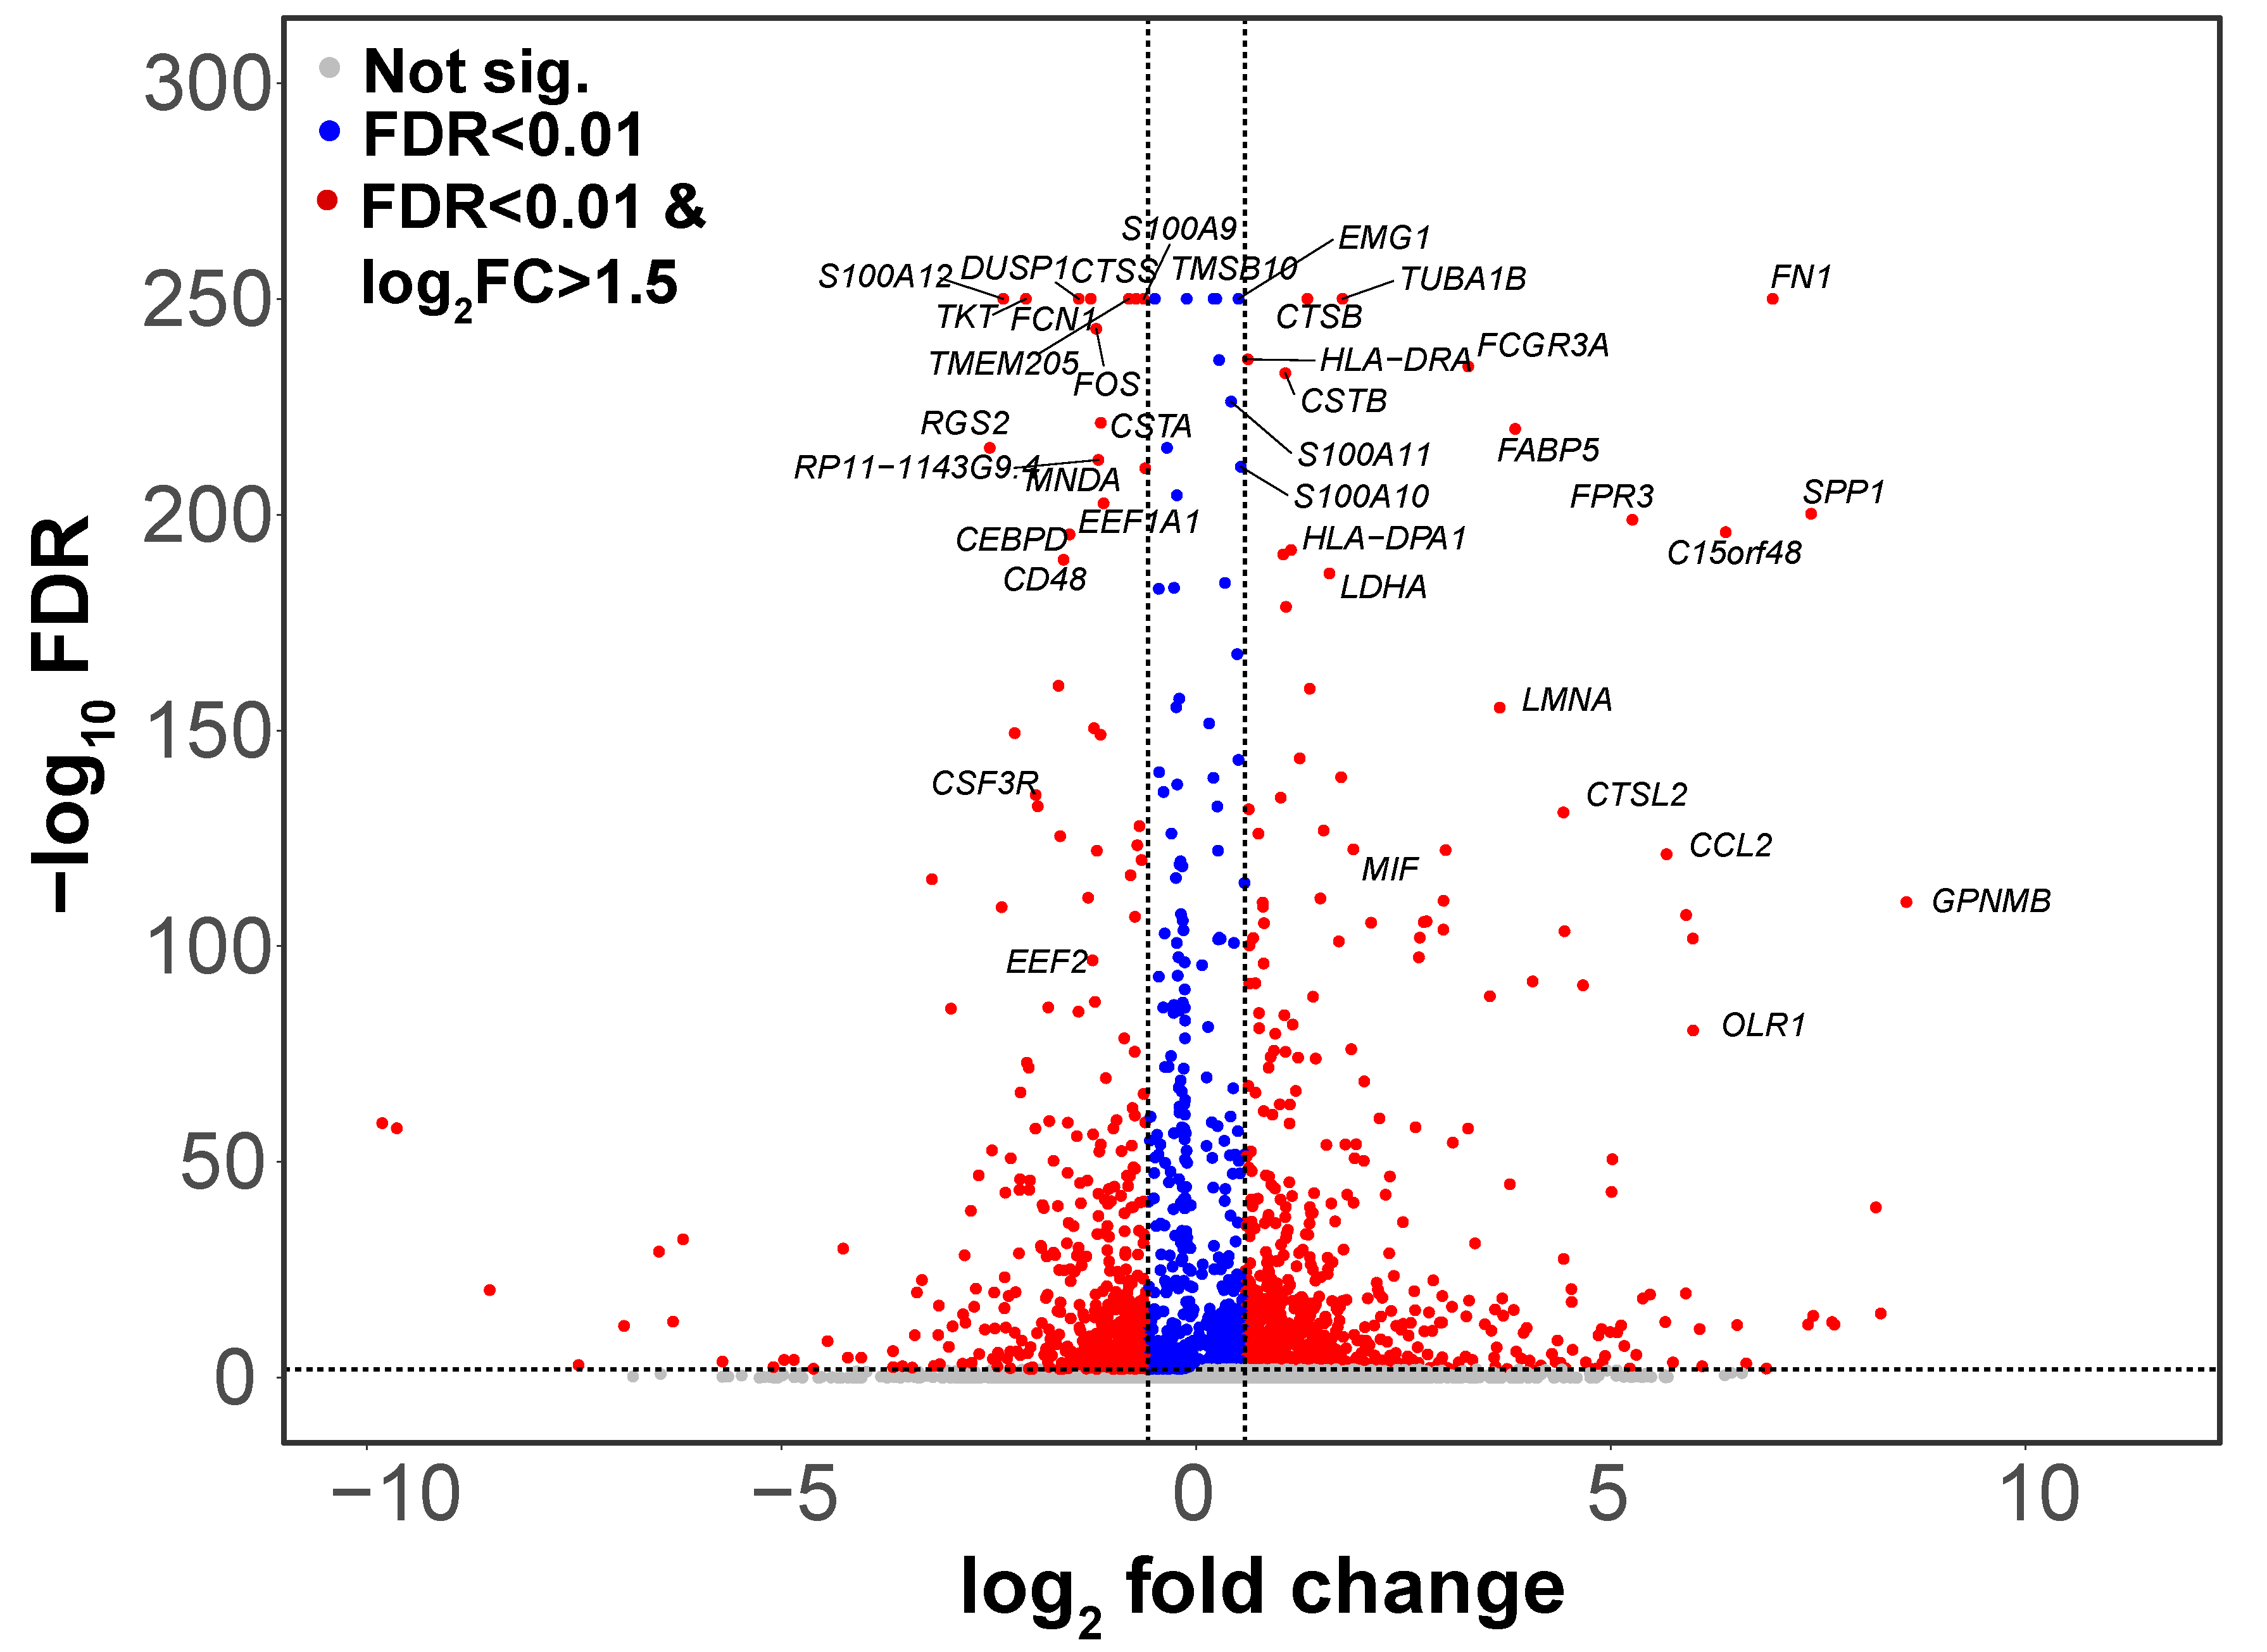
\includegraphics[width=0.7\textwidth]{./Results3/pdfs/PSA_monocytes_scanpy_single_cell_SFvsPB_volcano_plot_differential_analysis_less_labels}
%\caption[Contrast between synovial fluid and peripheral blood CD14$^+$ monocytes using sc-RNA-seq and correlation with ATAC differential accessible regions.]{\textbf{Contrast between synovial fluid and peripheral blood CD14$^+$ monocytes using sc-RNA-seq and correlation with ATAC differential accessible regions.} Volcano plots showing differences in gene expression between synovial fluid and peripheral blood CD14$^+$ monocyte using scRNA-seq data. The significance (log$_{10}$FDR) of the differential expression (y-axis) is plotted against the log${_2}$fold change, where a positive fold change indicates higher expression in CD14$^+$ monocytes from synovial fluid compared to peripheral blood and viceversa. Genes are coloured based on FDR and log$_{2}$fold changes and some of the top significant genes are labelled.}
%\label{figure:PSA_monocytes_scanpy_single_cell_volcano_plots_and_ATAC_correlation}
%\end{figure}



%\begin{figure}[htbp]
%\centering
%\includegraphics[width=0.6\textwidth]{./Appendix/pdfs/Chapter5/PsA_FM_SNPs_overlap_eQTL_one_SNP_per_eGene}
%\caption[Enrichment of PsA GWAS fine-mapped SNPs for publicly available eQTL datasets.]{\textbf{Enrichment of PsA GWAS fine-mapped SNPs for publicly available eQTL datasets.} The percentage of SNPs from the combined 90\% credible setx SNPs of the seven successfully fine-mapped PsA loci overlapping SNPs from publicly available eQTL datasets (immune cell types and GTeX) are shown (red dot). This overlap is compared to the distribution of overlaps with the same eQTL datasets for each of the 1,000 sets of background SNPs (boxplots). Significance of the enrichment is indicated as p-value calculated using binomial test.}
%\label{figure:PSA_fine_mapping_eQTL_enrichment}
%\end{figure}


%\begin{figure}[htbp]
%\centering
%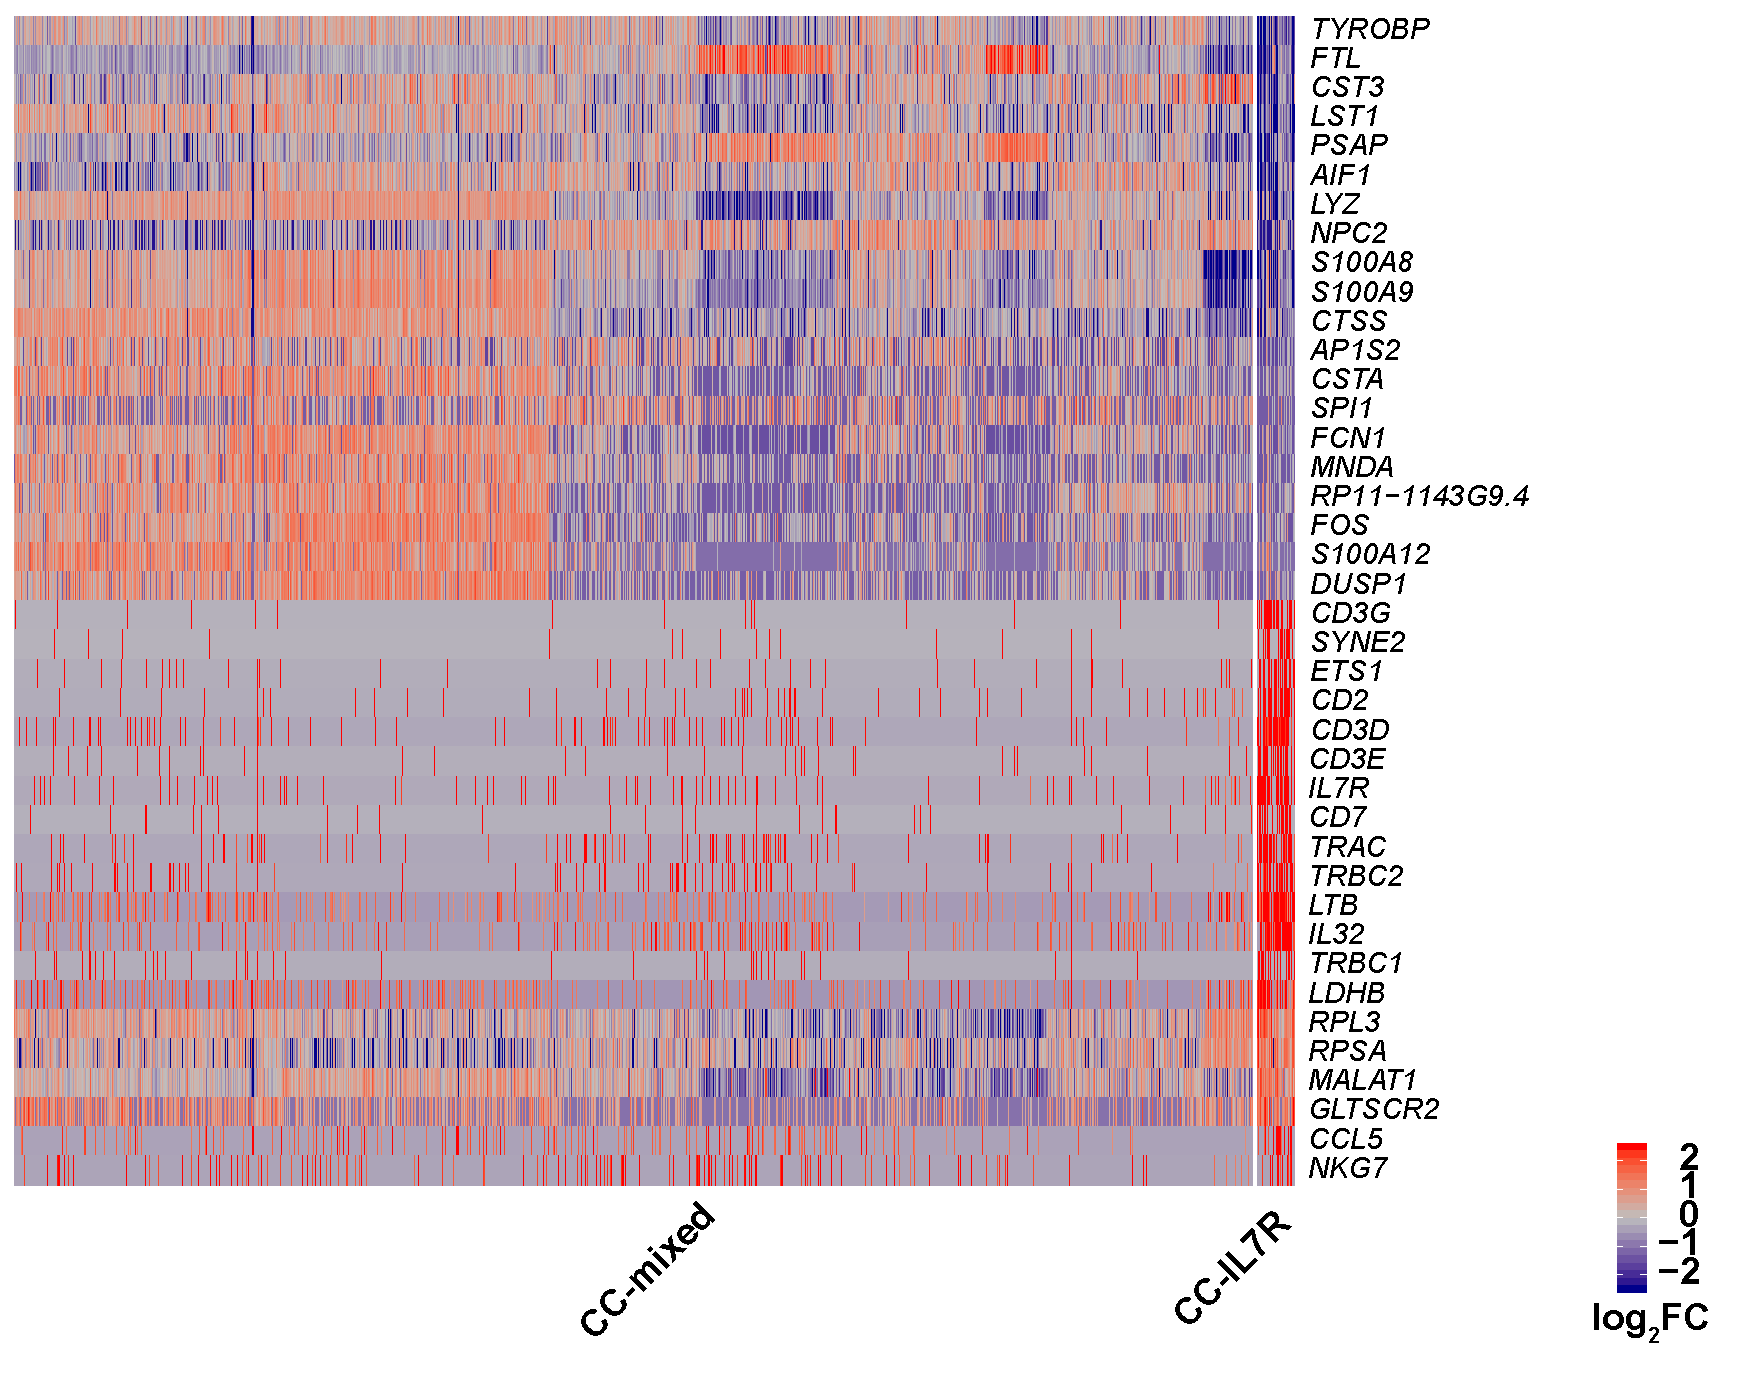
\includegraphics[width=0.6\textwidth]{./Appendix/pdfs/Chapter5/PSA_10X_heatmap_SF_PB_monocytes_clusters_mixed_and_IL7R}
%\caption[Heatmap for the top 20 marker genes of the CC-mixed and CC-IL32 CD14$^+$ monocytes subpopulations.]{\textbf{Heatmap for the top 20 marker genes of the CC-mixed and CC-IL32 CD14$^+$ monocytes subpopulations.} Rows are the top 20 marker genes for each of the two subpopulations (total of 40 genes). The columns represent each of the cells members of the CC-mixed (left) or CC-IL32 (right) clusters. The colour scale represents the log$_2$FC in the expression of the marker gene in a particular cell of the cluster compared to the average expression of all the cells from the other cluster.}
%\label{figure:PSA_scRNAseq_CC_mixed_and_IL32_markers_heatmap}
%\end{figure}
%

%
%\begin{figure}[htbp]
%\centering
%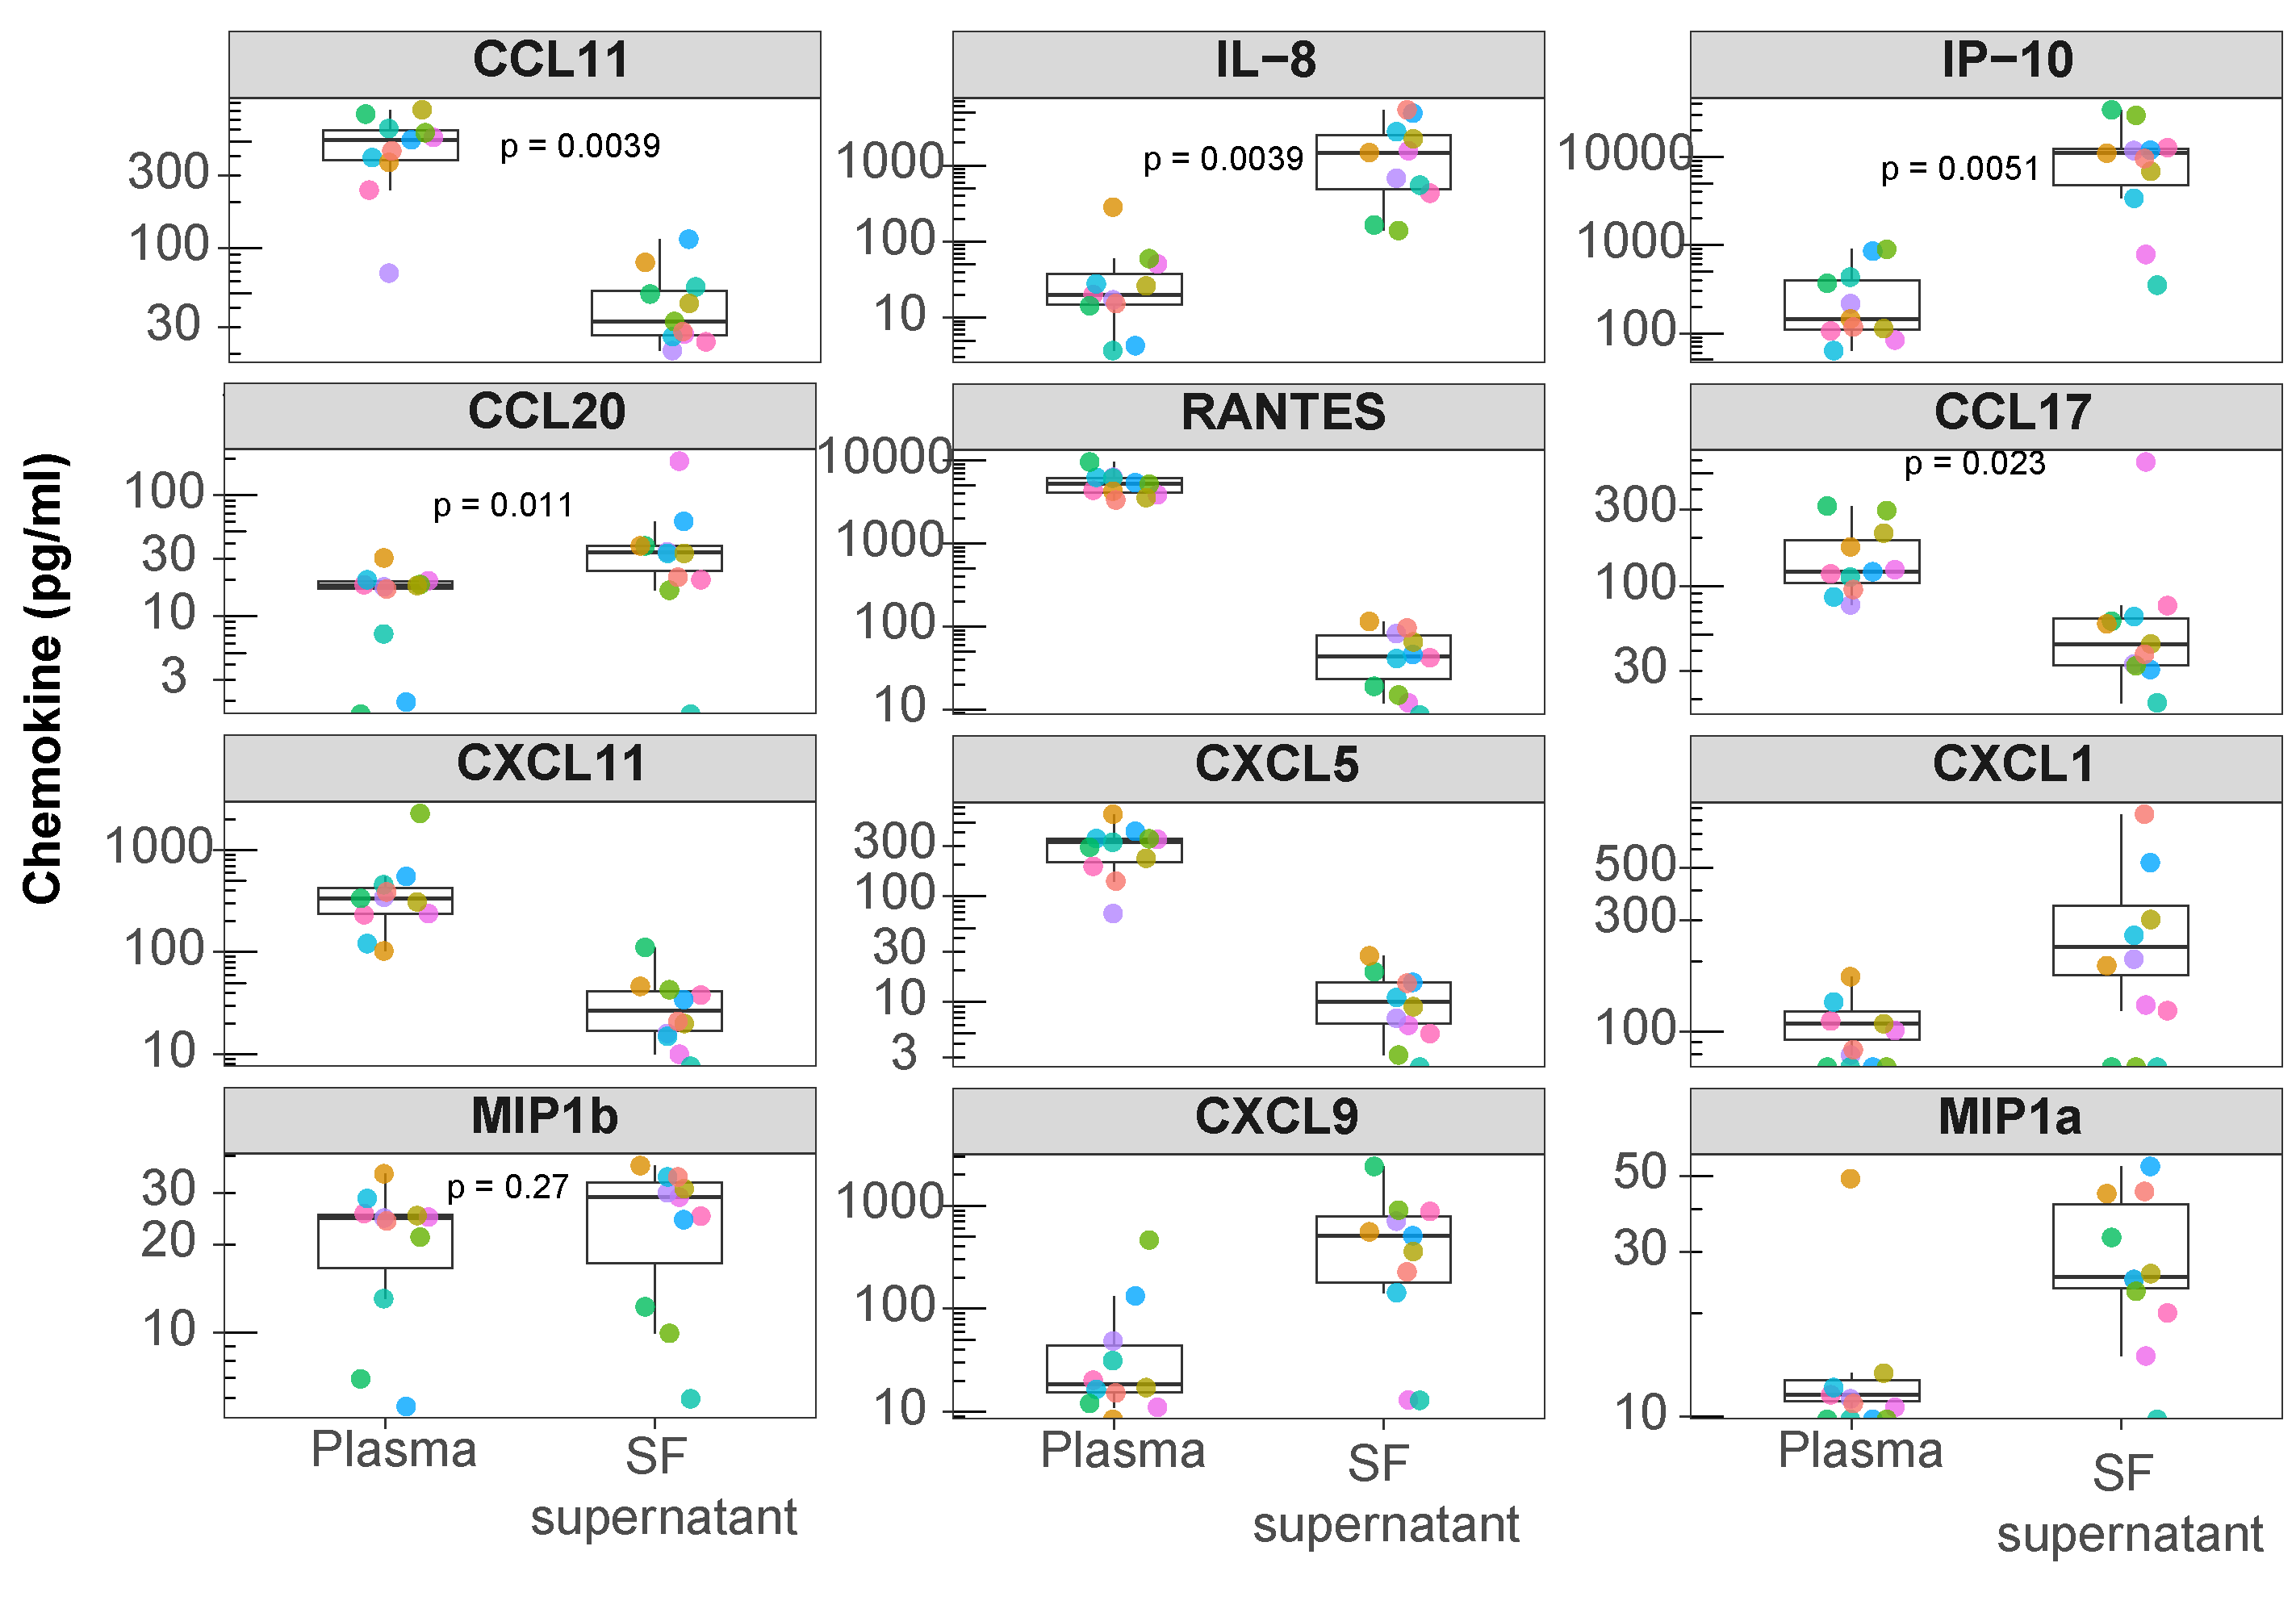
\includegraphics[width=1.0\textwidth]{./Appendix/pdfs/Chapter5/ELISA_plasma_synovial_fluid_10_samples}
%\caption[Quantification of cytokine levels in plasma and synovial fluid from 10 PsA patients.]{\textbf{Quantification of cytokine levels in plasma and synovial fluid from 10 PsA patients.} Boxplots illustrating the concentration in pg/mL (x-axis log$_{10}$ scale) for a number of cytokines measured in supernatant from synovial fluid and plasma from peripheral blood of 10 PsA patients. The experiment was conducted by collaborators in Basle using enzyme-linked immunosorbent assay (ELISA). Each circle represents one sample and patient identity is colour coded. For some of the cytokines, the significance of the difference in concentration between the two tissues has been determined using Wilcoxon signed-rank test and the corresponding p-value is included.}
%\label{figure:ELISA_SF_PsA}
%\end{figure}
